\documentclass[a4paper,UKenglish,cleveref,pdftex,thm-restate,numberwithinsect]{lipics-v2021}
\usepackage{stmaryrd}
\usepackage{bbding}
%\Envelope
\newcommand{\cat}[1]{\ensuremath{\mathbf{#1}}}

\newcommand{\pbc}{\mathsf{Pb}}
\usepackage{amsthm,amsmath,amssymb,mathrsfs, dsfont}
\usepackage{tikz-cd}
\usepackage{hyperref, cleveref} %simboli matematici
\usepackage[all, cmtip]{xy}

\usepackage[utf8]{inputenc} % Input encoding - per caratteri particolari
%\usepackage[english]{babel} % Lingua principale inglese
\usepackage{graphicx} % Per includere immagini esterne
\usepackage[tickmarkheight=.5em,textwidth=\marginparwidth,textsize=small]{todonotes}
\usepackage{mathtools}
\usepackage{csquotes}


\usepackage{tikz-cd}

%String Diagrams
\usepackage{tikz}
\usepackage[draft]{tikzit}
\input{hypergraph.tikzdefs}
\input{hypergraph.tikzstyles}


\usetikzlibrary{decorations.markings}

% General Setting diagrams
%\usepackage{tikz-cd} %diagrammi
%\tikzcdset{row sep/normal=5em}
%\tikzcdset{column sep/normal=5em}
%\tikzcdset{every label/.append style = {font = \small}}

%\spnewtheorem*{notation}{Notation}{\bfseries}{}
%\spnewtheorem*{convention}{Convention}{\bfseries}{}



%funtori
\usepackage[usestackEOL]{stackengine}
\newcommand\functorop[1][l]{\csname#1functor\endcsname}
\newcommand\lfunctorop[3]{%
	\setbox0=\hbox{$#2$}%
	\kern\wd0%
	\ensurestackMath{\Centerstack[c]{#1\\ \mathllap{#2\;\,}\mathclap{\DownArrow}\\#3}}%
}		
\newcommand\rfunctorop[3]{%
	\setbox0=\hbox{$#2$}%
	\ensurestackMath{\Centerstack[c]{#1\\\mathclap{\UpArrow}\mathrlap{\,\;#2}\\#3}}%
	\kern\wd0%
}
\newcommand\functoropmapsto{\mathrel{\ensurestackMath{\Centerstack[c]{\longmapsto\\ \\\longmapsto}}}}
\setstackgap{L}{1.3\normalbaselineskip}
\newcommand\UpArrow{\rotatebox[origin=c]{90}{$\longrightarrow$\,}}
\newcommand\DownArrow{\rotatebox[origin=c]{-90}{$\longrightarrow$\,}}
\newcommand\functor[1][l]{\csname#1functor\endcsname}
\newcommand\lfunctor[3]{%
	\setbox0=\hbox{$#2$}%
	\kern\wd0%
	\ensurestackMath{\Centerstack[c]{#1\\ \mathllap{#2\;\,}\mathclap{\DownArrow}\\#3}}%
}
\newcommand\rfunctor[3]{%
	\setbox0=\hbox{$#2$}%
	\ensurestackMath{\Centerstack[c]{#1\\\mathclap{\DownArrow}\mathrlap{\,\;#2}\\#3}}%
	\kern\wd0%
}
\newcommand\functormapsto{\mathrel{\ensurestackMath{\Centerstack[c]{\longmapsto\\ \\\longmapsto}}}}
\setstackgap{L}{1.3\normalbaselineskip}

\newcommand{\lgh}{\mathsf{lg}}
\newcommand{\eq}{\mathsf{eq}}
\newcommand{\quo}{\mathsf{Q}}

\DeclareMathAlphabet{\mymathbb}{U}{BOONDOX-ds}{m}{n}

\newcommand{\Ob}{\mathcal{O}b}
\newcommand{\Hom}{\mathcal{H}om}
\newcommand{\Set}{\mathbf{Set}}
\newcommand{\Reg}{\mathcal{Reg}}
\newcommand{\Mono}{\mathcal{Mono}}
\newcommand{\initial}{\mymathbb{0}}
\newcommand{\terminal}{\mathds{1}}
\newcommand{\eg}[1]{\mathbf{EqGraph}_{\textbf {\textup{#1}}}}
%\newcommand{\egg}[1]{\mathbf{EGG}_{\textbf {\textup{#1}}}}

\makeatletter
\def\@citecolor{blue}%
\def\@urlcolor{blue}%
\def\@linkcolor{blue}%
\def\UrlFont{\rmfamily}
\def\orcidID#1{\smash{\href{http://orcid.org/#1}{\protect\raisebox{-1.25pt}{\protect
\includegraphics{orcid_color.eps}}}}}
\makeatother



\def\R{\mathsf{R}}
\def\B{\textbf {\textup{B}}}
\def\C{\textbf {\textup{C}}}
\def\D{\textbf {\textup{D}}}
\def\X{\textbf {\textup{X}}}
\def\Y{\textbf {\textup{Y}}}
\def\E{\textbf {\textup{E}}}
\def\T{\textbf {\textup{1}}}
\def\A{\textbf {\textup{A}}}
\def\M{\mathcal{M}}
%categorie varie
\newcommand{\catname}[1]{\textbf{\textup{#1}}}
\newcommand{\lab}{\catname{LHyp}}
\newcommand{\hyp}{\catname{Hyp}}
\newcommand{\hyps}{\catname{Hyp}_{\Sigma}}
\newcommand{\EqHyp}{\catname{EqHyp}} %equivalence hypergraphs
\newcommand{\EqHyps}{\catname{EqHyp}_{\Sigma}}
\newcommand{\EqTG}{\catname{EqTG}}
\newcommand{\EqTGs}{\catname{EqTG}_{\Sigma}}
\newcommand{\GEqTGs}{\catname{GEqTG}_{\Sigma}}
\newcommand{\GEqATGs}{\catname{GEqATG}_{\Sigma}}
\newcommand{\gr}{\textbf{\textup{Graph}}}
\newcommand{\dgr}{\catname{SGraph}}
\newcommand{\dg}{\catname{DAG}}
\newcommand{\rt}{\mathsf{dcl_s}}
\newcommand{\rta}{\mathsf{dcl}}
\newcommand{\rtd}{\mathsf{dcl_{d}}}
\newcommand{\slice}[2]{(\catname{#1}\downarrow{#2})}
\newcommand{\tg}[0]{\catname{TG}_{\Sigma}}
\newcommand{\teg}[0]{\catname{TeGr}_{\Sigma}}
\newcommand{\sv}[0]{\mathsf{Sieves}}
\newcommand{\mono}[1]{\mathsf{Mon}(\catname{#1})}
\newcommand{\mo}[1]{{#1}_\mathsf{Mon}}
\newcommand{\pro}{\mathsf{prod}}
\newcommand{\spro}{\mathsf{ps}}
\newcommand{\prol}{\mathsf{lprod}}
\newcommand{\pred}[1]{{\downarrow}#1}
\newcommand{\colim}[0]{\mathrm{colim}}
\newcommand{\cod}{\mathsf{cod}}
\renewcommand{\sp}{\mathsf{sp}}
\renewcommand{\sup}{\mathsf{sup}}
\newcommand{\cow}[1]{\mathsf{cwd}({#1})}
\renewcommand{\inf}{\mathsf{inf}}
\newcommand{\dom}{\mathsf{dom}}
\newcommand{\dwnarrow}{\downarrow \hspace{-2pt}}
\newcommand{\Dwnarrow}{\Downarrow \hspace{-2pt}}
\newcommand{\egg}{\catname{GEqHyp}}

\newcommand{\ari}{\mathsf{ar}}
\newcommand{\abs}[1]{\lvert #1\rvert}


\newcommand{\upstr}[1] { {#1}^{\uparrow }}
\newcommand{\comma}[2]{#1\hspace{1pt} {\downarrow}#2}
\newcommand{\cma}[2]{\mathcal{#1}\hspace{1pt} {\downarrow}\hspace{1pt} \mathcal{#2}}

\newcommand{\commentato}[1]{ {} }

%sommatoria e prodotto per xy

\usepackage{relsize}
\newcommand{\Sum}{\mathlarger{\sum}}
\newcommand{\Prod}{\mathlarger{\prod}}

\bibliographystyle{abbrv}

%frecce
\newcommand{\mor}{\mathsf{Mor}}
\newcommand{\mon}{\mathsf{Mono}}
\newcommand{\reg}{\mathsf{Reg}}
\newcommand{\mto}{\rightarrowtail}
\newcommand{\eto}{\twoheadrightarrow}
\newcommand{\id}[1]{\mathsf{id}_{#1}}

\tikzset{->-/.style={decoration={
			markings,
			mark=at position #1 with {\arrow{>}}},
			postaction={decorate}
			}}

\title{EGGs are adhesive!}
\titlerunning{EGGs are adhesive!} %TODO optional, please use if title is longer than one line

% Author with single affiliation.
\author{Roberto Biondo}
{Department of Computer Science, University of Pisa, Pisa, IT}
{r.biondo@studenti.unipi.it}{}{}

\author{Davide Castelnovo}
{Department of Computer Science, University of Pisa, Pisa, IT}
{castelnovod@gmail.com}
{https://orcid.org/0000-0002-5926-5615}{}

\author{Fabio Gadducci}
{Department of Computer Science, University of Pisa, Pisa, IT}
{fabio.gadducci@unipi.it}
{https://orcid.org/0000-0003-0690-3051}{}

\authorrunning{R.~Biondo, D.~Castelnovo, F.~Gadducci}

\Copyright{Roberto Biondo and Davide Castelnovo and Fabio Gadducci} 
\ccsdesc[500]{Theory of Computation~Models of computation}
\ccsdesc[500]{Theory of Computation~Semantics and reasoning}

\keywords{Hypergraphs, terms graphs, e-graphs, adhesive categories.} %TODO mandatory; please add comma-separated list of keywords

\funding{The research has been partially supported by the Italian MUR - Call PRIN 2022 - Project 20228KXFN2 ``Spatio-Temporal Enhancement of Neural nets for Deeply
Hierarchical Automatised Logic'' (STENDHAL) 
and by the University of Pisa - Call PRA 2022 - Project 2022\_99 ``Formal Methods for the Healthcare Domain based on Spatial Information'' (FM4HD).}

\begin{document}

\maketitle

\begin{abstract}
The use of rewriting-based visual formalisms is on the rise. 
%
In the formal methods community, this is due also to the introduction of adhesive
categories, where most properties of classical approaches to graph transformation, 
such as those on parallelism and confluence, can be rephrased and proved in a general and 
uniform way.
%
E-graphs (EGGs) are a formalism for program optimisation 
via an efficient implementation of equality saturation. 
In short, EGGs can be  defined as (acyclic) term graphs with an additional notion of 
equivalence on nodes that is closed under the operators of the signature.
Instead of replacing the components of a program, the optimisation step 
is performed by adding new components and linking them to 
the existing ones via an equivalence relation, until an optimal program is reached.
%
This work describes EGGs via adhesive categories. 
Besides the benefits in itself of a formal presentation, which renders the 
properties of the data structure precise, the description of the addition of equivalent 
program components using standard graph transformation tools offers the advantages 
of the adhesive framework in modelling, for example, concurrent updates.
%
%Besides 
%the benefits \emph{per se} of a formal presentation, making precise the properties of 
%the data structure, describing the addition of equivalent program components 
%via the standard tools of graph transformation offers the advantages given by the 
%adhesive framework in modelling e.g. concurrent updates.
\end{abstract}


\section{Introduction}
The introduction of \emph{adhesive categories} marked a watershed moment for the algebraic approaches 
to the rewriting of graph-like structures~\cite{lack2005adhesive,ehrig2006fundamentals}.
%
Until then, key results of the approaches on e.g. parallelism and confluence had to be proven 
over and over again for each different formalism at hand, %let it be either xxx or xx, 
despite the obvious similarity of the procedure.
%
Adhesive categories provides such a disparate set of formalisms with a common abstract framework 
where many of these general results could be recast and uniformly proved once and for all.
 
\vspace{.1cm}
\noindent
\begin{minipage}[l]{.78\linewidth}In short, following the double-pushout (DPO) approach
to graph transformation~\cite{xxx}, a rule is given by two arrows $l: K \to L$ and $r: K \rightarrow R$
and its execution requires a match $m: L \to G$ such that the rewriting step from $G$
to $H$ is given by the diagram aside, whose square are pushouts.
  \end{minipage}%
    \hfill
  \begin{minipage}[r]{.20\linewidth }
    \xymatrix@C=.5cm@R=.5cm{
      L \ar[d]_{m}
      & K \ar[r]^r \ar[l]_{l} \ar[d] & R \ar [d] \\
      G & C \ar[r] \ar[l]                    & H
    }
%    \xymatrix@C=.5cm@R=.5cm{
%      L \ar[d]_{m} \ar@{}[dr]|{(1)}
%      & I \ar[r]^r \ar@{>->}[l]_{l} \ar[d] \ar@{}[dr]|{(2)} & R \ar [d] \\
%      G & C \ar@{->}[r] \ar@{>->}[l]                    & H\\
 %     & J \ar@{->}[ul] \ar@{->}[u]|{k} \ar@{->}[ur]
 %   }
  \end{minipage}
\vspace{.1cm}

\noindent
Thus, $L$ and $R$ are the lift- and right-hand side of the rule, respectively, while $K$ witnesses those parts that must 
be present for the rule to be executed, yet they are not affected by the rule itself.
%
If a category is adhesive, and the arrows of the rules are monomorphisms, then the presence of a match ensures that the
two pushouts exist, hence a rewriting step can be performed.
%
The theory of $\mathcal{M}$-adhesivity~\cite{xxx} extend the core framework, still ensuring that if the arrow 
of the rules are in $\mathcal{M}$,
%and the match is in $\mathcal{N}$, 
then the classical results from the theory of graph 
transformation can still be lifted~\cite{xxx}. 
If only the left-hand side belongs to $\mathcal{M}$, the current theory is stil under development, as witnessed e.g.
by~\cite{BaldanC0G24}.
%
However, despite the elegance and effectiveness and the immediate advantages of proving a category 
to be adhesive, proving that a given category satisfies the conditions 
for being adhesive can be a daunting task. For this reason,  sufficient criteria have been provided for the core 
framework, e.g. that every elementary topos is adhesive \cite{lack2006toposes}, as well as for the extended one of
$\mathcal{M}$-adhesivity~\cite{CastelnovoGM24}.
%
For some graph-like structures, such as those called \emph{hypergraph with equivalence} in~\cite{concur2006}, the question 
of their adhesivity has not yet been settled.

\emph{E-graphs} (shortly, EGGs) are an up-and-coming formalism for program optimisation and synthesis via a compact 
representation and efficient implementation of equality saturation. 
%
Albeit a classical data structure~\cite{DetlefsNS05}, EGGs received 
new impulse after the seminal~\cite{WillseyNWFTP21} and
developed a thriving community, as witnessed by the official website~\cite{eggs}.
%
The key idea of rewriting-based program optimisation is to perform the manipulation of a syntactical description 
of a program, replacing some of its components in such a way that the semantics is preserved while 
the computational costs of its actual execution are improved. Instead of directly removing sub-programs, EGGs just add the 
new components and link them to the older ones via the equivalence relation, until an optimal program is 
reached and extracted.

EGGs can be concisely defined as (acyclic) term graphs with an additional notion of equivalence on nodes
that is closed under the operators of the signature~\cite[Section~4.2]{DetlefsNS05}.
In the presentation of term graphs via string diagrams~\cite{CastelnovoGM24}, EGGs are (hyper)trees equipped with 
the possibility of sharing subtrees, as in terms graphs, with an additional equivalence relation $\equiv$ on nodes that 
is closed under composition. In plain words and using a toy example:
if $a$ and $b$ are two constants such that $a \equiv b$, then $f(a) \equiv f(b)$ for any unary operator $f$.


%EGGs received a lot of attention in the implementation  side, as it is natural, since they have been introduced precisely as
%a fast way to recover equality saturation. 

Building on the criterion developed in~\cite{CastelnovoGM24}, this work proves that both hypergraphs with equivalence
and EGGs form an 
$\mathcal{M}$-adhesive category for a suitable choice of $\mathcal{M}$.
The advantages from this characterisation are two-fold. On the one side, 
we put the benefits \emph{per se} of a formal presentation, making precise the properties of the data structure. 
On the other side, describing the optimisation steps via the DPO approach
offers the tools for modelling their parallel and concurrent execution
and for proving their confluence and termination.

\emph{Synopsis}
The paper has the following structure. 
In Section~\ref{sec:ade} we briefly recall 
the theory of $\mathcal{M}$-adhesive categories
and of kernel pairs.
In Section~\ref{sec:hyper} we present the graphical structures of our interest, 
 (labelled) hypergraphs and term graphs, and we provide a
functorial characterisation, which allows for proving their adhesivity properties.
This is expanded in Section~\ref{hypereq} for proving the $\mathcal{M}$-adhesivity
of hypergraphs 
and term graphs with equivalence and in Section~\ref{eggs} of
their variants where equivalences are closed with respect to operator application,
thus subsuming EGGs.
%
In Section~\ref{rewriting} we put the machinery at work, showing how the optimisation steps
can be rephrased as the application of term graph rewriting rules.
%
Finally, in Section~\ref{conclusioni} we draw our conclusions, hint at future endeavours and offer some 
brief remarks on related works.
%
For the sake of space, the proofs appear in the appendices. 
%For the sake of completeness, 
%and in order to fix the notation, we prove all the results 
%recalled in the background section, besides those that are original 
%to our work.

\section{Facts about $\mathcal{M}$-adhesive categories and kernel pairs}\label{sec:ade}


%
%\begin{notation}
We open this background section by fixing some notation.
%
Given a category $\X$ we do not distinguish notationally between $\X$ and its class of objects, so
``$X\in \X$'' means that $X$ is an object of $\X$. We let $\mor(\X)$, $\mon(\X)$ and $\reg(\X)$ denote the class of all arrows, monos and regular monos of $\X$, respectively.  Given an object $X$, we  denote by $?_X$ the unique arrow from an initial object into $X$ and by $!_X$ that  unique arrow from $X$ into a terminal one. We will also use the notation $e\colon X\eto Y$ to denote that an arrow $e\colon X\to Y$ is a regular epi. 
%\end{notation}

\subsection{$\mathcal{M}$-adhesivity}\label{subsec:ade}
The key property of $\mathcal{M}$-adhesive categories is the \emph{Van Kampen condition}~\cite{brown1997van,johnstone2007quasitoposes,lack2005adhesive},
%
and for defining it we need some notions.
%and to define it we introduce some notions.  
Let  $\X$ be a category. A subclass $\mathcal{A}$ of $\mor(\X)$ is said to be

\parbox{11cm}{\begin{itemize}
	\item		\emph{stable under pushouts (pullbacks)} if for every pushout (pullback) square as the one aside, if $m \in \mathcal{A}$ ($n\in \mathcal{A}$) then $n \in \mathcal{A}$ ($m \in \mathcal{A}$);
		\item \emph{closed under composition} if $h, k\in \mathcal{A}$ implies $h\circ k\in \mathcal{A}$ whenever $h$ and $k$ are composable.
\end{itemize}}\hfill
\parbox{1cm}{
\xymatrix{A \ar[r]^{f} \ar[d]_{m}& B \ar[d]^{n} \\ C \ar[r]_{g} & D}}

	\begin{definition}
	
	Let $\mathcal{A}\subseteq \mor(\X)$ be a class of arrows in a category $\X$ and consider the cube below on the right. 

\vspace{-.25cm}
\parbox{9.5cm}{We say that the bottom square is an \emph{$\mathcal{A}$-Van Kampen square} if
	\begin{enumerate}
		\item it is a pushout square;
		\item 	whenever the cube above has pullbacks as back and left faces and the vertical arrows belong to $\mathcal{A}$, then its top face is a pushout 
		if and only if the front and right faces are pullbacks.
	\end{enumerate}} \hfill
	\parbox{3cm}{
	\xymatrix@C=10pt@R=6pt{&A'\ar[dd]|\hole_(.65){a}\ar[rr]^{f'} \ar[dl]_{m'} && B' \ar[dd]^{b} \ar[dl]_{n'} \\ C'  \ar[dd]_{c}\ar[rr]^(.7){g'} & & D' \ar[dd]_(.3){d}\\&A\ar[rr]|\hole^(.65){f} \ar[dl]^{m} && B \ar[dl]^{n} \\C \ar[rr]_{g} & & D }
}


	Pushout squares that enjoy only the ``if'' half of item (2) above are called \emph{$\mathcal{A}$-stable}. A $\mor(\X)$-Van Kampen square is called  \emph{Van
		Kampen} and a $\mor(\X)$-stable square  \emph{stable}.
\end{definition}

We can now define $\mathcal{M}$-adhesive categories.

\begin{definition}[\cite{azzi2019essence,ehrig2012,ehrig2014adhesive,lack2005adhesive,heindel2009category}]
	Let $\X$ be a category and $\mathcal{M}$ a subclass of
	$\mon(\X)$  including  all isos, closed under composition,  and stable under pullbacks and pushouts.  The category  $\X$ is said to be \emph{$\mathcal{M}$-adhesive} if
	\begin{enumerate}
		\item it has \emph{$\mathcal{M}$-pullbacks}, i.e.~pullbacks along arrows of $\mathcal{M}$;
		\item it has \emph{$\mathcal{M}$-pushouts}, i.e.~pushouts along arrows of $\mathcal{M}$;
		\item  $\mathcal{M}$-pushouts are $\mathcal{M}$-Van Kampen squares.
	\end{enumerate}
	%
	A category $\X$ is said to be \emph{strictly $\mathcal{M}$-adhesive}
	if $\mathcal{M}$-pushouts are Van Kampen. We write $m\colon X \mto Y$ to denote that an arrow $m\colon X\to Y$ belongs to $\mathcal{M}$.
\end{definition}



\begin{remark}
	\label{rem:salva}
	\emph{Adhesivity} and \emph{quasiadhesivity} 
	\cite{lack2005adhesive,garner2012axioms} coincide with strict
	$\mon(\X) $-adhesivity and strict $\reg(\X)$-adhesivity,
	respectively.
\end{remark}


$\mathcal{M}$-adhesivity is well-behaved with respect to  the construction of slice and functor categories \cite{mac2013categories}, as shown by the following theorems~\cite{ehrig2006fundamentals,lack2005adhesive}.

\begin{proposition}
	\label{thm:slice-functors}
	Let $\X$ be an (strict) $\mathcal{M}$-adhesive category. Then it holds
	\begin{enumerate}
		\item if $\Y$ is an (strict) $\mathcal{N}$-adhesive category $L\colon \Y\to \A$ a functor preserving $\mathcal{N}$-pushouts and $R\colon \X\to A$ one preserving pullbacks, then $\comma{L}{R}$ is (strictly) $\comma{\mathcal{N}}{\mathcal{M}}$-adhesive, where
		\[\comma{\mathcal{N}}{\mathcal{M}}:=\{(h,k) \in \mor(\comma{L}{R}) \mid h\in \mathcal{N}, k\in \mathcal{M}\}\]
		\item for every object $X$
		the categories $\X/X$  and $X/X$ are, respectively, (strictly) $\mathcal{M}/X$-adhesive and (strictly) $X/\mathcal{M}$-adhesive, where
		\[\mathcal{M}/X:=\{m\in \mor(\X/X) \mid m\in
		\mathcal{M}\} \hspace{5pt} X/\mathcal{M}:=\{m\in \mor(X/\X) \mid m\in \mathcal{M}\}\]
		\item for every small category $\Y$, the category $\X^\Y$ of
		functors $\Y\to \X$ is (strictly) $\mathcal{M}^{\Y}$-adhesive, where
		$\mathcal{M}^{\Y}:=\{\eta \in \mor(\X^\Y) \mid \eta_Y \in
		\mathcal{M} \text{ for every } Y\in \Y\}$;
		\item if $\Y$ is a full subcategory of $\X$ closed in it under pullbacks and $\mathcal{M}$-pushouts, then $\Y$ is (strictly) $\mathcal{N}$-adhesive for every class of arrows $\mathcal{N}$ of $\Y$ contained in $\mathcal{M}$ that is stable under pullbacks and pushouts, contains all isos, and is closed under composition and decomposition.
	\end{enumerate} 
\end{proposition}

We briefly list some examples of $\mathcal{M}$-adhesive categories.

\begin{example}
	\label{ex:adhesive}
	$\cat{Set}$ is adhesive, and, more generally, every topos is
	adhesive~\cite{lack2006toposes}. By the closure properties above, every presheaf $[\cat{X},\cat{Set}]$ is adhesive, thus the category
	$\cat{Graph} = [ E \rightrightarrows V, \cat{Set}]$ is adhesive
	where $E \rightrightarrows {V}$ is the two objects category with two
	morphisms $s,t \colon{E} \to {V}$. Similarly, various
	categories of hypergraphs can be shown to be adhesive, such as term
	graphs and hierarchical graphs~\cite{CastelnovoGM24}. Note that the category $\cat{sGraphs}$ of simple graphs, 
	i.e.~graphs without parallel edges, is
	$\reg{(\cat{sGraphs})}$-adhesive~\cite{BehrHK23} but not
	quasiadhesive.
\end{example}

\iffalse 
\begin{remark}\label{rem:deco}
We can point out an important property of strict $\mathcal{M}$-adhesive categories with pullbacks.  Consider the solid part of the cube aside, whose bottom case is an $\mathcal{M}$-pushout.
	
	\parbox{9.5cm}{	Given an arrow $d\colon X\to D$, we can present the object $X$ has a pushout: indeed, consider the following cube, in which all the three vertical squares are pullbacks.}
	\parbox{3cm}{
	\xymatrix@C=15pt@R=9pt{&V\ar[dd]|\hole_(.65){a}\ar[rr]^{v} \ar@{>.>}[dl]_{u} && Y \ar[dd]^{b} \ar@{>->}[dl]_{y} \\ Z  \ar[dd]_{c}\ar[rr]^(.7){z} & & X \ar[dd]_(.3){d}\\&A\ar[rr]|\hole^(.65){f} \ar@{>->}[dl]^{m} && B \ar@{>->}[dl]^{n} \\C \ar[rr]_{g} & & D }}

Now, notice that, since the front square is a pullback, then the dotted arrow $u\colon V\to Z$ exists. Moreover, the usual composition and decomposition property of pullbacks \cite{mac2013categories} entails that the left face of the cube so obtained is a pullback too, proving that $u$ is in $\mathcal{M}$ and that the top square is a pushout.

	Clearly if the arrow $p\colon X\to D$ is in $\mathcal{M}$, we can omit the assumptions of strictness and the existence of all pullbacks.
\end{remark}
\fi 


We can state some useful properties of $\mathcal{M}$-adhesive category.

\begin{restatable}{proposition}{regmono}\label{prop:regmono}
	Let $\X$ be an $\mathcal{M}$-adhesive category. Then it holds
	\begin{enumerate}
		\item every $\mathcal{M}$-pushout square is also a pullback;
		\item every arrow in $\mathcal{M}$ is a regular mono.
	\end{enumerate}
\end{restatable}
%  [Proof in \Cref{regmono-proof}]


\subsection{Some properties of kernel pairs and regular epimorphisms}

In this section we recall the definition and some properties of \emph{kernel pairs}.
%which will be useful in the next sections. 

\noindent 
\parbox{11cm}{
\begin{definition}
    A \emph{kernel pair} for an arrow $f\colon A \to B$ is an object $K_f$ together with two arrows $\pi^1_f, \pi^2_f\colon K_f \rightrightarrows A$, denoted as $(K_f, \pi^1_f, \pi^2_f)$, such that the square aside is a pullback.
\end{definition}}\hfill 
\parbox{2cm}{\xymatrix@R=15pt{K_f \ar[r]_{\pi^2_f} \ar[d]_{\pi^1_f}& A \ar[d]^f \\ A \ar[r]^{f}& B}}

\smallskip
\begin{remark}\label{prop:pairng_of_kernel_pairs_mono}
If $(K_f, \pi^1_f, \pi^2_f)$ is a a kernel pair for $f\colon X \to Y$ and a product of $X$ with itself exists, then the canonical arrow $\langle \pi^1_f, \pi^2_f\rangle \colon K_f \to X \times X$ is a mono.
\end{remark}

\begin{remark}\label{prop:kermono}
An arrow $m\colon M\to X$ is a mono if and only if it admits $(M, \id{M}, \id{M})$ as a kernel pair.
\end{remark}

Together with \Cref{lem:pb1}, the previous remarks allow us to prove the following result.

\begin{proposition}\label{cor:kermono}
	Let $f\colon X\to Y$ be an arrow and $m\colon Y\to Z$ a mono. If
	$(K_f, \pi_f^1, \pi_f^2)$ is a kernel pair for $f\colon X\to Y$, then it is also a kernel pair for $m\circ f$.
\end{proposition}

Regular epis are particular well-behaved with respect to their kernel pairs.

\begin{restatable}{proposition}{epic}\label{prop:reg_epi_coeq}
    Let $e\colon X \eto Y$ be a regular epi in a category $\X$ with a kernel pair $(K_e, \pi^1_e, \pi^2_e)$. Then, $e$ is the coequalizer of $\pi^1_e$ and $\pi^2_e$.
\end{restatable}
%[Proof in \Cref{epic-proof}]

\commentato{ 
\begin{restatable}{corollary}{natepi}\label{cor:reg_epi_components_reg_epi_nat_trans}
    Let $\X$ be a category with pullbacks and $\phi\colon F \to G$ a natural transformation between functors $F, G: \D \rightrightarrows \X$. If $\phi_d$ is a regular epi for every $d$, then $\phi$ is a regular epi.
\end{restatable}
%[Proof in \Cref{natepi-proof}]

From the previous result we deduce that the class of regular epis is closed under colimits.
% as shown by the next lemma

\begin{restatable}{lemma}{epicol}\label{lemma:nat_trans_reg_epi_canonical_arrow_reg_epi}
    Let $F,G\colon \D\rightrightarrows \X$ be two diagrams, and suppose that $\X$ has all colimits of shape $\D$. Let $(X, \{x_d\}_{d \in \D})$ and $(Y, \{y_d\}_{d\in D})$ be the colimits of $F$ and $G$, respectively.  If $\phi\colon  F \to G$ is a natural transformation whose components are regular epis, then the arrow induced by $\phi$ from $X$ to $Y$ is a regular epi.
\end{restatable}
%[Proof in \Cref{epicol-proof}]
}
We conclude this section exploring some properties of kernel pairs in an $\mathcal{M}$-adhesive category. 
The results below appear to be original, and we give their proofs in \Cref{kpp-proof}.

\begin{restatable}{lemma}{kpp}\label{lemma:kern_pairs_pres_pullbacks}
	Let $f\colon X \to Y$ and $g\colon Z \to W$ be two arrows admitting kernel pairs and suppose that the solid part of the three squares below is given. 
	%
	If the leftmost square is commutative, then there is a a unique arrow $k_h\colon K_f \to K_g$ making the other three commutative.
	\[\xymatrix@R=15pt{X \ar[r]^{h}\ar[d]_{f}& Z \ar[d]^{g} & K_f \ar@{.>}[r]^{k_h} \ar[d]_{\pi^1_f}& K_g \ar[d]^{\pi^1_g} & K_f  \ar@{.>}[r]^{k_h} \ar[d]_{\pi^2_f}& K_g \ar[d]^{\pi^2_g}& K_f  \ar@{.>}[r]^{k_h} \ar[d]_{(\pi^1_f,\pi^2_f)} & K_g \ar[d]^{(\pi^1_g, \pi^2_g)}\\ Y \ar[r]_t& W & X \ar[r]_{h} & Z & X\ar[r]_{h} &Z & X\times X \ar[r]_{h\times h}& X\times Z}\]
	
		Moreover, the following hold true:
		\begin{enumerate}
			\item if $h$ is mono then $k_h$ is mono too;
			\item if the leftmost square is a pullback, then also the central too are so;
			\item if $h$ is mono and the first square is a pullback then the last one is a pullback too.
		\end{enumerate} 
\end{restatable}
%[Proof in \Cref{kpp-proof}]

The previous result allows us to deduce the following lemma in an $\mathcal{M}$-adhesive context.

%\todo{A questo punto la proposizione seguente possiamo anche buttarla via se serve recuperare spazio}
\noindent
\parbox{7.5cm}{
\begin{restatable}{proposition}{mpo}\label{lem:mpo}
	Let $\X$ be a strict $\mathcal{M}$-adhesive category with all pullbacks, and suppose that in the cube aside the top is an $\mathcal{M}$-pushout and all the vertical faces are pullbacks. Then the right square is a pushout.
\end{restatable}}\hfill 
\parbox{6cm}{\xymatrix@C=10pt@R=6pt{&A'\ar[dd]|\hole_(.65){a}\ar[rr]^{f'} \ar@{>->}[dl]_(.55){m'} && B' \ar[dd]^{b} \ar@{>->}[dl]_(.55){n'} & K_a\ar[rr]^{k_{f'}} \ar[dd]_{k_{m'}}&& K_b \ar[dd]^{k_{n'}} \\ C'  \ar[dd]_{c}\ar[rr]^(.7){g'} & & D' \ar[dd]_(.3){d}\\&A\ar[rr]|\hole^(.65){f} \ar[dl]^{m} && B \ar[dl]^{n}  & K_{c} \ar[rr]_{k_{g'}}&& K_d\\C \ar[rr]_{g} & & D }}

%[Proof in \Cref{mpo-proof}]
%
%
\iffalse 
\subsection{Factorization systems}

\begin{definition}[Factorization System]\label{def:fact_sys}
	Let $\X$ be a category, and let $\E$, $\M$ be two classes of arrows.
	Then, $(\E, \M)$ is a \emph{factorization system} if:
	\begin{enumerate}
		\item $\E$ and $\M$ are closed under composition with isomorphisms: if $f: X \to Y$ belongs to $\E$ (to $\M$), and $h: Y\to Z$ is an isomorphism, then $h \circ f$ belongs to $\E$ (to $\M$);
		\item every arrow $f: X \to Y$ of $\X$ admits an \emph{$(\E, \M)$-factorization}, that is, there are arrows $e \in \E$ and $m \in \M$ such that $f = m\circ e$;
		\item every $e \in \E$ has the \emph{left lifting property} with respect to every $m \in \M$: for every commutative square as the one below, with $e \in \E$ and $m \in \M$,
			there exists a unique $k: Y \to Z$ whitch fits in it.
			\[\xymatrix{
					X\ar[r]^{g} \ar[d]_e & Z \ar[d]^m \\ Y \ar@{.>}[ur]^k \ar[r]_f & V
			}\]
	\end{enumerate}
	A factorization system $(\E, \M)$ is \emph{proper} if every $e \in \E$ is epi and every $m \in \M$ is mono, while it is \emph{stable} is $\E$ is stable under pullbacks.
\end{definition}

\begin{remark}\label{rem:dual_fact_sys}
	It is immediate to notice that, given a factorization system $(\E, \M)$ on a category $\X$, then $(\M, \E)$ is a factorization system on $\X^{op}$, which is proper if $(\E, \M)$ is so, and it is stable if
	$\M$ is stable under pushouts in $\X$.
\end{remark}

\begin{remark}
	If $(\E, \M)$ is a factorization system for a category $\X$, then $\E$ is the class of all the arrows with the left lifting property with respect to every $m\in \M$.
	Indeed, if $f:X \to Y$ is an arrow with such a property with respect to every element of $\M$, it is possible to factorize it as $f = m \circ e$, with $m: M \to Y$ in $\M$ and 
	$e: X \to M$ in $\E$, obtaining the above situation by definition.
	\[\xymatrix{X \ar[r]^e\ar[d]_f & M \ar[d]^m \\ Y \ar[r]_{\id{Y}} \ar@{.>}[ur]^k & Y}\]
	From this, it is possible to prove that $k$ and $m$ are mutually inverses, hence $f = m\circ e$ belongs to $\E$ due to closure under isomorphisms.
\end{remark}

\begin{proposition}
	Let $(\E, \M)$ be a factorization system on $\X$. Then $\E$ contains every isomorphism, and it is closed under composition.
\end{proposition}

By \Cref{rem:dual_fact_sys}, we have also that $\M$ is closed under composition, and contains every isomorphism.

\begin{lemma}
	Let $(\E, \M)$ be a factorization system on $\X$. If $e:Y \to E$, $e': Y\to E'$ and $m: E \to X$, $m':E'\to X$ are arrows, respectively, in $\E$ and in $\M$ such that $e'\circ m' = e \circ m$,
	then there exists a unique isomorphism $\phi: E \to E'$ such that the diagram below commutes.
	\[\xymatrix{Y\ar[r]^{e'}\ar[d]_{e}&E'\ar[d]^{m'}\\E\ar[r]_{m}\ar@{.>}[ur]^{\phi}\ar[r]_{m}&X}\]
\end{lemma}

\begin{proof}
	Suppose the following situation.
	\[\xymatrix{X \ar[r]^e\ar[d]_{e'}&E\ar[d]^{m}&&X\ar[r]^{e'}\ar[d]_{e}&{E'}\ar[d]^{m'}\\{E'}\ar[r]_{m'}\ar@{.>}[ur]^{\phi}&Y&&E\ar[r]_{m}\ar@{.>}[ur]^{\psi}&Y}\]
	From the commutativity of the diagrams below, we obtain at once $\phi\circ\psi=\id{E'}$ and $\psi\circ\phi=\id{E}$.
	\[\xymatrix{
			X\ar[rr]^{e}\ar[dd]_{e}\ar[dr]_{e'}&&E\ar[r]^{m}\ar[dl]^{\psi}&Y\ar[dd]^{\id{Y}} &&& X\ar[rr]^{e'}\ar[dd]_{e'}\ar[dr]_{e}&&{E'}\ar[r]^{m}\ar[dl]^{\phi}&Y\ar[dd]^{\id{Y}}\\
							     & {E'}\ar[dl]_{\phi}\ar[drr]^{m'}& & &&&  & {E'}\ar[dl]_{\psi}\ar[drr]^{m'}& & \\
			E\ar[rrr]_{m} &&& Y &&& {E'} \ar[rrr]_{m'} &&& Y
	}\]
\end{proof}

The previous lemma allows us to deduce other useful properties of factorization systems.

\begin{proposition}
	Given a factorization system $(\E, \M)$ on a category $\X$, it holds that:
	\begin{enumerate}
		\item an arrow $f:X\to Y$ that factors as $m \circ e$ belongs to $\M$ if and only if $e$ is an isomorphism;
		\item $f\in \E$ and $f\in\M$ if and only if $f$ is an isomorphism;
		\item $\M$ is stable under pullbacks;
		\item if $(\E, \M)$ is proper, then $g\circ f \in \M$ implies $f \in \M$.
	\end{enumerate}
\end{proposition}

\todo{proof?}
\fi 



Focusing on $\Set$, we can prove a sharper result (see \Cref{proof:kerset} for the proof).

\noindent
\parbox{7.5cm}{\begin{restatable}{lemma}{mps}\label{prop:kerset}
	Suppose that in $\Set$ the cube in the diagram on the left is given, whose top and bottom faces are pushout, the left face a pulllback and such that $m\colon A\mto C$ is an injection. Then the following are true:
	\parbox{14cm}{\begin{enumerate}
		\item the right face of the cube is a pullback too;
		\item the right square, made by the kernel pairs of the vertical arrows, is a pushout.
	\end{enumerate}}
\end{restatable}}\hfill 
\parbox{6cm}{\vspace{-1.1cm}\xymatrix@C=10pt@R=5pt{&A'\ar[dd]|\hole_(.65){a}\ar[rr]^{f'} \ar@{>->}[dl]_(.55){m'} && B' \ar[dd]^{b} \ar@{>->}[dl]_(.55){n'} & K_a\ar[rr]^{k_{f'}} \ar[dd]_{k_{m'}}&& K_b \ar[dd]^{k_{n'}} \\ C'  \ar[dd]_{c}\ar[rr]^(.7){g'} & & D' \ar[dd]_(.3){d}\\&A\ar[rr]|\hole^(.65){f} \ar@{>->}[dl]^{m} && B \ar@{>->}[dl]^{n}  & K_{c} \ar[rr]_{k_{g'}}&& K_d\\C \ar@{>->}[rr]_{g} & & D }}

\section{Hypergraphical structures}\label{sec:hyper}

In this section we briefly recall the notion of \emph{hypergraph}. In order to do so, a pivotal role is played by the \emph{Kleen star monad} $(-)^\star\colon \Set\to \Set$, also known as 
\emph{list monad},
sending a set to the free monoid on it \cite{sakarovitch2009elements,Wadler95}.
We recall some of its proprieties.

\begin{proposition}\label{prop:fact}
	Let $X$ be a set and $n\in \mathbb{N}$. Then the following facts hold
	\begin{enumerate}
		\item there are arrows $v_{n}\colon X^n\to X^\star $ such that $(X^\star, \{v_{n}\}_{n\in \mathbb{N}})$ is a coproduct;
		\item for every arrow $f\colon X\to Y$, $f^\star$ is the coproduct of the family $\{f^n\}_{n\in \mathbb{N}}$;
		\item $(-)^\star$ preserves all \emph{connected limits} \cite{carboni1995connected}, in particular it preserves pullbacks and equalizers.
	\end{enumerate}
\end{proposition}

\begin{remark}\label{rem:mono}
	Preservation of pullbacks implies that $(-)^\star$ sends monos to monos.
\end{remark}

\begin{remark}\label[remark]{rem:length}Notice that $1^\star$ can be canonically identified with $\mathbb{N}$, thus for every set $X$ the arrow $!_\X\colon X\to 1$ induces a \emph{length function} $\lgh_{X}\colon X^\star \to \mathbb{N}$, which sends a word to its length.
\end{remark}

\subsection{The category of hypergraphs}

We open this section with the definition of hypergraphs and we show how to label them with an algebraic signature.  

\noindent 
\parbox{10.8cm}{\begin{definition}An \emph{hypergraph} is a 4-uple $\mathcal{G}:=(E_\mathcal{G}, V_\mathcal{G}, s_\mathcal{G}, t_\mathcal{G})$ made by two sets $E_\mathcal{G}$ and $V_\mathcal{G}$, called respectively the sets of \emph{hyperedges} and \emph{nodes}, plus a pair of \emph{source} and \emph{target} arrows  $s_\mathcal{G}, t_\mathcal{G}\colon E_\mathcal{G}\rightrightarrows V_\mathcal{G}^\star$. 
		
\hspace{10pt} A \emph{hypergraph morphism} $(E_\mathcal{G}, V_\mathcal{G}, s_\mathcal{G}, t_\mathcal{G})\to (E_\mathcal{H}, V_\mathcal{H}, s_\mathcal{H}, t_\mathcal{H})$ is a pair $(h,k)$ of functions $h\colon E_\mathcal{G}\to E_\mathcal{H}$, $k\colon V_\mathcal{G}\to V_\mathcal{H}$ such that the diagrams on the right are commutative.

\hspace{10pt}	We define $\hyp$ to be the resulting category.
\end{definition}}\hfill\parbox{3cm}{\xymatrix@R=15pt{E_{\mathcal{G}} \ar[d]_{h} \ar[r]_{s_{\mathcal{G}}}& V^\star_{\mathcal{G}}  \ar[d]^{k^\star}\\E_{\mathcal{G}} \ar[r]^{s_{\mathcal{H}}} & V^\star_{\mathcal{H}}} \hspace{1pt}\\ \xymatrix@R=15pt{E_{\mathcal{G}} \ar[d]_{h} \ar[r]_{t_{\mathcal{G}}}& V^\star_{\mathcal{G}}  \ar[d]^{k^\star}\\E_{\mathcal{G}} \ar[r]^{t_{\mathcal{H}}} & V^\star_{\mathcal{H}}} }

Let $\pro^\star$ be the functor sending $X$ to $X^\star\times X^\star$: we can get $\hyp$ as a comma category.

\begin{proposition}\label[proposition]{prop:com}
	$\hyp$ is isomorphic to $\comma{\id{\Set}}{\pro^\star}$
\end{proposition}

\begin{corollary}\label[corollary]{prop:hypadh}
	 $\hyp$ is an adhesive category.
\end{corollary}
\begin{proof}
	By hypothesis $(-)^\star$ preserves pullbacks, while $\pro$ is continuous by definition, thus the thesis follows from  \Cref{thm:slice-functors} and \Cref{prop:com}.   
\end{proof}

Another useful corollary of \Cref{prop:com} is the following one.

\begin{corollary}\label[corollary]{cor:monhyper}
A morphism $(h,k)$ is a mono in $\hyp$ if and only if both its components are injective functions.
\end{corollary}

\Cref{prop:left,prop:com} allow us to deduce immediately the following.

\begin{proposition}\label{cor:left}  The forgetful functor $U_{\hyp}$ which sends an hypergraph $\mathcal{G}$ to its object of nodes has a left adjoint $\Delta_{\hyp}$.
\end{proposition}

\begin{example}Since the initial object of $\catname{Set}$ is the empty set,  $\Delta_{\Set}(X)$ is the hypergraph which has $X$ as set of nodes, $\emptyset$ as set of hyperedges, and $?_X$ as source and target function.
\end{example}

%\todo{FG ne lascerei uno, ripreso magari dalla intro e presentato come string diagram}

\begin{example}\label[example]{exa_2}
We represent hypergraphs visually: dots denote nodes and boxes hyperedges. Should we interested in their identity, we put a name near the corresponding dot or box. 
Sources and targets are represented by lines between dots and squares: the lines from the sources of an hyperedge comes from the left of the box, while the lines to the targets 
exit from the right of the box.
Let us look at the picture below. It represent an hypergraph $\mathcal{G}$ with sets $V_\mathcal{G} = \{v_1, v_2, v_3, v_4, v_5\}$ and $E_\mathcal{G} = \{h_1, h_2, h_3, h_4\}$ of nodes 
and edges, respectively, such that  $h_1, h_2$ are constants and $h_3, h_4$ are binary operators
	\begin{center}
        \begin{tikzpicture}
                \begin{pgfonlayer}{nodelayer}
                        \node[style=none] (lab1) at (-1.8, 0.8) {$h_1$};
                        \node[style=small box] (h1) at (-1.8, 0.3) {};
                        \node[style=small box] (2) at (-1.8, -0.5) {};
                        \node[style=none] (lab2) at (-1.8, -1.0) {$h_2$};
                        \node[style=none] (h1b) at (-1.8, 0.3) {};
                        \node[style=none] (th2) at (0, 0.3) {};
                        \node[style=none] (bh2) at (0, -0.3) {};
                        \node[style=none] (h2b) at (0, 0) {};
                        \node[style=none] (th3) at (1.8, 0){};
                        \node[style=none] (bh3) at (1.8, -0.6){};
                        \node[style=none] (h3c) at (1.8, -0.3){};
                        \node[style=none] (2c) at (-1.8, -0.5){};
                        \node[style=none] (lab3) at (0, 0.8) {$h_3$};
                        \node[style=medium box] (h2) at (0, 0) {};
                        \node[style=none] (lab4) at (1.8, 0.5) {$h_4$};
                        \node[style=medium box] (h3) at (1.8, -0.3) {};
                        \node[style=none](labv2) at (-0.9, -0.9) {$v_2$};
                        \node[style=node] (v2) at (-0.9, -0.5) {};
                        \node[style=none] (labv1) at (-0.9, 0.7) {$v_1$};
                        \node[style=node] (v1) at (-0.9, 0.3) {};
                        \node[style=none] (labv3) at (0.9, 0.4) {$v_3$};
                        \node[style=node] (v3) at (0.9, 0) {};
                        \node[style=none] (labv4) at (2.7, 0.1) {$v_4$};
                        \node[style=node] (v4) at (2.7, -0.3) {};
                \end{pgfonlayer}
                \begin{pgfonlayer}{edgelayer}
                        \draw (h1b.center) to (th2.center);
                        \draw (2c.center) to (v2);
                        \draw[in=180, out=30] (v2) to (bh2.center);
                        \draw (h2b.center) to (th3.center);
                        \draw (v4) to (h3c.center);
                        %\draw (h3c) to (v4);
                        \draw[in=180, out=-30](v2) to (bh3);
                \end{pgfonlayer}
        \end{tikzpicture}
	\end{center}
\end{example}
%We  decorate the arrow corresponding to the $i^{th}$ letter of a target or a source with a label $i$.
%\todo{Ho lasciato un unico esempio (che è anche un term graph): occorre riscrivere questo paragrafo una volta che abbiamo deciso come rappresentare i grafi}
\iffalse 
\begin{example}
Take $V_{\mathcal{G}}$ to be be $\{v_1, v_2, v_3, v_4, v_5\}$ and $E_{\mathcal{G}}$ to be $\{h_1, h_2, h_3\}$. Sources and targets are given by:
	\[\begin{matrix}
		s_{\mathcal{G}}(h_1)\colon 2\to V_{\mathcal{G}}  & \begin{matrix}
			0 \mapsto v_1\\
			1\mapsto v_2
		\end{matrix} && s_{\mathcal{G}}(h_2)\colon 2\to V_{\mathcal{G}} & \begin{matrix}
			0 \mapsto v_3\\
			1\mapsto v_4 
		\end{matrix} && s_{\mathcal{G}}(h_3)\colon 1\to V_{\mathcal{G}} & 
		0 \mapsto v_5\\
		t_{\mathcal{G}}(h_1)\colon 2\to V_{\mathcal{G}} & \begin{matrix}
			0 \mapsto v_3\\
			1\mapsto v_4
		\end{matrix} && t_{\mathcal{G}}(h_2)\colon 2\to V_{\mathcal{G}} & 0\mapsto v_5 && t_{\mathcal{G}}(h_3)\colon 0\to V_{\mathcal{G}} &  t_{\mathcal{G}}(h_3)=?_{ V_{\mathcal{G}}} 
	\end{matrix}\]
	
	We can draw the resulting $\mathcal{G}$ as follows:
	\begin{center}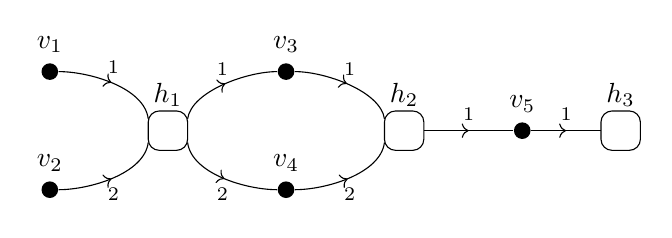
\begin{tikzpicture}
			\node[circle,fill=black,inner sep=0pt,minimum size=6pt,label=above:{$v_1$}] (A) at (0,0) {};
			\node[circle,fill=black,inner sep=0pt,minimum size=6pt,label=above:{$v_2$}] (B) at (0,-1.5) {};
			\node[circle,fill=black,inner sep=0pt,minimum size=6pt,label=above:{$v_3$}] (C) at (3,0) {};
			\node[circle,fill=black,inner sep=0pt,minimum size=6pt,label=above:{$v_4$}] (D) at (3,-1.5) {};
			\node[circle,fill=black,inner sep=0pt,minimum size=6pt,label=above:{$v_5$}] (E) at (6,-0.75) {};
			\draw[rounded corners] (1.25, -1) rectangle (1.75, -0.5) {};
			\draw[->-=.5](4.75,-0.75)--(E)node[pos=0.5, above,font=\fontsize{7}{0}\selectfont]{$1$};
			\draw[->-=.5](E)--(7,-0.75)node[pos=0.5, above,font=\fontsize{7}{0}\selectfont]{$1$};
			\draw[rounded corners] (4.25, -1) rectangle (4.75, -0.5) {};
			\node at (4.5, -0.3){$h_2$};
			\node at (1.5, -0.3){$h_1$};
			\node at (7.25, -0.3){$h_3$};
			\draw[rounded corners] (7, -1) rectangle (7.5, -0.5) {};
			\draw(A)[->-=.5]..controls(0.5,0)and(1.2,-0.2)..(1.25,-0.6)node[pos=0.5, above,font=\fontsize{7}{0}\selectfont]{$1$};
			\draw(B)[->-=.5]..controls(0.5,-1.5)and(1.2,-1.3)..(1.25,-0.9)node[pos=0.5, below,font=\fontsize{7}{0}\selectfont]{$2$};
			
			\draw(C)[->-=.5]..controls(3.5,0)and(4.2,-0.25)..(4.25,-0.6)node[pos=0.5, above,font=\fontsize{7}{0}\selectfont]{$1$};
			\draw(D)[->-=.5]..controls(3.5,-1.5)and(4.2,-1.3)..(4.25,-0.9)node[pos=0.5, below,font=\fontsize{7}{0}\selectfont]{$2$};
			
			\draw[->-=.5](1.75,-0.9)..controls(1.8,-1.3)and(2.5,-1.5)..(D)node[pos=0.5, below,font=\fontsize{7}{0}\selectfont]{$2$};
			\draw[->-=.5] (1.75,-0.6)..controls(1.8,-0.25)and(2.5,0)..(C) node[pos=0.5, above,font=\fontsize{7}{0}\selectfont]{$1$};
		\end{tikzpicture}
	\end{center}
\end{example}

\begin{example}\label[example]{exa_21} Let $V_{\mathcal{G}}$ be as in the previous example and $E_{\mathcal{G}}=\{h_1, h_2, h_3\}$.	Then we define
	\[\begin{matrix}
		A && s_{\mathcal{G}}(h_1)\colon 0\to V_{\mathcal{G}}  & s_{\mathcal{G}}(h_1)=?_{V_\mathcal{G}} && s_{\mathcal{G}}(h_2)\colon 2\to V_{\mathcal{G}} & \begin{matrix}
			0 \mapsto v_1\\
			1\mapsto v_2
		\end{matrix}&& s_{\mathcal{G}}(h_3)\colon 2\to V_{\mathcal{G}} & \begin{matrix} 
			0 \mapsto v_1\\
			1\mapsto v_4	
		\end{matrix}\\
			B && t_{\mathcal{G}}(h_1)\colon 1\to V_{\mathcal{G}} & 
		0 \mapsto v_1 && 		t_{\mathcal{G}}(h_2)\colon 1\to V_{\mathcal{G}} & 0\mapsto v_3 &&   t_{\mathcal{G}}(h_3)\colon 1\to V_{\mathcal{G}} & 1\mapsto v_5
	\end{matrix}\]
	
	Now we can depict $\mathcal{G}$ as
	\begin{center}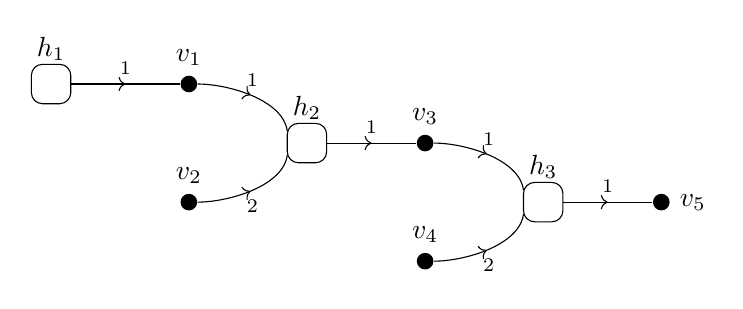
\begin{tikzpicture}
			\node[circle,fill=black,inner sep=0pt,minimum size=6pt,label=above:{$v_1$}] (A) at (0,0) {};
			\node[circle,fill=black,inner sep=0pt,minimum size=6pt,label=above:{$v_2$}] (B) at (0,-1.5) {};
			\node[circle,fill=black,inner sep=0pt,minimum size=6pt,label=above:{$v_3$}] (C) at (3,-0.75) {};
			\node[circle,fill=black,inner sep=0pt,minimum size=6pt,label=above:{$v_4$}] (D) at (3,-2.25) {};
			\node[circle,fill=black,inner sep=0pt,minimum size=6pt,label=right:{$v_5$}] (E) at (6,-1.5) {};
			\draw[->-=.5] (1.75,-0.75)--(C)node[pos=0.5, above,font=\fontsize{7}{0}\selectfont]{$1$};
			\draw[rounded corners] (1.25, -1) rectangle (1.75, -0.5) {};
			\draw[->-=.5] (4.75,-1.5)--(E)node[pos=0.5, above,font=\fontsize{7}{0}\selectfont]{$1$};
			\draw[->-=.5] (-1.5,0)--(A)node[pos=0.5, above,font=\fontsize{7}{0}\selectfont]{$1$};
			\draw[rounded corners] (4.25, -1.75) rectangle (4.75, -1.25) {};
			\node at (4.5, -1.05){$h_3$};
			\node at (1.5, -0.3){$h_2$};
			\node at (-1.75, 0.45){$h_1$};
			\draw[rounded corners] (-2, -0.25) rectangle (-1.5, 0.25) {};
			\draw[->-=.5] (A)..controls(0.5,0)and(1.2,-0.2)..(1.25,-0.6)node[pos=0.5, above,font=\fontsize{7}{0}\selectfont]{$1$};
			\draw[->-=.5] (B)..controls(0.5,-1.5)and(1.2,-1.3)..(1.25,-0.9)node[pos=0.5, below,font=\fontsize{7}{0}\selectfont]{$2$};
			
			\draw[->-=.5] (C)..controls(3.5,-0.75)and(4.2,-0.95)..(4.25,-1.35)node[pos=0.5, above,font=\fontsize{7}{0}\selectfont]{$1$};
			\draw[->-=.5] (D)..controls(3.5,-2.25)and(4.2,-2.05)..(4.25,-1.65)node[pos=0.5, below,font=\fontsize{7}{0}\selectfont]{$2$};
		\end{tikzpicture}
	\end{center}
\end{example}
\fi

\commentato{
\begin{example}\label[example]{exa_2}
	Let $V_\mathcal{G} = \{v_1, v_2, v_3, v_4, v_5\}$, and $E_\mathcal{G} = \{h_1, h_2, h_3, h_4\}$. Then we define:
	\[\begin{matrix}
		s_{\mathcal{G}}(h_1)\colon 0\to V_{\mathcal{G}} & s_{\mathcal{G}}(h_1)=?_{V_\mathcal{G}} &&
		s_{\mathcal{G}}(h_2)\colon 0\to V_{\mathcal{G}} & s_{\mathcal{G}}(h_2)=?_{V_\mathcal{G}}\\
		s_{\mathcal{G}}(h_3)\colon 2\to V_{\mathcal{G}} & \begin{matrix} 
					0 \mapsto v_1\\
					1\mapsto v_2
				\end{matrix}&& s_{\mathcal{G}}(h_4)\colon 2 \to V_\mathcal{G} & \begin{matrix}
					0 \mapsto v_3\\
					1\mapsto v_2
				\end{matrix}\\
		t_{\mathcal{G}}(h_1)\colon 1\to V_{\mathcal{G}} & 0 \mapsto v_1 &&
		t_{\mathcal{G}}(h_2)\colon 1\to V_{\mathcal{G}} & 0\mapsto v_3\\
		t_{\mathcal{G}}(h_3)\colon 1\to V_{\mathcal{G}} & 1\mapsto v_3 &&
		t_\mathcal{G}(h_4)\colon 1 \to V_\mathcal{G} & 0 \mapsto v_4
	\end{matrix}\]

	Now, we can depict $\mathcal{G}$ as

	\begin{center}
		        \begin{tikzpicture}
                \begin{pgfonlayer}{nodelayer}
                        \node[style=none] (lab1) at (-1.8, 0.8) {$h_1$};
                        \node[style=small box] (h1) at (-1.8, 0.3) {};
                        \node[style=small box] (2) at (-1.8, -0.5) {};
                        \node[style=none] (lab2) at (-1.8, -1.0) {$h_2$};
                        \node[style=none] (h1b) at (-1.8, 0.3) {};
                        \node[style=none] (th2) at (-0.3, 0.3) {};
                        \node[style=none] (bh2) at (-0.3, -0.3) {};
                        \node[style=none] (h2b) at (0, 0) {};
                        \node[style=none] (th3) at (1.5, 0){};
                        \node[style=none] (bh3) at (1.5, -0.6){};
                        \node[style=none] (h3c) at (1.8, -0.3){};
                        \node[style=none] (2c) at (-1.8, -0.5){};
                        \node[style=none] (lab3) at (0, 0.8) {$h_3$};
                        \node[style=medium box] (h2) at (0, 0) {};
                        \node[style=none] (lab4) at (1.8, 0.5) {$h_4$};
                        \node[style=medium box] (h3) at (1.8, -0.3) {};
                        \node[style=none](labv2) at (-0.9, -0.9) {$v_2$};
                        \node[style=node] (v2) at (-0.9, -0.5) {};
                        \node[style=none] (labv1) at (-0.9, 0.7) {$v_1$};
                        \node[style=node] (v1) at (-0.9, 0.3) {};
                        \node[style=none] (labv3) at (0.9, 0.4) {$v_3$};
                        \node[style=node] (v3) at (0.9, 0) {};
                        \node[style=none] (labv4) at (2.7, 0.1) {$v_4$};
                        \node[style=node] (v4) at (2.7, -0.3) {};
                \end{pgfonlayer}
                \begin{pgfonlayer}{edgelayer}
                        \draw[style=diredge] (h1b.center) to (v1);
                        \draw[style=diredge] (v1) to (th2.center);
                        \draw[style=diredge] (2c.center) to (v2);
                        \draw[style=diredge, in=180, out=30] (v2) to (bh2.center);
                        \draw[style=diredge] (v3) to (th3.center);
                        \draw[style=diredge] (h3c.center) to (v4);
                        \draw[style=diredge] (h2b.center) to (v3);
                        \draw[style=diredge,in=180, out=-30](v2) to (bh3);
                \end{pgfonlayer}
        \end{tikzpicture}
\end{center}

\end{example}
}

\begin{remark}\label{rem:functor}
	It is worth to point out, as first noted in \cite{bonchi2022string}, that $\hyp$ is equivalent to a category of functors. 
	%
	Indeed, consider the category $\catname{H}$ in which the set of objects is given by $ (\mathbb{N}\times \mathbb{N}) \cup \{\bullet\}$ and arrows are given by the identities $\id{k,l}$, $\id{\bullet}$ and exactly $k+l$ arrows $f_i\colon (k,l)\rightarrow \bullet$, where $i$ ranges from $0$ to $k+l-1$. 
	%
	The functors $\catname{H}\to \Set$ corresponds exactly to hypergaphs: nodes correspond to the image of $\bullet$ while the set of hyperedges with source of length $k$ and target of length $l$ corresponds to the image of $(k,l)$ (see \cite{CastelnovoGM24}).
\end{remark}

In particular, \Cref{rem:functor} entails the following result. 

\begin{proposition}\label{prop:cocomp}
	$\hyp$ has all limits and colimits.
\end{proposition}

\iffalse
\subsubsection{$\hyp$ as a category of functors}

Following \cite{bonchi2022string}, we can present $\hyp$ as a category of functor over a suitable category.

\begin{definition}Let $\catname{H}$ be the category such that
	\begin{itemize}
		\item the set of objects is $ (\mathbb{N}\times \mathbb{N}) \cup \{\bullet\}$;
		\item arrows are given by the identities $\id{k,l}$ and $\id{\bullet}$ and exactly $k+l$ arrows $f_i\colon (k,l)\rightarrow \bullet$, where $i$ ranges from $0$ to $k+l-1$;
		\item composition is defined by putting
		%\begin{equation*}
			$f_i=f_i\circ \id{k,l}$ and $f_i = \id{\bullet}\circ f_i$
		%\end{equation*}
		for every $f_i\colon (k,l)\rightarrow \bullet$.
	\end{itemize}
\end{definition}

The idea is that for every functor $F\colon \catname{H}\to \catname{Set}$ we can define
\[E_F:=\sum_{k,l\in \mathbb{N}}F(k,l)\]
%
Now, for every $k$, $l$, $i$ and $j$ in $\mathbb{N}$ with $i< k$ and $j< l$ we define $s^F_{k,l}\colon F(k,l)\to F(\bullet)^k$ and  $t^F_{k,l}\colon F(k,l)\to F(\bullet)^l$ as the unique arrows fitting in the diagrams below, where the vertical arrows are the projections
\[\xymatrix{F(k,l)  \ar@{.>}[r]^{s^F_{k,l}} \ar[dr]_{F(f_i)}& F(\bullet)^{k} \ar[d]^{\pi^F_{k,i}} & F(k,l) \ar@{.>}[r]^{t^F_{k,l}} \ar[dr]_{F(f_{k+j})} & F(\bullet)^{l} \ar[d]^{\pi^F_{l,j}} \\ & F(\bullet) && F(\bullet)}\]
%
In turn, these arrows allow us to consider
$s_F, t_F\colon E_F\rightrightarrows F(\bullet)^{\star}$ as the unique arrows fitting in the diagrams below, where the vertical arrows are coprojections
\[\xymatrix{F(k,l) \ar[d]_{a^F_{k,l}}  \ar[r]^{s^{F}_{k,l}}& F(\bullet)^{k} \ar[d]^{b^F_{k}} & F(k,l) \ar[d]_{a^F_{k,l}}  \ar[r]^{t^{F}_{k,l}}& F(\bullet)^{l} \ar[d]^{b^F_{l}}\\ E_F \ar@{.>}[r]_-{s_F}& F(\bullet)^\star & E_F \ar@{.>}[r]_-{t_F}& F(\bullet)^\star}\]

Let $\mathcal{G}_F$ be the resulting hypergraph. One can now show that  sending $F$ to $\mathcal{G}_F$ can be extended to an equivalence $\mathcal{G}_{-}\colon \Set^{\catname{H}}\to \hyp$ (see \cite{castelnovo2023thesis,CastelnovoGM24} for details).


\begin{proposition}
	$\hyp$ is equivalent to the category $\Set^{\catname{H}}$.
\end{proposition}
\fi

\subsubsection{Labelling hypergraph with an algebraic signature}\label{sssect:hyp_alg_sign}

Our interest for hypergraphs stems from their use as a graphical representation of algebraic terms. We thus need a way to label hyperedges with symbols taken from a signature.

\noindent
\begin{minipage}[l]{.73\linewidth}
\begin{definition}
An \emph{algebraic signature} $\Sigma$ is a pair $(O_\Sigma, \ari_\Sigma)$ given by a \emph{set of operations} $O_\Sigma$ and an \emph{arity function} $\ari_\Sigma\colon O_\Sigma \to \mathbb{N}$. 
%
We define the \emph{hypergraph $\mathcal{G}_\Sigma$ associated with $\Sigma$} taking $O_\Sigma$ as set of hyperedges, $\{1\}$ as set of nodes, so that $\{1\}^\star$ is $\mathbb{N}$, $\ari_\sigma$ as the source function and $\delta_1$ as target function, which always picks the element $1$. The category $\hyps$ of \emph{algebraically labelled hypergraphs} is the slice category $\hyp/\mathcal{G}^\Sigma$.
\end{definition}

\iffalse
\todo{Decidere se tenere questo esempio}

\begin{example}\label[example]{exa_3} Let $\Sigma=(O_\Sigma, \ari_\Sigma)$ be an algebraic signature in $\Set$. This simply amount to a set of \emph{operations} with an associated natural number, called \emph{arity}. 	For instance let $\Sigma_G$ be the signature of groups, then $\mathcal{G}^{\Sigma_G}$ can be depicted as the picture aside.
	\begin{center}
		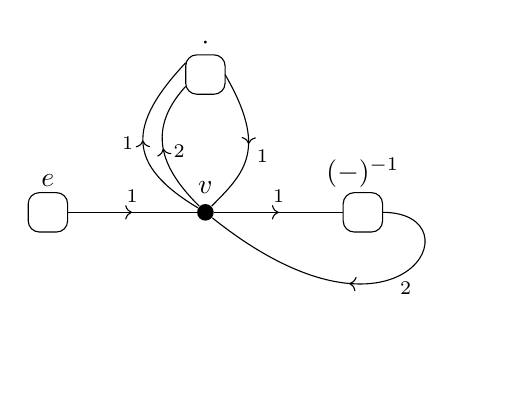
\begin{tikzpicture}
			\node[circle,fill=black,inner sep=0pt,minimum size=6pt,label=above:{$v$}] (V) at (0,0) {};
			\node(E)at(-2, 0.4){$e$};
			\node(M)at(0, 2.15){$\cdot$};
			\node(I)at(2, 0.5){$(-)^{-1}$};
			\draw[->-=.5](-1.75,0)--(V)node[pos=0.5, above,font=\fontsize{7}{0}\selectfont]{$1$};
			\draw[->-=.5](V)..controls(-0.5,0.5)and(-0.8,1)..(-0.25,1.6)node[pos=0.5, right,font=\fontsize{7}{0}\selectfont]{$2$};
			\draw[->-=.5](V)..controls(-1,0.6)and(-1,1.1)..(-0.25,1.9)node[pos=0.5, left,font=\fontsize{7}{0}\selectfont]{$1$};
			\draw[->-=.5](0.25,1.75)..controls(0.8,0.8)and(0.5,0.5)..(V)node[pos=0.5, right,font=\fontsize{7}{0}\selectfont]{$1$};
			\draw[->-=.5](V)--(1.75,0)node[pos=0.5, above,font=\fontsize{7}{0}\selectfont]{$1$};
			\draw[->-=.5](2.25,0)..controls(3.5,0)and(2.5,-2)..(V)node[pos=0.5, below,font=\fontsize{7}{0}\selectfont]{$2$};
			\draw[rounded corners] (-2.25, -0.25) rectangle (-1.75, 0.25) {};
			\draw[rounded corners] (-0.25, 1.5) rectangle (0.25, 2) {};
			\draw[rounded corners] (2.25, -0.25) rectangle (1.75, 0.25) {};
		\end{tikzpicture}
	\end{center}
\end{example}\fi

\begin{example}\label[example]{exa_3}
	Let $\Sigma = (O_\Sigma, \ari_\Sigma)$ be the signature with $O_\Sigma =  \mathbb{N} \uplus A \uplus \{*, /\}$, 
	where $n$ stands for any natural number and $a$ for any element in $A$, both sets of constants, and
	%so that $\ari_\Sigma(n)=\ari_\Sigma(a) = 0$, 
	$\ari_\Sigma(*) = \ari_\Sigma(/) = 2$. Then the hypergraph $\mathcal{G}^\Sigma$ is depicted as the picture aside.
\end{example}
\end{minipage}
%\begin{center}
\hfill
\begin{minipage}[r]{.22\linewidth}
\begin{tikzpicture}
        \begin{pgfonlayer}{nodelayer}
                \node[style=node] (v) at (0, 0){};
                \node[style=none] (vlab) at (0, -0.4){$v$};
                
                \node[style=small box] (n) at (-1.8, 0.4) {};
                \node[style=none] (nlab) at (-1.8, 0.9) {$n$};
                \node[style=none] (nattach) at (-1.6, 0.4) {};

                \node[style=small box] (const) at (-1.8, -0.4) {};
                \node[style=none] (constlab) at (-1.8, -0.9){$a$};
                \node[style=none] (constattach) at (-1.6, -0.4){};

                \node[style=medium box] (times) at (0, 1.8) {};
                \node[style=none] (timeslab) at (0, 2.6) {$*$};
                \node[style=none] (timesin1) at (-0.3, 2.1) {};
                \node[style=none] (timesin2) at (-0.3, 1.5) {};
                \node[style=none] (timesout) at (0.2, 1.8){};

                \node[style=medium box] (div) at (0, -1.8) {};
                \node[style=none] (divlab) at (0, -2.6) {$/$};
                \node[style=none] (divin1) at (-0.3, -2.1) {};
                \node[style=none] (divin2) at (-0.3, -1.5) {};
                \node[style=none] (divout) at (0.2, -1.8){};
        \end{pgfonlayer}

        \begin{pgfonlayer}{edgelayer}
                \draw[style=diredge, in=180, out= 112.5] (v) to (timesin2.center); 
                \draw[style=diredge,out=135, in= 180] (v) to (timesin1.center);
                \draw[style=diredge,in=165, out=0] (nattach.center) to (v);
                
                \draw[style=diredge,out=0, in=-165] (constattach.center) to (v);
                \draw[style=diredge,in=180, out= -112.5] (v) to (divin2.center); 
                \draw[style=diredge,out=-135, in= 180] (v) to (divin1.center);

                \draw[style=diredge, in=30, out=0] (timesout.center) to (v);
                \draw[style=diredge, in=-30, out=0] (divout.center) to (v);
        \end{pgfonlayer}
\end{tikzpicture}
\end{minipage}

\Cref{cor:mono} and \Cref{thm:slice-functors} give us immediately an adhesivity result for $\hyp_{\Sigma}$ and a characterisation of monos in it.

\begin{proposition}\label[proposition]{prop:mono} Let $\Sigma$ be an algebraic signature. Then it holds
	\begin{enumerate}
		\item an arrow $(h,k)$ in $\hyp_{\Sigma}$ is a mono if and only if $h$ and $k$ are injective;
		\item $\hyp_{\Sigma}$ is an adhesive category. 
	\end{enumerate}
\end{proposition}

\noindent 
\parbox{10.8cm}{\begin{remark}\label[remark]{rem:label}	
Let $\mathcal{H}=(E, V, s, t)$ be an hypergraph, by definition we know that $U_{\hyp}(\mathcal{G}^{\Sigma})$ is the terminal object $1$, so an arrow $\mathcal{H}\rightarrow \mathcal{G}^{\Sigma}$, is determined by a morphism $h\colon E_\mathcal{H}\to O_\Sigma$  making the two squares on the right commutative (cfr.~\Cref{rem:length}).

\hspace{10pt}Now, consider a coprojection $v_n\colon V^n_\mathcal{H}\to  V^\star_{\mathcal{H}}$.  The second diagram above entails that $t_{\mathcal{H}}$ factors via the inclusion $v_1\colon V_{\mathcal{H}}\to V^{\star}$ of words of length $1$, i.e. $t_{\mathcal{H}}=v_1\circ \tau_{\mathcal{H}}$ for some $\tau_{\mathcal{H}}\colon E_{\mathcal{H}}\to V_{\mathcal{H}}$.
\end{remark}} \hfill \parbox{3cm}{\xymatrix@R=15pt{E_{\mathcal{H}} \ar[r]_{h}\ar[d]_{s_{\mathcal{H}}} & O_\Sigma \ar[d]^{\ari_\Sigma} \\ V_{\mathcal{H}} \ar[r]^{\lgh_{V_{\mathcal{H}}}} & \mathbb{N}} \hspace{1pt}\\ \xymatrix@R=15pt{E_{\mathcal{H}} \ar[r]_{h}\ar[d]_{t_{\mathcal{H}}} & O_\Sigma \ar[d]^{\ari_\Sigma}\\ V_{\mathcal{H}}\ar[r]^{\lgh_{V_{\mathcal{H}}}} & \mathbb{N}}}

$\hyp_{\Sigma}$, has a forgetful functor $U_{\Sigma}\colon \hyp_{\Sigma}\to \X$ which sends $(h,k)\colon \mathcal{H}\to \mathcal{G}^{\Sigma}$ to $U_{\X}(\mathcal{H}$). Now, $U_{\hyp}(\mathcal{G}^{\Sigma})=1$ thus, for every set $X$ we can define $\Delta_{\Sigma}(X)\colon \Delta_{\X}(X)\to \mathcal{G}^{\Sigma}$  as $(?_{O_\Sigma}, !_{X})$. It is straightforward to see that in this way we get a left adjoint to $U_\Sigma$.

\begin{proposition} $U_\Sigma$
	has a left adjoint $\Delta_\Sigma$.
\end{proposition}
\iffalse 
\begin{proof}Let $(h, !_{V_\mathcal{H}})\colon \mathcal{H}\to \mathcal{G}^{\Sigma}$ be an object of $\hyp_{\Sigma}$, and suppose that there exists $f\colon X\to U_{\Sigma}(\mathcal{H})$. Since, $U_{\Sigma}(\mathcal{H})=U_{\X}(\mathcal{H})$ and the identity is the unit of $\Delta_\hyp \dashv U_{\hyp}$, we get a morphism $(?_{E_{\mathcal{H}}},f)\colon \Delta_{\X}(X)\to \mathcal{H}$ of $\hyp$. And then the thesis follows since we have
	\[
	(h, !_{V_{\mathcal{{H}}}})\circ (?_{E_{\mathcal{H}}}, f)=(h\circ ?_{E_{\mathcal{H}}}, !_{V_{\mathcal{{H}}}}\circ f)=(?_{0_{\Sigma}}, !_{X})=\Delta_{\hyp}(X)\]
%and the thesis follow.   
\end{proof}
 

\todo{anche questo forse val la pena toglierlo}
\todo{presentarlo come string diagram e magari prendere la segnatura de un esempio egg}

\begin{example}\label[example]{lab_1}
	The simplest example is given by the identity $\id{\mathcal{G}^\Sigma}\colon \mathcal{G}^\Sigma\rightarrow \mathcal{G}^{\Sigma}$. If $\Sigma$ is the signature of groups $\Sigma_G$ we get 
	\begin{center}
		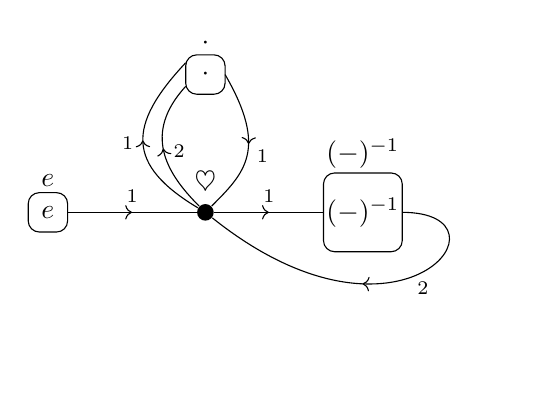
\begin{tikzpicture}
			\node[circle,fill=black,inner sep=0pt,minimum size=6pt,label=above:{$\heartsuit$}] (V) at (0,0) {};
			\node(E)at(-2, 0.4){$e$};
			\node(M)at(0, 2.15){$\cdot$};
			\node(I)at(2, 0.75){$(-)^{-1}$};
			
			\node(E')at(-2, 0){$e$};
			\node(M')at(0, 1.75){$\cdot$};
			\node(I')at(2, 0){$(-)^{-1}$};
			\draw[->-=.5](-1.75,0)--(V)node[pos=0.5, above,font=\fontsize{7}{0}\selectfont]{$1$};
			\draw[->-=.5](V)..controls(-0.5,0.5)and(-0.8,1)..(-0.25,1.6)node[pos=0.5, right,font=\fontsize{7}{0}\selectfont]{$2$};
			\draw[->-=.5](V)..controls(-1,0.6)and(-1,1.1)..(-0.25,1.9)node[pos=0.5, left,font=\fontsize{7}{0}\selectfont]{$1$};
			\draw[->-=.5](0.25,1.75)..controls(0.8,0.8)and(0.5,0.5)..(V)node[pos=0.5, right,font=\fontsize{7}{0}\selectfont]{$1$};
			\draw[->-=.5](V)--(1.5,0)node[pos=0.5, above,font=\fontsize{7}{0}\selectfont]{$1$};
			\draw[->-=.5](2.5,0)..controls(4,0)and(2.5,-2)..(V)node[pos=0.5, below,font=\fontsize{7}{0}\selectfont]{$2$};
			\draw[rounded corners] (-2.25, -0.25) rectangle (-1.75, 0.25) {};
			\draw[rounded corners] (-0.25, 1.5) rectangle (0.25, 2) {};
			\draw[rounded corners] (2.5, -0.5) rectangle (1.5, 0.5) {};
		\end{tikzpicture}
	\end{center}
\end{example}


\todo{Decidere se tenere questo esempio (io direi di no)}
\fi

We will extend our graphical notation of hypergraphs to labeled ones putting the label of an hyperedge $h$ inside its corresponding square.

\begin{example}\label[example]{lab_2}
	Consider again $\Sigma$ the signature of \Cref{exa_3}, then the hypergraph $\mathcal{G}$ of \Cref{exa_2} can be labeled by a morphism
	$(l, !_{V_\mathcal{G}}): \mathcal{G} \to \mathcal{G}^\Sigma$ that is characterised by the image of the edges. 
	If $l(h(1) = a$, $l(h_2) = 2$, $l(h_3) = *$, and $l(h_4) = /$, we represent it visually 
	by putting the identifiers of the edges in  $\mathcal{G}^\Sigma$ inside the boxes representing the edges of $\mathcal{G}$,
	and removing the idetifiers on the nodes and edges of the latter, as
		\begin{center}
		\begin{tikzpicture}
			\begin{pgfonlayer}{nodelayer}
				\node[style=none] (lab1) at (-1.8, 0.8) {};
				\node[style=small box] (h1) at (-1.8, 0.3) {$a$};
				\node[style=small box] (2) at (-1.8, -0.5) {$2$};
				\node[style=none] (lab2) at (-1.8, -1.0) {};
				\node[style=none] (h1b) at (-1.8, 0.3) {};
				\node[style=none] (th2) at (0, 0.3) {};
				\node[style=none] (bh2) at (0, -0.3) {};
				\node[style=none] (h2b) at (0, 0) {};
				\node[style=none] (th3) at (1.8, 0){};
				\node[style=none] (bh3) at (1.8, -0.6){};
				\node[style=none] (h3c) at (1.8, -0.3){};
				\node[style=none] (2c) at (-1.8, -0.5){};
				\node[style=none] (lab3) at (0, 0.8) {};
				\node[style=medium box] (h2) at (0, 0) {$*$};
				\node[style=none] (lab4) at (1.8, 0.5) {};
				\node[style=medium box] (h3) at (1.8, -0.3) {$/$};
				\node[style=none](labv2) at (-0.9, -0.9) {};
				\node[style=node] (v2) at (-0.9, -0.5) {};
				\node[style=none] (labv1) at (-0.9, 0.7) {};
				\node[style=node] (v1) at (-0.9, 0.3) {};
				\node[style=none] (labv3) at (0.9, 0.4) {};
				\node[style=node] (v3) at (0.9, 0) {};
				\node[style=none] (labv4) at (2.7, 0.1) {};
				\node[style=node] (v4) at (2.7, -0.3) {};
			\end{pgfonlayer}
			\begin{pgfonlayer}{edgelayer}
				\draw (h1b.center) to (th2.center);
				\draw (2c.center) to (v2);
				\draw[in=180, out=30] (v2) to (bh2.center);
				\draw (h2b.center) to (th3.center);
				\draw (v4) to (h3c.center);
				%\draw (h3c) to (v4);
				\draw[in=180, out=-30](v2) to (bh3);
			\end{pgfonlayer}
        	\end{tikzpicture}
	\end{center}
%
	\iffalse
	\begin{center}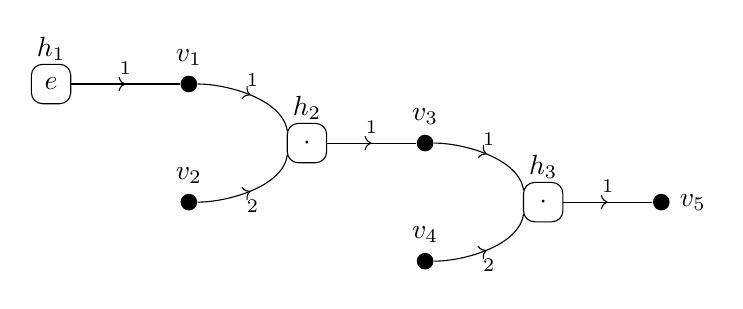
\begin{tikzpicture}
			\node[circle,fill=black,inner sep=0pt,minimum size=6pt,label=above:{$v_1$}] (A) at (0,0) {};
			\node[circle,fill=black,inner sep=0pt,minimum size=6pt,label=above:{$v_2$}] (B) at (0,-1.5) {};
			\node[circle,fill=black,inner sep=0pt,minimum size=6pt,label=above:{$v_3$}] (C) at (3,-0.75) {};
			\node[circle,fill=black,inner sep=0pt,minimum size=6pt,label=above:{$v_4$}] (D) at (3,-2.25) {};
			\node[circle,fill=black,inner sep=0pt,minimum size=6pt,label=right:{$v_5$}] (E) at (6,-1.5) {};
			\draw[->-=.5] (1.75,-0.75)--(C)node[pos=0.5, above,font=\fontsize{7}{0}\selectfont]{$1$};
			\draw[rounded corners] (1.25, -1) rectangle (1.75, -0.5) {};
			\draw[->-=.5] (4.75,-1.5)--(E)node[pos=0.5, above,font=\fontsize{7}{0}\selectfont]{$1$};
			\draw[->-=.5] (-1.5,0)--(A)node[pos=0.5, above,font=\fontsize{7}{0}\selectfont]{$1$};
			\draw[rounded corners] (4.25, -1.75) rectangle (4.75, -1.25) {};
			\node at (4.5, -1.05){$h_3$};
			\node at (1.5, -0.3){$h_2$};
			\node at (-1.75, 0.45){$h_1$};
			\draw[rounded corners] (-2, -0.25) rectangle (-1.5, 0.25) {};
			\draw[->-=.5] (A)..controls(0.5,0)and(1.2,-0.2)..(1.25,-0.6)node[pos=0.5, above,font=\fontsize{7}{0}\selectfont]{$1$};
			\draw[->-=.5] (B)..controls(0.5,-1.5)and(1.2,-1.3)..(1.25,-0.9)node[pos=0.5, below,font=\fontsize{7}{0}\selectfont]{$2$};
			
			\draw[->-=.5] (C)..controls(3.5,-0.75)and(4.2,-0.95)..(4.25,-1.35)node[pos=0.5, above,font=\fontsize{7}{0}\selectfont]{$1$};
			\draw[->-=.5] (D)..controls(3.5,-2.25)and(4.2,-2.05)..(4.25,-1.65)node[pos=0.5, below,font=\fontsize{7}{0}\selectfont]{$2$};
			
			\node at (-1.75,0) {$e$};
			\node at (1.5,-0.75) {$\cdot$};
			\node at (4.5,-1.5) {$\cdot$};
		\end{tikzpicture}
	\end{center}\fi
\end{example}


\subsection{Term Graphs}
\todo{a very nice introduction}

Let us start using labelled hypergraphs to define term graphs.

\begin{definition}\label[definition]{def:tg}\index{term graph}
	Given an algebraic signature $\Sigma$, we say that a labelled hypergraph $(l, !_{V_\mathcal{G}})\colon \mathcal{G}\to \mathcal{G}^{\Sigma}$ is a \emph{term graph} if $t_\mathcal{G}$ is a mono. We define $\tg$ to be the full subcategory of $\hyp_{\Sigma}$ and denote by $I_\Sigma$ the inclusion. Restricting $U_\Sigma\colon \hyp_{\Sigma}\to \catname{Set}$ we get a forgetful functor $U_{\tg}\colon \tg\to \catname{Set}$.
\end{definition}


\begin{remark}\label[remark]{rem:mono2}By \Cref{rem:label}, we know that if $\mathcal{G}$ is a term graph then $t_{\mathcal{G}}=v_1\circ \tau_{\mathcal{G}}$, where $v_1$ is the coprojection of $V_{\mathcal{G}}$ into $V^\star_{\mathcal{G}}$.  Notice that since $t_{\mathcal{G}}$ is a mono then $\tau_{\mathcal{G}}$ is a mono too.
\end{remark}

We now examine some properties of $\tg$, in order to study its adhesivity properties.

\begin{proposition}\label[proposition]{term:left}The forgetful functor $U_{\tg}$ has a left adjoint $\Delta_{\tg}$.
\end{proposition}
\commentato{
\begin{proof}
	This follows noticing that $\Delta_{\Sigma}(X)$ is a term graph for every object $X$.
\end{proof}}

We can list some other categorical properties of $\tg$.


\begin{proposition}
Let $\Sigma$ be an algebraic signature. Then it holds
\begin{enumerate}
	\item if  $(i,j)\colon \mathcal{H}\to \mathcal{G}$ is a mono between  $(l, !_{V_\mathcal{G}})\colon \mathcal{G}\to \mathcal{G}^{\Sigma}$ and $(l', !_{V_\mathcal{H}})\colon \mathcal{H}\to \mathcal{G}^{\Sigma}$ in $\hyp_\Sigma$ and the latter is in $\tg$, then also the former is in $\tg$
	\item $\tg$ has equalizers, binary products and pullbacks and they are created by $I_\Sigma$.
\end{enumerate}
\end{proposition}

\begin{remark}
	$\tg$ in general does not have terminal objects. 
	%Consider an algebraic signature in $\Set$. 
	Since $U_{\tg}$ preserves limits, if a terminal object exists it must have the singleton as set of nodes, therefore the set of hyperedges must be empty or a singleton. 
	Hence, for a counterexample, it suffices to take as signature the one given by two operations $a$ and $b$, both of arity $0$.
	$\tg$ is not an adhesive category, either. 
	In particular, as noted in e.g.~\cite{CastelnovoGM24}, 
	 it does not have pushouts along all monos. 
\end{remark}
	
\commentato{
\begin{remark}
	$\tg$ in general does not have terminal objects. Consider an algebraic signature in $\Set$. Since $U_{\tg}$ preserves limits, if a terminal object exists it must have the singleton as set of nodes, therefore the set of hyperedges must be empty or a singleton $\{h\}$. Hence, for a counterexaqmple it suffices to take as signature the one given by two operations $a$ and $b$, both of arity $0$; we have three term graphs with only one node $v$: $\Delta_{\tg{\Sigma}}(\{v\})$, $(l_a, !_{V_{\mathcal{G}}})\colon \mathcal{G}_a\to \mathcal{G}^{\Sigma}$ and $(l_b, !_{V_{\mathcal{G}}})\colon \mathcal{G}_b\to \mathcal{G}^{\Sigma}$.
	\begin{center}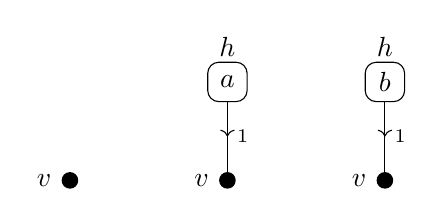
\begin{tikzpicture}
			
			\node[circle,fill=black,inner sep=0pt,minimum size=6pt,label=left:{$v$}] (V) at (5,0) {};
			\node[circle,fill=black,inner sep=0pt,minimum size=6pt,label=left:{$v$}] (U) at (3,0) {};
			\node at(5,1.25){$a$};	
			\node at(5,1.7){$h$};	
			
			\draw[->-=.5](5,1)--(V)node[pos=0.5, right,font=\fontsize{7}{0}\selectfont]{$1$};
			
			\draw[rounded corners] (4.75, 1) rectangle (5.25, 1.5) {};
			
			
			\node[circle,fill=black,inner sep=0pt,minimum size=6pt,label=left:{$v$}] (V) at (7,0) {};
			
			\node at(7,1.25){$b$};	
			\node at(7,1.7){$h$};	
			
			\draw[->-=.5](7,1)--(V)node[pos=0.5, right,font=\fontsize{7}{0}\selectfont]{$1$};
			
			\draw[rounded corners] (6.75, 1) rectangle (7.25, 1.5) {};
			
		\end{tikzpicture}
	\end{center}
	There are no morphisms in $\tg$ between the last two and from the last two to the first one, therefore none of them can be terminal.
\end{remark}

\begin{remark}
	$\tg$ is not an adhesive category. In particular it does not have pushouts along all monos. For instance, if we take the three term graphs of the previous remark, then have two arrows
	$(?_{\{h\}}, \id{\{v\}})\colon \Delta_{\tg}(\{v\})\to (l_a, !_{V_{\mathcal{G}_a}})$ and $(?_{\{h\}}, \id{\{v\}})\colon \Delta_{\tg}(\{v\})\to (l_b, !_{V_{\mathcal{G}_a}})$ which cannot be completed to a square. Indeed if $(q, !_{V_\mathcal{H}})\colon \mathcal{H}\to \mathcal{G}^\Sigma$ is another term graph with $(g_E, g_V)\colon (l_a, !_{V_{\mathcal{G}}})\to (q, !_{V_\mathcal{H}})$ and $(k_E, k_V)\colon (l_a, !_{V_{\mathcal{G}}})\to (q, !_{V_\mathcal{H}})$  such that 
	\[(g_E, g_V)\circ (?_{\{h\}}, \id{\{v\}}) = (k_E, k_V)\circ (?_{\{h\}}, \id{\{v\}})\]
	then $g_V=k_V$ and
	\[t_{\mathcal{H}}(g_E(h))=g^\star_V(t_{\mathcal{G}}(h))=g_V^\star(\delta_v)=k^\star_V(\delta_V)=k^\star_V(t_{\mathcal{G}}(h))=t_{\mathcal{H}}(k_E(h))\]
	so that we also have $g_E=k_E$, but then
	\[
	a=l_a(h)=q(g_E(h))=q(k_E(h))=l_b(h)=b\]
\end{remark}
}

\begin{definition}
	Let $(l, !_{V_{\mathcal{G}}})\colon \mathcal{G}\to \mathcal{G}^{\Sigma}$  be a term graph. A \emph{input node} is an element of $V_{\mathcal{G}}$ not in the image of $\tau_{\mathcal{H}}$.  A morphism $(f,g)$ between
	Let $(l, !_{V_{\mathcal{G}}})\colon \mathcal{G}\to \mathcal{G}^{\Sigma}$ and $(l, !_{V_{\mathcal{H}}})\colon \mathcal{H}\to \mathcal{G}^{\Sigma}$ in $\tg$, is said to \emph{preserve input nodes} if $g$ sends input nodes to input nodes.
\end{definition}

\todo{Se questo remark sotto non serve nel pezzo sulle equivalenze possiamo toglierlo}
\begin{remark}\label{prop:image}
	Suppose that $(f,g)\colon (l, !_{V_{\mathcal{G}}})\to (l', !_{V_{\mathcal{H}}})$ preserves input nodes. Then  if $\tau_{\mathcal{H}}(h)=g(v)$ for some $v\in V_{\mathcal{G}}$ then $h$ belongs to the image of $f$. Indeed, by hypothesis $v$ must be in the image of $\tau_{\mathcal{G}}$ and so there exists $k$ such that $\tau_{\mathcal{G}}(k)=v$. But then $\tau_{\mathcal{H}}(f(k))=g(v)$ and we can conclude that $f(k)=h$.
\end{remark}

Preservation of inputs characterizes regular monos in $\tg$.

\begin{proposition}\label[proposition]{lem:reg} Let $(i,j)$ be a mono between two term graphs  $(l, !_{V_{\mathcal{G}}})\colon \mathcal{G}\to \mathcal{G}^{\Sigma}$ and  $(l', !_{V_{\mathcal{H}}})\colon \mathcal{H}\to \mathcal{G}^{\Sigma}$. Then it is a regular mono if and only if it preserves the input nodes.
\end{proposition}

This characterization, in turn, provides us with the following result \cite{CastelnovoGM24,castelnovo2023thesis}. 

\begin{lemma}\label[lemma]{prop:push} Consider three term graphs $(l_0, !_{V_\mathcal{G}})\colon \mathcal{G}\to \mathcal{G}^{\Sigma}$, $(l_1, !_{V_\mathcal{H}})\colon \mathcal{H}\to \mathcal{G}^{\Sigma}$ and $(l_2, !_{V_\mathcal{K}})\colon \mathcal{K}\to \mathcal{G}^{\Sigma}$. Given $(f_1, g_1)\colon (l_0, !_{V_\mathcal{G}})\to (l_1, !_{V_\mathcal{H}})$, $(f_2, g_2)\colon (l_0, !_{V_\mathcal{G}})\to (l_2, !_{V_\mathcal{K}})$, if $(f_1, g_1)$ is a regular mono, then its pushout along $(f_2, g_2)$,  then their pushout $(p, !_{V_{\mathcal{P}}})\colon \mathcal{P}\to \mathcal{G}^{\Sigma}$ in $\hyp_{\Sigma}$ is a term graph too.
\end{lemma}


\Cref{thm:slice-functors}, \Cref{lem:reg} and \Cref{prop:push} allow us to recover the following result, previously proved by direct computation in \cite[Thm.~4.2]{CorradiniG05}.
\begin{corollary}
	The category $\tg$ is quasiadhesive.
\end{corollary}

\section{Adding equivalences to hypergraphical structures}
\label{hypereq}
\todo{A very nice instroduction}

\subsection{Hypergraphs with equivalence}

Let us start with the case of general hypergraphs. These were introduced in~\cite{concur2006}, even if no general consideration about their structure as a category was proved, and adhesivity, 
which is the main focus here, was yet to be presented to the world.

\begin{definition}
	A \emph{hypergraph with equivalence} $\mathcal{G} = (E_\mathcal{G}, V_{\mathcal{G}}, Q_\mathcal{G}, s_\mathcal{G}, t_\mathcal{G}, q_\mathcal{G})$ is a 6-tuple such that $\mathcal{G} = (E_\mathcal{G}, V_{\mathcal{G}}, s_\mathcal{G}, t_\mathcal{G})$ is a hypergraph, $Q_\mathcal{G}$ is a set and $q_{\mathcal{G}}: V_{\mathcal{G}}\eto Q_{\mathcal{G}}$ is a surjection called \emph{quotient map}. 
	%
	A morphism $h\colon \mathcal{G\to H}$ is a triple $(h_E, h_V, h_C)$ such that the following diagrams commute
	\[\xymatrix@R=15pt{
		{E_\mathcal{G}}\ar[r]^{s_\mathcal{G}}\ar[d]_{h_E} & {V_{\mathcal{G}}^\star}\ar[d]^{h_V^\star} & {E_\mathcal{G}}\ar[r]^{t_\mathcal{G}}\ar[d]_{h_E} & {V_{\mathcal{G}^\star}}\ar[d]^{h_V^\star} & {V_\mathcal{G}}\ar@{>>}[r]^{q_\mathcal{G}}\ar[d]_{h_V} & {Q_{\mathcal{G}}} \ar[d]^{h_C} \\
		{E_\mathcal{H}}\ar[r]_{s_\mathcal{H}} & {V_{\mathcal{H}}^\star}	& {E_\mathcal{H}}\ar[r]_{t_\mathcal{H}} & {V_{\mathcal{H}^\star}}& {V_\mathcal{H}}\ar@{>>}[r]_{q_\mathcal{H}} & {Q_\mathcal{H}}
	}\]
	The category of hypergraphs with equivalences and their morphisms is denoted $\EqHyp$.
	
\end{definition}

\begin{remark}
	Notice that in $\Set$ the classes of surjections, epis and regular epis coincide.
\end{remark}

\begin{remark}\label{rem:eqhyp_morphs}
	Morphisms of hypergraphs with equivalences are uniquely determined by the first two components. That is, if $h_1 = (h_E, h_V, f)$ and $h_2 = (h_E, h_V, g)$ are two morphisms $\mathcal{G} \rightrightarrows \mathcal{H}$, then we have
	$
	f \circ q_\mathcal{G} = q_\mathcal{H}\circ h_V =g\circ q_\mathcal{G}.
	$
	Since $q_\mathcal{G}$ is epi, we obtain $f = g$.
\end{remark}

Forgetting the quotient part yields a functor $T\colon \EqHyp \to \hyp$ which sends an hypergraph with equivalence $(E_\mathcal{G}, V_{\mathcal{G}}, C_\mathcal{G}, s_\mathcal{G}, t_\mathcal{G}, q_\mathcal{G})$ to $(E_{\mathcal{G}}, V_{\mathcal{G}}, s_\mathcal{G}, t_{\mathcal{G}})$.   We can now explore some of its properties to deduce some information on the structure of $\EqHyp$.  

\begin{restatable}{proposition}{fhyp}\label{prop:forghyp}  The following are true:
	\begin{enumerate}
		\item$T$ is faithful;
		\item $T$ has a left adjoint;
		\item $T$ has a right adjoint.
	\end{enumerate}
\end{restatable}
A proof is provided in \Cref{proof:forghyp}.


\begin{corollary}\label{cor:limcolim}
	The functor $T$ preserves limits and colimits.
\end{corollary}

Combining together the previous corollary with \Cref{rem:eqhyp_morphs} we get the following characterization of monos in $\EqHyp$.

\begin{corollary}\label{cor:mono1}
	An arrow $h = (h_E, h_V, h_C): \mathcal{G \to H}$ in $\EqHyp$ is a mono if and only if $(h_E, h_V)$ is a mono in $\hyp$.
\end{corollary}

Now, we can consider the forgetful functor $U_{\eq}\colon \EqHyp\to \Set$ obtained composing $T$ and $U_{\hyp}$.  By \Cref{cor:left} and the second point of \Cref{prop:forghyp} we get the following.

\begin{corollary}\label{cor:ladj}
	$U_{\eq}$ has a left adjoint $\Delta_{\eq}\colon \Set \to \EqHyp$.
\end{corollary}

Let us notice that there is another functor $K: \EqHyp \to \Set$ sending $(E, V, C, s, t, q)$ to $C$, and a morphism $(h_E, h_V, h_C)$ to $h_C$. We are now going to exploit it to compute limits and colimits in $\EqHyp$. In order to do so. A full proof of the following lemma can be found in \Cref{proof:comp}.

\noindent
\parbox{11.4cm}{
\begin{restatable}{lemma}{comp}\label{prop:eqhyp_complete}
Let $F\colon \D \to \EqHyp$ be a diagram and $(E_d, V_d, Q_d, s_d, t_d, q_d)$ the image of an object $d$. Then it holds
\begin{enumerate}
		\item $F$ has a colimit which is preserved by $K$;
	\item if $(L, \{l_d\}_{d\in \D})$ is a limiting cocone for $K \circ F$, then $F$ has a limit $(E, V, Q, s, t, q)$ and there is a mono $m\colon Q\mto L$ such that the diagram on the right commutes for every $d\in \D$, where $((E, V), \{(\pi^d_E, \pi^d_V)\}_{d\in \D})$ is limiting for $T\circ F$.
\end{enumerate}
\end{restatable}}\hfill 
\parbox{3cm}{\xymatrix{V \ar@{>>}[d]_{q} \ar[r]^{\pi^d_V}& V_d \ar@{>>}[dd]^{q_d}\\Q \ar@{>.>}[d]_{m}&\\ L \ar[r]_{l_d} & Q_d}}   

\begin{restatable}{corollary}{mn}\label{cor:mono2}
	An arrow $(h_E, h_V, h_Q): \mathcal{G\to H}$ in $\EqHyp$ is a regular mono if and only if all its components are injective functions.
\end{restatable}\todo{manca ancora la dimostrazione dell'implicazione da destra a sinistra}





\commentato{
\todo{Ripensandoci il funtore quoziente non serve: l'unico punto in cui si usa nella tesi è che il quoziente di un colimite è il colimite dei quozienti, ma questo segue dal punto $1$ di \Cref{prop:eqhyp_complete}. Inoltre la dimostrazione della creazione è sbagliata (e probabilmente quella è una cosa falsa), io cancellerei}

We can now build another functor $\EqHyp \to \hyp$: the idea is that from an object of $\EqHyp$ one can build an hypergraph taking as set of nodes directly the codomain of the quotient map.  

\begin{definition}
	We define the \emph{quotient functor} $\quo :\EqHyp\to \hyp $ as the one sending $(E, V, Q, s, t, q)$ to $(E, Q, q^{\star}\circ s, q^{\star}\circ t)$ and an arrow $(h_E, h_V, h_Q)$ to $(h_E, h_Q)$.
\end{definition}

\commentato{
\begin{remark}
	The action of the functor on a morphism of hypergraphs with equivalences gives a morphism of hypergraphs,
	in fact $q^{\star}_\mathcal{H} \circ s_\mathcal{H} \circ h_E = q^{\star}_\mathcal{H} \circ h_V^\star \circ s_\mathcal{G} = h_C^\star \circ q^{\star}_\mathcal{G} \circ s_\mathcal{G}$.
	The same is valid for $t_\mathcal{H}$ and $t_\mathcal{G}$. 
\end{remark}
}

 A proof of the following result can be found in \Cref{proof:quot}.

\begin{restatable}{lemma}{quot}\label{lemma:quot} The functor $\quo$ is a left adjoint.
\end{restatable}

\begin{example} Notice that, due to the way in which limits in $\EqHyp$ are computed (see \Cref{prop:eqhyp_complete}), $\quo$ does not preserve them.  For instance,  let $A$ and $B$ be two non-empty sets and define
	\begin{gather*}
	\mathcal{G}_1:=(\emptyset, A, A, ?_{A^\star}, ?_{A^\star}, \id{A}) \qquad \mathcal{G}_2 := (\emptyset, B, B, ?_{B^\star}, ?_{B^\star}, \id{B}) \\ \mathcal{G}_3 := (\emptyset, A + B, 1, ?_{(A+B)^\star}, ?_{(A+B)^\star}, !_{A + B})	\end{gather*}
		
Now, we have two morphisms $(\id{\emptyset}, \iota_A, !_A)\colon \mathcal{G}_1 \to \mathcal{G}_3$,  $(\id{\emptyset}, \iota_B, !_B)\colon  \mathcal{G}_2 \to \mathcal{G}_3$, where $\iota_A\colon A\mto A+B$  and $\iota_B\colon B \mto A+B$  are the coprojections.

On the one hand, if we apply $\quo$ and compute the pullback of the resulting morphisms, we obtain an hypergraph with no hyperdeges and $A\times B$ as set of nodes. On the other hand, \Cref{prop:eqhyp_complete} we know that taking the pullback of the original two morphisms gives us the hypergraph with equivalence $(\emptyset, \emptyset, Q, ?_{\emptyset^\star}, ?_{\emptyset^\star}, q)$ where $Q$ is the image of $?_{A\times B}$, so that $Q$ is also empty.  
\end{example}
}


We have now all the ingredient necessary to study the adhesivity properties of $\EqHyp$.  As a first step we need to introduce a class of monos.

\begin{definition}
	We define $\pbc$ as the class of all regular monos $(h_E, h_V, h_Q)\colon \mathcal{G}\to \mathcal{H}$ in $\EqHyp$ such that the square on the right is a pullback
\end{definition}


\begin{restatable}{lemma}{pbm}\label{lem:pbmono}
	The class $\pbc$ is closed under composition, decomposition and it is stable under pullbacks and pushouts.
\end{restatable}
\begin{proof}
	Closure under composition and decomposition follows from \Cref{lem:pb1}, while stability under pushouts is the first point of \Cref{prop:kerset}. We are left with stability under pullbacks. Consider the diagrams below, in which the first square is a pullback with $h$ in $\pbc$. In particular, by \Cref{prop:eqhyp_complete}, the two halves of the diagram on the right are pullbacks and so, by \Cref{lem:pb1} the whole rectangle is a pullback too.
	
	\[\]
	
	
		\[
	\xymatrix@C=10pt@R=10pt{&& & &A_1'\ar[dd]|\hole_(.65){a_E}\ar@{>->}[rr]^{h_E'} \ar[dl]_{k_E'} && A_2' \ar[dd]_{b_E} \ar[dl]_{z_E'}  \\\mathcal{P} & & \mathcal{G}_1 &
	A_3'  \ar[dd]_{c_E}\ar@{>->}[rr]^(.7){p_E'} & & A_4' \ar[dd]_(.3){d_E}
	&& V_{\mathcal{P}} && V_1 && Q_1\\
	 &&&&A_1\ar@{>->}[rr]|\hole^(.65){h_E} \ar[dl]^{k_E} && A_2 \ar[dl]^{z_E}  \\
		\mathcal{G}_2 && \mathcal{G}_3 & V_3 \ar@{>->}[rr]_{p_E} & & A_4 && V_2 && V_3 && Q_3 }
	\]
	
	Thus, by \Cref{lem:pb1} also the right rectangle is a pullback.
\end{proof}






In particular, we are now going to show that $\EqHyp$ is $\reg(\EqHyp)$-adhesive.

\begin{lemma}\label{lemma:stab}
	In $\EqHyp$, $\pbc$-pushouts are stable.
\end{lemma}

\begin{proof}
	Let $\mathcal{G}_i = (A_i, B_i, Q_i, s_i, t_i, q_i)$, $\mathcal{G}'_i=(A'_i, B'_i, Q'_i, s'_i, t'_i, q'_i)$, for $i \in \{1, 2, 3, 4\}$, be hypergraphs with equivalence, 
	and that suppose in the first diagram below,  all the vertical faces are pullbacks, the bottom face is a pushout $h$ is a regular mono and $k_Q\colon Q_1\mto Q_3$ is mono. By \Cref{prop:eqhyp_complete} the same is true for the other two cubes, by \Cref{cor:mono2}, $h_E$ and $h_V$ are monos and so the top faces of these cubes are pushouts.
	\[
	\xymatrix@C=10pt@R=10pt{&\mathcal{G}_1'\ar[dd]|\hole_(.65){a}\ar[rr]^{h'} \ar[dl]_{k'} && \mathcal{G}_2' \ar[dd]^{b} \ar[dl]_{z'} & &A_1'\ar[dd]|\hole_(.65){a_E}\ar@{>->}[rr]^{h_E'} \ar[dl]_{k_E'} && A_2' \ar[dd]_{b_E} \ar[dl]_{z_E'} &&B_1'\ar[dd]|\hole_(.65){a_V}\ar@{>->}[rr]^{h_V'} \ar[dl]_{k_V'} && B_2' \ar[dd]^{b_V} \ar[dl]_{z_V'} \\ 
		\mathcal{G}_3'  \ar[dd]_{c}\ar[rr]^(.7){p'} & & \mathcal{G}_4' \ar[dd]_(.3){d} &&A_3'  \ar[dd]_{c_E}\ar@{>->}[rr]^(.7){p_E'} & & A_4' \ar[dd]_(.3){d_E}
		&&B_3'  \ar[dd]_{c_V}\ar@{>->}[rr]^(.7){p_V'} & & B_4' \ar[dd]_(.3){d_V}\\
		&\mathcal{G}_1\ar[rr]|\hole^(.65){h} \ar[dl]^{k} && \mathcal{G}_2 \ar[dl]^{z} & &A_1\ar@{>->}[rr]|\hole^(.65){h_E} \ar[dl]^{k_E} && A_2 \ar[dl]^{z_E} &&B_1\ar@{>->}[rr]|\hole^(.65){h_V} \ar[dl]^{k_V} && B_2 \ar[dl]^{z_V} \\
		\mathcal{G}_3 \ar[rr]_{p} & & \mathcal{G}_4 && A_3 \ar@{>->}[rr]_{p_E} & & A_4&&B_3 \ar@{>->}[rr]_{p_V} & & B_4 }
	\]
	
	\noindent 
\parbox{10cm}{Now, if $d=(d_E, d_V, d_Q)$, we can pull back the third component to get the solid part of the cube aside. Notice, moreover that the commutativity of the solid diagram yields the existence of the dotted $w\colon T\to Y$. By the usual composition and decomposition properties of pullbacks (cfr.~\Cref{lem:pb1}) the left face is a pullback. By the first point of \Cref{prop:eqhyp_complete} the bottom face is a pushout and $h_Q$ is a mono by \Cref{cor:mono2}, so the top face is a pushout too.}\hfill\parbox{3cm}{\xymatrix@C=10pt@R=10pt{&T\ar[dd]|\hole_(.65){x_2}\ar@{>->}[rr]^{x_1} \ar@{>.>}[dl]_{w} && U \ar[dd]^{u_2} \ar[dl]_{u_1} \\ Y  \ar[dd]_{y_2}\ar@{>->}[rr]^(.7){y_1} & & Q_4' \ar[dd]_(.3){d_Q}\\&Q_1\ar@{>->}[rr]|\hole^(.65){h_C} \ar@{>->}[dl]^{k_Q} && Q_2 \ar[dl]^{z_Q} \\Q_3 \ar@{>->}[rr]_{p_C} & & Q_4 }}


	By the second point of \Cref{prop:eqhyp_complete} we know that there are monos $m_2\colon Q'_2\mto U$ and $m_3\colon Q'_3\mto Y$  fitting in the diagrams below.
	
	\[\xymatrix@R=15pt{B'_3 \ar@{>>}[d]^{q'_3} \ar@/_.3cm/[dd]_{c_V} \ar@{>->}[r]^{p'_V}& B'_4 \ar@/^.2cm/@{>>}[dr]^{q'_4} & & B'_2 \ar[r]^{z_V} \ar@{>>}[d]^{q'_2} \ar@/_.3cm/[dd]_{b_V}& B'_4 \ar@/^.2cm/@{>>}[dr]^{q'_4}\\ Q'_3 \ar@{>.>}[r]^{m_3}& Y  \ar@{>->}[r]^{y_1} \ar[d]_{y_2}& Q'_4 \ar[d]_{d_C}& Q'_2 \ar@{>.>}[r]^{m_2} & U \ar[d]_{u_2} \ar[r]^{u_1} & Q'_4 \ar[d]_{d_C} \\ B_3 \ar@{>>}[r]_{q_3} & Q_3 \ar@{>->}[r]_{p_Q} & Q_4 &B_2 \ar@{>>}[r]_{q_3} & Q_2 \ar[r]_{z_Q} & Q_4}\]

	\noindent 
	\parbox{8.5cm}{
	For $Q'_1$, we can make a similar argument. Taking $(S, s_1, s_2)$ as the pullback of $m_2$ along $x_1$, we can use again the composition properties of pullbacks and the second point of \Cref{prop:eqhyp_complete} to guarantee the existence of a monomorphism $m_1\colon Q'_1\to S$ which makes the diagram aside commutative.}\hfill
	\parbox{4cm}{\xymatrix@R=15pt{B'_1\ar@{>>}[r]_{q'_1} \ar@{>->}[d]_{h'_V} \ar@/^.3cm/[rr]^{a_V} & Q'_1 \ar@{>.>}[d]_{m_1} & B_1 \ar@{>>}[dr]^{q_1}\\B'_2 \ar@{>>}[dr]_{q'_2} & S \ar@{>->}[r]^{s_2} \ar[d]_{s_1} & T \ar[r]^{x_2} \ar@{>->}[d]_{x_1}  & Q_1 \ar@{>->}[d]^{h_Q}\\& Q'_2 \ar@{>->}[r]_{m_2}& U \ar[r]_{u_2}& Q_2 }}

We have to show that the top face of the cube with which we have began is a pushout. Let $\mathcal{H}$ be $(E, V, Q, s, t, q)$ and suppose that there exists  $o\colon  \mathcal{G}_2' \to \mathcal{H}$ and $w\colon  \mathcal{G}_3' \to \mathcal{H}$ such that $o \circ h' = w \circ k'$. Since $T$ preserves colimits by \Cref{prop:forghyp}, we know that there exists a morphism $(v_E, v_V)\colon T(\mathcal{G'}_4)\to T(\mathcal{H})$ such that
\[v_E\circ p'_E=w_E \quad v_V\circ p'_V=w_V \quad v_E\circ z'_E=o_e \quad v_V\circ z'_V=o_V\]

\commentato{\xymatrix@C=10pt@R=6pt{
		&B_1'\ar@{>>}[dd]|\hole_(.65){q_1'}\ar@{>->}[rr]^{h_V'} \ar[dl]_(.6){k_V'} && B_2' \ar@{>>}[dd]|\hole_(.65){q_2'} \ar[dl]_(.6){z_V'}\ar[dr]^{o_V}\\
		B_3'  \ar@{>>}[dd]_{q_3'}\ar@{>->}[rr]^(.7){p_V'} & & B_4' \ar@{>>}[dd]_(.3){q_4'} \ar[rr]^(.7){v_V}&&  V\ar[dd]^{q}\\
		&Q_1'\ar@{>->}[rr]|\hole^(.65){h'_Q} \ar[dl]_{k'_Q} && Q_2' \ar[dl]^(.4){z_Q'}\ar[dr]^{o_Q}\\
		Q'_3 \ar@{>->}[rr]_{p_Q'} & & Q'_4\ar@{.>}[rr]_{v_C} && Q
}}


We want to extend such a morphism to one of $\EqHyp$ between $\mathcal{G}'_4\to \mathcal{H}$. If we are able to do so we can conclude because uniqueness is guaranteed by \Cref{rem:eqhyp_morphs}. 

Now, consider the cube below, $h$ is in $\pbc$ so by \Cref{lem:pb1} we know that its back face is a pullback. We can then apply the second point of \Cref{prop:kerset} to deduce that the square on the right is a pushout.
\[\xymatrix@C=10pt@R=10pt{
	&B_1'\ar@{>>}[dd]|(.53)\hole^(.67){s_2\circ m_1\circ q_1'}\ar@{>->}[rrrr]^{h_V'} \ar[dl]_(.6){k_V'} &&&& B_2' \ar@{>}[dd]^{m_2\circ q_2'} \ar[dl]_(.6){z_V'} & & K_{s_2\circ m_1\circ q'_1}  \ar@{>->}[rr]^-{k_{h'_V}} \ar[dd]_{k_{k'_V}}&& K_{m_2\circ q'_2} \ar[dd]^{k_{z'_V}}\\
	B_3'  \ar[dd]_{m_3\circ q_3'}\ar@{>->}[rrrr]^(.7){p_V'} & & &&B_4' \ar@{>>}[dd]_(.3){q_4'} \\
	&T\ar@{>->}[rrrr]|(.68)\hole_{x_1} \ar[dl]_{w} &&&& U\ar[dl]^(.4){u_1} && K_{m_3\circ q'_3} \ar@{>->}[rr]_-{k_{p'_V}} && K_{q'_4} \\
	Y \ar@{>->}[rrrr]_{y_1} & & && Q'_4}\]

By construction we have that 
\[m_3\circ q'_3 \circ \pi_{m_3 \circ q'_3}^1 = m_3\circ q'_3 \circ \pi_{m_3\circ q_3'}^2 \qquad  m_2\circ q_2' \circ \pi_{m_2 \circ q_2'}^1 = m_2\circ q'_2 \circ \pi_{m_2 \circ q_2'}^2 \]
but since $m_3$ and $m_2$ are monos this implies
\[q'_3 \circ \pi_{m_3 \circ q'_3}^1 = q'_3 \circ \pi_{m_3\circ q_3'}^2 \qquad q_2' \circ \pi_{m_2 \circ q_2'}^1 = q'_2 \circ \pi_{m_2 \circ q_2'}^2\]
	
Computing, we obtain
\[\begin{split}
	q \circ v_V \circ \pi_{q_4'}^1 \circ k_{p_V'} &= q \circ v_V \circ p_V' \circ \pi_{m_3 \circ q_3'}^1 \\
	&= q \circ w_V \circ \pi_{m_3 \circ q_3'}^1 \\
	&= w_Q \circ q_3' \circ \pi_{m_3 \circ q_3'}^1 \\
	&= w_Q \circ q_3' \circ \pi_{m_3 \circ q_3}^2 \\
	&= q \circ w_V \circ \pi_{m_3 \circ q_3'}^2 \\
	&= q \circ v_V \circ p_V' \circ \pi_{m_3 \circ q_3'}^2 \\
	&= q \circ v_V \circ \pi_{q'_4}^2 \circ k_{p'_V}
\end{split}\qquad\begin{split}
	q \circ v_V \circ \pi_{q'_4}^1 \circ k_{z_V'} &= q \circ v_V \circ z_V' \circ \pi_{m_2 \circ q_2'}^1 \\
	&= q \circ o_V \circ \pi_{m_2 \circ q_2'}^1 \\
	&= o_Q\circ q_2' \circ \pi_{m_2 \circ q_2'}^1 \\
	&= o_Q \circ q_2' \circ \pi_{m_2 \circ q_2}^2 \\
	&= q \circ o_V \circ \pi_{m_2 \circ q_2'}^2 \\
	&= q \circ v_V \circ t_V' \circ \pi_{m_2 \circ q_2'}^2 \\
	&= q \circ v_V \circ \pi_{q'_4}^2 \circ k_{z'_V}
\end{split}\]
Since the previous cube has a pushout as top face, by universal property, we have
\[
q \circ v_V \circ \pi_{q'_4}^1 = q \circ v_V \circ \pi_{q'_4}^2
\]

Now, $q'_4$ is a regular epi and so it is the coequalizer of its kernel pair, hence there exists $v_Q\colon Q'_4\to Q$ such that $v_Q\circ q'_4=q\circ v_V$ and we can conclude.
\end{proof}


\begin{example}
		\[
                \xymatrix@C=10pt@R=6pt{
                &\emptyset \ar@{>->}[dd]|\hole_(.65){a}\ar@{>->}[rr]^{v} \ar@{>->}[dl]_{u} &&
                \begin{tikzpicture}[baseline=(v.base)]\begin{pgfonlayer}{nodelayer}
                                \node[style=node](v) at (0, 0){};
                                \node[style=none] at(0, 0.5){$c$};
		\end{pgfonlayer}
                \begin{pgfonlayer}{eqlayer}\draw[dashed, rounded corners] (-0.3, -0.3) rectangle (0.3, 0.3);\end{pgfonlayer}
                \end{tikzpicture} \ar@{>->}[dd]^{b} \ar@{>->}[dl]_{y} \\
                \begin{tikzpicture}[baseline=(v.base)]\begin{pgfonlayer}{nodelayer}
                        \node[style=node](v)at(0, 0){};
                        \node[style=none]at(0, 0.5){$b$};
                \end{pgfonlayer}
                \begin{pgfonlayer}{eqlayer}\draw[dashed, rounded corners] (-0.3, -0.3) rectangle (0.3, 0.3);\end{pgfonlayer}
        \end{tikzpicture}
                \ar@{>->}[dd]_{c}\ar@{>->}[rr]^(.7){z} & &
                \begin{tikzpicture}[baseline=(v.base)]\begin{pgfonlayer}{nodelayer}
                        \node[style=node](v)at(-0.5, 0){};
                        \node[style=none]at(-0.5, 0.5){$b$};
                        \node[style=node]at(0.5, 0){};
                        \node[style=none]at(0.5, 0.5){$c$};
                \end{pgfonlayer}\begin{pgfonlayer}{eqlayer}
                        \draw[dashed, rounded corners](-0.8, 0.3) rectangle (0.8, -0.3);
                \end{pgfonlayer}\end{tikzpicture}
                \ar@<2ex>@{>->}[dd]_(.3){d}\\&
                \begin{tikzpicture}[baseline=(v.base)]\begin{pgfonlayer}{nodelayer}
                        \node[style=node](v)at(0, 0){};
                        \node[style=none]at(0, 0.5){$a$};
                \end{pgfonlayer}
                \begin{pgfonlayer}{eqlayer}\draw[dashed, rounded corners] (-0.3, -0.3) rectangle (0.3, 0.3);\end{pgfonlayer}
        \end{tikzpicture}
                \ar@{>->}[rr]|\hole^(.65){f} \ar@{>->}[dl]^{m} && 
                \begin{tikzpicture}[baseline=(v.base)]\begin{pgfonlayer}{nodelayer}
                        \node[style=node](v)at(-0.5, 0){};
                        \node[style=none]at(-0.5, 0.5){$a$};
                        \node[style=node]at(0.5, 0){};
                        \node[style=none]at(0.5, 0.5){$c$};
                \end{pgfonlayer}\begin{pgfonlayer}{eqlayer}
                        \draw[dashed, rounded corners](-0.8, 0.3) rectangle (0.8, -0.3);
                \end{pgfonlayer}\end{tikzpicture}
                \ar@{>->}[dl]^{n} \\
                \begin{tikzpicture}[baseline=(v.base)]\begin{pgfonlayer}{nodelayer}
                        \node[style=node](v)at(-0.5, 0){};
                        \node[style=none]at(-0.5, 0.5){$a$};
                        \node[style=node]at(0.5, 0){};
                        \node[style=none]at(0.5, 0.5){$b$};
                \end{pgfonlayer}\begin{pgfonlayer}{eqlayer}
                        \draw[dashed, rounded corners](-0.8, 0.3) rectangle (0.8, -0.3);
                \end{pgfonlayer}\end{tikzpicture}
                \ar@{>->}[rr]_{g} & & 
                \begin{tikzpicture}[baseline=(v.base)]\begin{pgfonlayer}{nodelayer}
                        \node[style=node](v)at(0, 0){};
                        \node[style=none]at(0, 0.5){$a$};
                        \node[style=node]at(1, 0){};
                        \node[style=none]at(1, 0.5){$b$};
                        \node[style=node]at(2, 0){};
                        \node[style=none]at(2, 0.5){$c$};
                \end{pgfonlayer}\begin{pgfonlayer}{eqlayer}
                        \draw[dashed, rounded corners](-.3, 0.3) rectangle (2.3, -0.3);
                \end{pgfonlayer}\end{tikzpicture} }
\]
	
	\todo{Qua va l'esempio di Fabio}
\end{example}


\begin{lemma}\label{lemma:van_kampen}
	In $\EqHyp$, pushouts along regular monos are $\reg(\EqHyp)$-Van Kampen.
\end{lemma}

\begin{proof}
	In lieu of \Cref{lemma:stab}, it is enough to proof that, given a cube as the one below, with pullbacks as back faces, pushouts as bottom and top faces and such that $h$ is a regular mono,
	the front faces are pullbacks too, where $\mathcal{G}_i = (A_i, B_i, C_i, s_i, t_i, q_i)$, $\mathcal{G}'=(A_i', B_i', C_i', s_i', t_i', q_i')$, for $i = 1, 2, 3, 4$.
	\[
	\xymatrix@C=10pt@R=6pt{&\mathcal{G}_1'\ar[dd]|\hole_(.65){a}\ar[rr]^{h'} \ar[dl]_{k'} && \mathcal{G}_2' \ar[dd]^{b} \ar[dl]_{t'} \\ \mathcal{G}_3'  \ar[dd]_{c}\ar[rr]^(.7){p'} & & \mathcal{G}_4' \ar[dd]_(.3){d}\\&\mathcal{G}_1\ar[rr]|\hole^(.65){h} \ar[dl]^{k} && \mathcal{G}_2 \ar[dl]^{t} \\\mathcal{G}_3 \ar[rr]_{p} & & \mathcal{G}_4 }
	\]
	By \Cref{prop:eqhyp_complete} and \Cref{cor:mono_in_EqGrph}, the following two cubes have $\mathcal{M}$-pushouts as bottom faces and pullbacks as back faces,
	thus their front faces are pullbacks too.
	\[
	\xymatrix@C=10pt@R=6pt{&A_1'\ar[dd]|\hole_(.65){a_E}\ar[rr]^{h_E'} \ar[dl]_{k_E'} && A_2' \ar[dd]^{b_E} \ar[dl]_{t_E'} \\ A_3'  \ar[dd]_{c_E}\ar[rr]^(.7){p_E'} & & A_4' \ar[dd]_(.3){d_E}\\&A_1\ar[rr]|\hole^(.65){h_E} \ar[dl]^{k_E} && A_2 \ar[dl]^{t_E} \\A_3 \ar[rr]_{p_E} & & A_4 }
	\qquad
	\xymatrix@C=10pt@R=6pt{&B_1'\ar[dd]|\hole_(.65){a_V}\ar[rr]^{h_V'} \ar[dl]_{k_V'} && B_2' \ar[dd]^{b_V} \ar[dl]_{t_V'} \\ B_3'  \ar[dd]_{c_V}\ar[rr]^(.7){p_V'} & & B_4' \ar[dd]_(.3){d_V}\\&B_1\ar[rr]|\hole^(.65){h_V} \ar[dl]^{k_V} && B_2 \ar[dl]^{t_V} \\B_3 \ar[rr]_{p_V} & & B_4 }
	\]
	On the other hand we can consider the diagrams below, in which the inner squares are pullbacks.
	Since the outer diagrams commute, by definition of morphism of $\EqHyp$, then we have the existence of $m_2\colon C'_2\to U$, $m_3\colon C'_3\to Y $, $a_3\colon B'_3\to Y$ and $a_2\colon B'_2\to Y$.
	\[\xymatrix{C'_3 \ar@{.>}[dr]^{m_3} \ar@/^.3cm/[drr]^{p'_3} \ar@/_.3cm/[ddr]_{d_3} &&& C'_2 \ar@{.>}[dr]^{m_2} \ar@/^.3cm/[drr]^{t'_3} \ar@/_.3cm/[ddr]_{d_2}\\&Y \ar[r]_{y_1} \ar[d]_{y_2}& C'_4\ar[d]^{d_3}&& U \ar[d]_{u_2}\ar[r]_{u_1}& C'_4 \ar[d]^{d_3}\\&C_3 \ar[r]_{p_3}& C_4 &&C_2 \ar[r]_{t_3}& C_4 }\]
	
	\[\xymatrix{B'_3 \ar@{.>}[dr]^{a_3} \ar[r]^{p'_2} \ar[d]_{q'_3} &B'_4\ar[dr]^{q'_4}&& B'_2\ar@{.>}[dr]^{a_2} \ar[r]^{t'_2} \ar[d]_{q'_2} &B'_4\ar[dr]^{q'_4}\\C'_3 \ar[dr]_{d_3} &Y \ar[r]_{y_1} \ar[d]_{y_2}& C'_4\ar[d]^{d_3}&C_2' \ar[dr]_{d_2}& U \ar[d]_{u_2}\ar[r]_{u_1}& C'_4 \ar[d]^{d_3}\\&C_3 \ar[r]_{p_3}& C_4 &&C_2 \ar[r]_{t_3}& C_4 }\]
	
	Now, notice that  $m_3$ and $m_2$ are monos because $d_3$ and $d_2$ are regular monos. By the proof of \Cref{prop:eqhyp_complete}, to conclude it is enough to show that
	\[m_3\circ q'_3 = a_3 \qquad m_2\circ q'_2=a_2\]
	
	Indeed, if the previous equations hold, then $C'_3$ and $C'_2$ are epi-mono factorizations of $a_3$ and $a_2$ and the thesis follows from \Cref{cor:unique} and the proof of \Cref{prop:eqhyp_complete}.
	
	No if we compute we have:
	\[\begin{split}
		y_1\circ a_3&= q'_4\circ p'_2\\&=p'_3 \circ q'_3\\&=y_1\circ m_3\circ q'_3  
	\end{split}\qquad \begin{split}
		u_1\circ a_2&= q'_4\circ t'_2\\&=t'_3 \circ q'_3\\&=u_1\circ m_2\circ q'_2  
	\end{split}\]
	\[\begin{split}
		y_2\circ a_3&= d_3\circ q_3'\\&=y_2\circ m_3\circ q'_3
	\end{split}\qquad \begin{split}
		u_2\circ a_2&= d_2\circ q_2'\\&=u_2\circ m_2\circ q'_2
	\end{split}\]
	And we have done.
\end{proof} 


%\commentato{
\section{Equipping hypergraphical structures with equivalences}


\subsection{Hypergraphs with equivalences}

\subsection{Term graphs with equivalences}

\todo{Il materiale va distribuito nelle varie sottosezioni}

\begin{definition}
	A \emph{hypergraph with equivalence} $\mathcal{G} = (E_\mathcal{G}, V_{\mathcal{G}}, C_\mathcal{G}, s_\mathcal{G}, t_\mathcal{G}, q_\mathcal{G})$ is a 6-tuple such that $\mathcal{G} = (E_\mathcal{G}, V_{\mathcal{G}}, s_\mathcal{G}, t_\mathcal{G})$ is a hypergraph, $C_\mathcal{G}$ is an object and $q_{\mathcal{G}}: V_{\mathcal{G}}\to C_{\mathcal{G}}$ is a regular epimorphism called \emph{quotient map}. 
	
	A morphism $h:\mathcal{G\to H}$ is a triple $(h_E, h_V, h_C)$ such that the following diagrams commute.
	\[\xymatrix{
		{E_\mathcal{G}}\ar[r]^{s_\mathcal{G}}\ar[d]_{h_E} & {V_{\mathcal{G}}^\star}\ar[d]^{h_V^\star} & {E_\mathcal{G}}\ar[r]^{t_\mathcal{G}}\ar[d]_{h_E} & {V_{\mathcal{G}^\star}}\ar[d]^{h_V^\star} & {V_\mathcal{G}}\ar[r]^{q_\mathcal{G}}\ar[d]_{h_V} & {C_{\mathcal{G}}} \ar[d]^{h_C} \\
		{E_\mathcal{H}}\ar[r]_{s_\mathcal{H}} & {V_{\mathcal{H}}^\star}	& {E_\mathcal{H}}\ar[r]_{t_\mathcal{H}} & {V_{\mathcal{H}^\star}}& {V_\mathcal{H}}\ar[r]_{q_\mathcal{H}} & {C_\mathcal{H}}
	}\]
	The category of hypergraphs with equivalences and their morphisms is denoted $\EqHyp$.

\end{definition}

\begin{remark}\label{rem:eqhyp_morphs}
	Morphisms of hypergraphs with equivalences are uniquely determined by the first two components. That is, if $h_1 = (h_E, h_V, f)$ and $h_2 = (h_E, h_V, g)$ are two morphisms $\mathcal{G \to H}$, then we have
	\[\xymatrix{
			{V_\mathcal{G}} \ar[r]^{h_V}\ar[d]_{q_\mathcal{G}} & V_\mathcal{H} \ar[d]^{q_\mathcal{H}} & V_\mathcal{G}\ar[l]_{h_V}\ar[d]^{q_\mathcal{G}}\\
			C_{\mathcal{G}}\ar[r]_{f} & C_{\mathcal{H}} & C_{\mathcal{G}}\ar[l]^{g}
	}\]
	Hence $f \circ q_\mathcal{G} = q_\mathcal{H}\circ h_V  =g\circ q_\mathcal{G}$, and since $q_\mathcal{G}$ is epi, we obtain $f = g$.
\end{remark}

$\EqHyp$ has a forgetful functor $U_{\EqHyp}:\EqHyp \to \Set$, which sends each $\mathcal{G} = (E_\mathcal{G}, V_{\mathcal{G}}, C_\mathcal{G}, s_\mathcal{G}, t_\mathcal{G}, q_\mathcal{G})$ into $V_\mathcal{G}$, and each $h = (h_E, h_V, h_C)$ onto $h_V$. 

\begin{proposition}
	$U_\EqHyp$ has a left adjoint $\Delta_{\EqHyp}: \Set \to \EqHyp$.
\end{proposition}

\begin{proof}
	For each set $X$, define $\Delta_\EqHyp(X):= (\emptyset, X, \{\bullet\}, ?_X, ?_X, !_X)$. Consider now $h: \Delta_{\EqHyp}(X) \to \mathcal{H}$.
	\[\xymatrix@C=2.3cm{
			\Delta_{\EqHyp}(X) \ar@{.>}[d]_{\Delta_\EqHyp(f)} \ar[dr]^{h} & \\
			\Delta_\EqHyp(U_{\EqHyp}(\mathcal{H})) \ar[r]_{\epsilon_{\mathcal{H}}} & \mathcal{H}
	}\]
	Where $\Delta_\EqHyp(U_{\EqHyp}(\mathcal{H})) = (\emptyset, V_\mathcal{H}, \{\bullet\}, ?_{V_\mathcal{H}}, ?_{V_\mathcal{H}}, !_{V_\mathcal{H}})$ and $\epsilon_{\mathcal{H}} = (?_{E_\mathcal{H}}, \id{V_\mathcal{H}}, g)$.
	Note that, since $\Delta_{\EqHyp}(X)$ has the empty set as object of edges, $h_E = ?_{E_\mathcal{H}}$, then, the unique arrow that fits in the diagram is $\Delta_{\EqHyp}(f) = (?_{E_\mathcal{H}}, h_V, \id{\{\bullet\}})$.

\end{proof}

We now define another functor $T: \EqHyp \to \hyp$, which ``forgets'' the quotient part, mapping each hypergraph with equivalence $\mathcal{G} = (E_\mathcal{G}, V_{\mathcal{G}}, C_\mathcal{G}, s_\mathcal{G}, t_\mathcal{G}, q_\mathcal{G})$ onto $T(\mathcal{G})=(E_{\mathcal{G}}, V_{\mathcal{G}}, s_\mathcal{G}, t_{\mathcal{G}})$. Then, we have the following result.

\begin{proposition}
	$T$ has a left adjoint $L: \hyp \to \EqHyp$.
\end{proposition}

\begin{proof}
	Let $\mathcal{G}$ be a hypergraph, and define $L(\mathcal{G}) := (E_\mathcal{G}, V_{\mathcal{G}}, \{\bullet\}, s_\mathcal{G}, t_\mathcal{G}, !_{V_\mathcal{G}})$. Let now $h: L(\mathcal{G})\to \mathcal{H}$ be a morphism in $\EqHyp$, and consider the following situation.
	\[\xymatrix@C=2.3cm{
		L(\mathcal{G}) \ar@{.>}[d]_{L(f)} \ar[dr]^{h}\\ L(T(\mathcal{H})) \ar[r]_{\epsilon_{\mathcal{H}}} & \mathcal{H}
	}\]
	for $L(T(\mathcal{H}))=(E_\mathcal{H}, V_{\mathcal{H}}, \{\bullet\}, s_\mathcal{H}, t_\mathcal{H}, !_{V_\mathcal{H}})$. Then $\epsilon_\mathcal{H} = (\id{E_\mathcal{H}}, \id{V_\mathcal{H}}, h_C)$ (by \Cref{rem:eqhyp_morphs}, the last component is uniquely determined by the first two), and $L(f)$ must be $(h_E, h_V, \id{\{\bullet\}})$.
\end{proof}

\begin{remark}
	$T$ is faithful. Indeed, consider two morphisms $h = (h_E, h_V, h_C)$ and $k = (k_E, k_V, k_C)$, and suppose $T(h) = T(k)$, that is, $(h_E, h_V) = (k_E, k_V)$.
	By \Cref{rem:eqhyp_morphs}, we can conclude also $h_C = k_C$, and hence the faithfulness of $T$.
\end{remark}
}

\section{Hypergraphs and term graphs with equivalences}
\label{hypereq}

\begin{definition}
	A \emph{hypergraph with equivalence} $\mathcal{G} = (E_\mathcal{G}, V_{\mathcal{G}}, C_\mathcal{G}, s_\mathcal{G}, t_\mathcal{G}, q_\mathcal{G})$ is a 6-tuple such that $\mathcal{G} = (E_\mathcal{G}, V_{\mathcal{G}}, s_\mathcal{G}, t_\mathcal{G})$ is a hypergraph, $C_\mathcal{G}$ is a set and $q_{\mathcal{G}}: V_{\mathcal{G}}\to C_{\mathcal{G}}$ is a regular epi called \emph{quotient map}. 
	%
	A morphism $h:\mathcal{G\to H}$ is a triple $(h_E, h_V, h_C)$ such that the following diagrams commute
	\[\xymatrix{
		{E_\mathcal{G}}\ar[r]^{s_\mathcal{G}}\ar[d]_{h_E} & {V_{\mathcal{G}}^\star}\ar[d]^{h_V^\star} & {E_\mathcal{G}}\ar[r]^{t_\mathcal{G}}\ar[d]_{h_E} & {V_{\mathcal{G}^\star}}\ar[d]^{h_V^\star} & {V_\mathcal{G}}\ar[r]^{q_\mathcal{G}}\ar[d]_{h_V} & {C_{\mathcal{G}}} \ar[d]^{h_C} \\
		{E_\mathcal{H}}\ar[r]_{s_\mathcal{H}} & {V_{\mathcal{H}}^\star}	& {E_\mathcal{H}}\ar[r]_{t_\mathcal{H}} & {V_{\mathcal{H}^\star}}& {V_\mathcal{H}}\ar[r]_{q_\mathcal{H}} & {C_\mathcal{H}}
	}\]
	The category of hypergraphs with equivalences and their morphisms is denoted $\EqHyp$.

\end{definition}

\begin{remark}\label{rem:eqhyp_morphs}
	Morphisms of hypergraphs with equivalences are uniquely determined by the first two components. That is, if $h_1 = (h_E, h_V, f)$ and $h_2 = (h_E, h_V, g)$ are two morphisms $\mathcal{G \to H}$, then we have
	\[\xymatrix{
			{V_\mathcal{G}} \ar[r]^{h_V}\ar[d]_{q_\mathcal{G}} & V_\mathcal{H} \ar[d]^{q_\mathcal{H}} & V_\mathcal{G}\ar[l]_{h_V}\ar[d]^{q_\mathcal{G}}\\
			C_{\mathcal{G}}\ar[r]_{f} & C_{\mathcal{H}} & C_{\mathcal{G}}\ar[l]^{g}
	}\]
	Hence $f \circ q_\mathcal{G} = q_\mathcal{H}\circ h_V =g\circ q_\mathcal{G}$, and since $q_\mathcal{G}$ is epi, we obtain $f = g$.
\end{remark}

$\EqHyp$ has a forgetful functor $U_{\EqHyp}:\EqHyp \to \Set$, which sends each $\mathcal{G} = (E_\mathcal{G}, V_{\mathcal{G}}, C_\mathcal{G}, s_\mathcal{G}, t_\mathcal{G}, q_\mathcal{G})$ into $V_\mathcal{G}$, and each $h = (h_E, h_V, h_C)$ onto $h_V$. 

\begin{proposition}
	$U_\EqHyp$ has a left adjoint $\Delta_{\EqHyp}: \Set \to \EqHyp$.
\end{proposition}

\begin{proof}
	For each set $X$, define $\Delta_\EqHyp(X):= (\emptyset, X, \{\bullet\}, ?_X, ?_X, !_X)$. Consider now $h: \Delta_{\EqHyp}(X) \to \mathcal{H}$.
	\[\xymatrix@C=2.3cm{
			\Delta_{\EqHyp}(X) \ar@{.>}[d]_{\Delta_\EqHyp(f)} \ar[dr]^{h} & \\
			\Delta_\EqHyp(U_{\EqHyp}(\mathcal{H})) \ar[r]_{\epsilon_{\mathcal{H}}} & \mathcal{H}
	}\]
	Where $\Delta_\EqHyp(U_{\EqHyp}(\mathcal{H})) = (\emptyset, V_\mathcal{H}, \{\bullet\}, ?_{V_\mathcal{H}}, ?_{V_\mathcal{H}}, !_{V_\mathcal{H}})$ and $\epsilon_{\mathcal{H}} = (?_{E_\mathcal{H}}, \id{V_\mathcal{H}}, g)$.
	Note that, since $\Delta_{\EqHyp}(X)$ has the empty set as object of edges, $h_E = ?_{E_\mathcal{H}}$, then, the unique arrow that fits in the diagram is $\Delta_{\EqHyp}(f) = (?_{E_\mathcal{H}}, h_V, \id{\{\bullet\}})$.
\end{proof}

We now define another functor $T: \EqHyp \to \hyp$, which ``forgets'' the quotient part, mapping each hypergraph with equivalence $\mathcal{G} = (E_\mathcal{G}, V_{\mathcal{G}}, C_\mathcal{G}, s_\mathcal{G}, t_\mathcal{G}, q_\mathcal{G})$ onto $T(\mathcal{G})=(E_{\mathcal{G}}, V_{\mathcal{G}}, s_\mathcal{G}, t_{\mathcal{G}})$. Then, we have the following result.

\begin{proposition}
	$T$ has a left adjoint $L: \hyp \to \EqHyp$.
\end{proposition}

\begin{proof}
	Let $\mathcal{G}$ be a hypergraph, and define $L(\mathcal{G}) := (E_\mathcal{G}, V_{\mathcal{G}}, \{\bullet\}, s_\mathcal{G}, t_\mathcal{G}, !_{V_\mathcal{G}})$. Let now $h: L(\mathcal{G})\to \mathcal{H}$ be a morphism in $\EqHyp$, and consider the following situation
	\[\xymatrix@C=2.3cm{
		L(\mathcal{G}) \ar@{.>}[d]_{L(f)} \ar[dr]^{h}\\ L(T(\mathcal{H})) \ar[r]_{\epsilon_{\mathcal{H}}} & \mathcal{H}
	}\]
	for $L(T(\mathcal{H}))=(E_\mathcal{H}, V_{\mathcal{H}}, \{\bullet\}, s_\mathcal{H}, t_\mathcal{H}, !_{V_\mathcal{H}})$. Then, $\epsilon_\mathcal{H} = (\id{E_\mathcal{H}}, \id{V_\mathcal{H}}, h_C)$ (by \Cref{rem:eqhyp_morphs}, the last component is uniquely determined by the first two), and $L(f)$ must be $(h_E, h_V, \id{\{\bullet\}})$.
\end{proof}

\begin{remark}
	$T$ is faithful. Indeed, consider two morphisms $h = (h_E, h_V, h_C)$ and $k = (k_E, k_V, k_C)$, and suppose $T(h) = T(k)$, that is, $(h_E, h_V) = (k_E, k_V)$.
	By \Cref{rem:eqhyp_morphs}, we can conclude also $h_C = k_C$, and hence the faithfulness of $T$.
\end{remark}

Let now $K: \EqHyp \to \Set$ be the functor which sends each hypergraph with equivalence $\mathcal{G} = (E, V, C, s, t, q)$ onto $K(\mathcal{G}) = C$, and each morphism $(h_E, h_V, h_C)$ to $h_C$.

\begin{proposition}\label{prop:eqhyp_complete}
	\EqHyp \, is complete and cocomplete, and $T$ preserves limits and colimits.
\end{proposition}

\begin{proof}
	Let $D: \cat{I}\to \EqHyp$ be a diagram, and, for each $i \in \cat{I}$, $D(i) = (E_i, V_i, C_i, s_i, t_i, q_i)$.
	Suppose now $(E, V, s, t)$, together with morphisms $(\pi_i^E, \pi_i^V)$, be the limit of $T \circ D$.
	Then, $V$, together with $(q_i\circ \pi_V^i)_{i\in \cat I}$, is a cone for $K \circ D$. Indeed, let $\alpha: i \to j$ be an arrow of $\cat I$, $D(\alpha) = (h_E,h_V, h_C)$.
	By definition of $T$, $(T \circ D)(\alpha) = (h_E, h_V)$, hence we have
	\[\xymatrix{
		& V \ar[dl]_{\pi_V^i} \ar[dr]^{\pi_V^j} & \\V_i\ar[rr]^{h_V}\ar[d]_{q_i}&&V_j\ar[d]^{q_j}\\C_i\ar[rr]_{h_C}&&C_j
	}\]
	Suppose now that $L$, with morphisms $(l_i)_{i\in \cat I}$ be the limit of $K\circ D$. Hence, we have an arrow $l:V \to L$, which is not epi in general.
	Let then $l = m \circ q$ be the epi-mono factorization of it. Consider the following situation, where the outer rectangle commutes by definition, and the dotted arrow is yielded by ({\color{red}cite left lifting prop}).
	\[\xymatrix{
			V\ar[r]^{\pi_V^i}\ar[d]_{q}&V_i\ar[r]^{q_i}&C_i\ar[d]^{\id{C_i}}\\C\ar[r]_{m}\ar@{.>}[urr]^{\pi_C^i}&L\ar[r]_{l_i}&{C_i}
	}\]
	Thus, $(E, V, C, s, t, q)$, together with $(\pi_E^i, \pi_V^i, \pi_C^i)$ is a cone over $D$. {\color{red} remain to show that this cone is terminal}
	
	Suppose now $(E', V', s', t')$, together with $(\kappa_E^i, \kappa_V^i)_{i \in \cat I}$, be the colimit of $T \circ D$, and $C'$, with $(c_i)_{i \in \cat I}$ be the colimit of $K \circ D$.
	Then, we have the folliwing situation.
	\[\xymatrix{
								  &  {V'} &                             \\
		V_i \ar[ur]^{\kappa_i} \ar[rr]^{h_V} \ar[d]_{q_i} && V_j \ar[ul]_{\kappa_j} \ar[d]^{q_j}\\
		C_i \ar[dr]_{c_i}      \ar[rr]_{h_C}              &&C_j  \ar[dl]^{c_j}                  \\
								  &  {C'} &
	}\]
	Then, $C'$ with morphisms $(c_i \circ q_i)_{i\in \cat I}$ is a conone for $U \circ D$. Then, there exists a unique morphism $q': V' \to C'$ such that $q'\circ \kappa_V^i = c_i\circ q_i$.
	Such morphism is epi ({\color{red}cite Lemma 1.3.45 of the thesis}), and thus $(E', V', C', s', t', q')$, together with $(\kappa_E^i, \kappa_V^i, c_i)_{i\in \cat I}$ is the colimit of $D$.
	
\end{proof}

\begin{corollary}\label{cor:mono1}
	Let $h = (h_E, h_V, h_C): \mathcal{G \to H}$ be an arrow in  $\EqHyp$. Then it is a mono if and only if $T(h)$ is a mono.
\end{corollary}

\begin{proof}
	The ``if'' part is given by the faithfulness of $T$.
	The ``only if'' part is given by \Cref{rem:eqhyp_morphs}.
\end{proof}

\begin{corollary}\label{cor:mono2}
	If $h = (h_E, h_V, h_C): \mathcal{G\to H}$ is a regular mono in $\EqHyp$, then $h_E, h_V$ and $h_C$ are all monos.
\end{corollary}

\begin{proof}
	If $h$ is mono, from \Cref{cor:mono1} we have that $h_E$ and $h_V$ are monos. Suppose now $f, g: \mathcal{H\rightrightarrows K}$ be the arrows equalized by $h$. Then, we have:
	\begin{align*} f_C \circ h_C \circ q_\mathcal{G} &= f_C\circ q_\mathcal{H} \circ h_V\\&=q_\mathcal{K}\circ g_V \circ h_V\\&=q_\mathcal{K}\circ f_V \circ h_V\\&=g_C \circ h_C \circ q_\mathcal{G} \end{align*}
	Since $q_\mathcal{G}$ is epi, we have $f_C \circ h_C = g_C \circ h_C$, hence $h_C$ is an equalizer for $f_C$ and $g_C$, and thus a mono.
\end{proof}

\begin{proposition}
	Let $h = (h_E, h_V, h_C): \mathcal{G \to H}$ be a regular mono in $\EqHyp$.
	Then, $h_E$ and $h_V$ are monos and $(K, \pi_1, \pi_2)$ is the kernel pair of $q_\mathcal{H}\circ h_V$ if and only if $(K, \pi_1, \pi_2)$ is the kernel pair of $q_\mathcal{G}$.
\end{proposition}

\begin{proof}
	By \Cref{cor:mono2}, we have that $h_E, h_V$ and $h_C$ are all monos.
	Hence, by \Cref{cor:kermono}, $(K, \pi_1, \pi_2)$ is the kernel pair of $q_\mathcal{G}$ if and only if it is the kernel pair also of $h_C \circ q_\mathcal{G}$, since $h_C$ is mono by hypothesis.
	The thesis follows from $h_C \circ q_\mathcal{G} = q_H \circ h_V$, and from the hypothesis of $h_E$ mono.
\end{proof}


\begin{remark}
    It is possible to restate the last proposition, by \Cref{ex:kernel_pairs_in_Set}, as 
    \begin{displayquote}
    \textit{$h_E$ and $h_V$ are mono and, for every $v, v'\in V_H$, $q_H(h_V(v))=q_H(h_V(v'))$ if and only if $q_G(v)=q_G(v')$}
    \end{displayquote}
    That is, a regular mono in $\EqHyp$ is a morphism that both reflects and preserves equivalences.
    % besides preserving them.
\end{remark}

Let us turn to another functor $\EqHyp \to \hyp$.

\begin{definition}
The \emph{quotient functor} $Q:\EqHyp\to \hyp $ is defined as
the one sending $(E, V, C, s, t, q)$ to $(E, C, q^{\star}\circ s, q^{\star}\circ t)$ and an arrow $(h_E, h_V, h_C)$ to $(h_E, h_C)$.
\end{definition}

\begin{remark}
	The action of the functor on a morphism of hypergraphs with equivalences gives a morphism of hypergraphs,
	in fact $q^{\star}_\mathcal{H} \circ s_\mathcal{H} \circ h_E = q^{\star}_\mathcal{H} \circ h_V^\star \circ s_\mathcal{G} = h_C^\star \circ q^{\star}_\mathcal{G} \circ s_\mathcal{G}$.
	The same is valid for $t_\mathcal{H}$ and $t_\mathcal{G}$. 
\end{remark}

\begin{lemma}\label{lemma:quot_funct_left_adj}
    $Q$ is a left adjoint.
\end{lemma}

\begin{proof}
	Let $R((A, B, s, t))$ be $(A, B, B, s, t, \id{B})$, so that $Q(R((A, B, s, t))) = (A, B, s, t)$. Now, suppose that $h = (h_E, h_V): Q((E, V, C, s', t', q)) \to (A, B, s, t)$  is an arrow in $\hyp$, and consider the triple $(h_E, h_V, h_V \circ q)$. Since $h$ is a morphism of $\hyp$, we have $h_V^{\star}\circ q^{\star}\circ s'= s\circ h_E$ and $h_V^{\star}\circ q^{\star}\circ t' = t\circ h_E$.
    Then we have the following squares
    \[\xymatrix{
		    E \ar[r]^{h_E}\ar[d]_{s'} & A \ar[d]^{s} & E \ar[r]^{h_E}\ar[d]_{t'} & A \ar[d]^{t} & V \ar[r]^{h_V \circ q} \ar[d]_{q} & B \ar[d]^{\id{B}} \\
		    V^{\star} \ar[r]_{h_V^\star\circ q^\star} & B^{\star} & V^{\star} \ar[r]_{h_V^\star\circ q^\star} & B^{\star} & C \ar[r]_{h_V} & B
    }\]

    \iffalse\[
        \begin{tikzcd}
            E \arrow[r, "{h_E}"] \arrow[d, "{s_G}"swap] & A \arrow[d, "s"] \\
            V \arrow[r, "{h_V \circ q}"swap] & B
        \end{tikzcd}
        \qquad
        \begin{tikzcd}
            E \arrow[r, "{h_E}"] \arrow[d, "{t_G}"swap] & A \arrow[d, "t"] \\
            V \arrow[r, "{h_V \circ q}"swap] & B
        \end{tikzcd}
        \qquad
        \begin{tikzcd}
            V \arrow[r, "{h_V\circ q}"] \arrow[d, "q" swap] & B \arrow[d, "{id_B}"] \\
            C \arrow[r, "{h_V}"swap] & B
        \end{tikzcd}
    \]\fi
    We have therefore found a morphism $(E, V, C, s', t', q) \to R((A, B, s, t))$ whose image through $Q$ fits in the diagram below
    \[\xymatrix{
		    (A, B, s, t) \ar[r]^{(\id{A}, \id{B})} & (A, B, s, t)\\
		    (E, C, q^\star\circ s', q^\star\circ t') \ar[u]^{Q(h_E, h_V \circ q, h_V)} \ar[ur]_{(h_E, h_V)}
    }\]   
    Such arrow is unique. Suppose $f = (f_E, f_V, f_C)$ to be another arrow with such property.
    Then, it must be $(\id A, \id B) \circ Q(f) = (f_E, f_C) = (h_E, h_C)$. Finally, $f_C = f_V \circ q = h_V \circ q$. 
\end{proof}

\begin{proposition}\label{prop:quot_creat_colims}
    $Q$ creates colimits.
\end{proposition}


\begin{proof}
    Since $Q$ is a left adjoint, it preserves colimits.
	Let $D: \cat I \to \EqHyp$ be a diagram, and let $\mathcal{C}$, together with  $(c_i)_{i\in \cat I}$ be the colimit of $Q \circ D$, where $\mathcal{C} = (A, C, q\circ s, q\circ t)$, and $D(i)$ is $(A_i, B_i, C_i, s_i, t_i, q_i)$.
	\iffalse
	Let now $T: \EqHyp \to \Set$ be the functor mapping each graph with equivalence onto its second component, $T((X, Y, Z, x, y, z)) = Y$, and each morphims onto its second component.\fi
	Let $((\kappa_i)_{i\in \cat I}, V)$ be the colimit of $U_\EqHyp \circ D$.
	Consider the following situation
	\[\xymatrix{
								  &  {V} &                             \\
		V_i \ar[ur]^{\kappa_i} \ar[rr]^{h_V} \ar[d]_{q_i} && V_j \ar[ul]_{\kappa_j} \ar[d]^{q_j}\\
		C_i \ar[dr]_{c_i}      \ar[rr]_{h_C}              &&C_j  \ar[dl]^{c_j}                  \\
								  &  {C} &
	}\]
	Now, since $((c^i_C \circ q_i)_{i \in \cat I}, C)$ is a cocone for $U_\EqHyp \circ D$, there exists a unique $q: V \to C$, which is epi by \Cref{lemma:nat_trans_reg_epi_canonical_arrow_reg_epi}.
	Consider now the functor $W: \EqHyp \to \Set$ mapping each $(X, Y, Z, x, y, z)$ onto $X$, and each morphism on its first component.
	By \Cref{prop:eqhyp_complete} and \Cref{lemma:limits_of_presheaves}, we have that $((c_E^i)_{i \in \cat I}, E)$ is the colimit of $W \circ D$.
	Notice that $((\kappa_i \circ s_i)_{i \in \cat{I}}, B)$ and $((\kappa_i \circ t_i)_{i \in \cat I}, B)$ are cocones for $W \circ D$, so let $s$ and $t$ be, respectively, the mediating arrow for the first one and the mediating arrow for the second one. It remains now to show that $(E, V, C, s, t, q)$, together with $(c_E^i, \kappa_i, c_C^i)_{i \in \cat I}$, is a colimit for $D$, but this follows by the proof of \Cref{prop:eqgrph_complete}.
\end{proof}

\begin{example}
	$Q$ does not preserve limits. Indeed, let $\mathcal{G}_1 = (E_1, A, A, s_1, t_1, id_A)$, $\mathcal{G}_2 = (E_2, B, B, s_2, t_2, id_B)$ and $\mathcal{G}_3 = (E_3, A + B, \terminal, s_3, t_3, !_{A + B})$, and let $h = (h_E, \iota_A, !_A): \mathcal{G}_1 \to \mathcal{G}_3$, $k = (k_E, \iota_B, !_B): \mathcal{G}_2 \to \mathcal{G}_3$, where $(\iota_A, \iota_B, A + B)$ is the coproduct of $A$ and $B$, $\terminal$ is the intial object (in $\Set$, the singleton set as shown in \Cref{ex:set_init_term}), and $!_X$ the unique arrow $X \to \terminal$.
	The following two diagrams show the pullback of $h$ and $k$ and the pullback of $Q(h)$ and $Q(k)$, on the second component (the vertices of the graphs)
	\[\xymatrix{
			\initial \ar[r]^{p_1} \ar[d]_{p_2}& A \ar[d]^{\iota_A} \\
			B \ar[r]_{\iota_B} & A+B
	}
	\qquad
	\xymatrix{
		{A \times B} \ar[r]^{\pi_A} \ar[d]_{\pi_B} & A \ar[d]^{!_A} \\
		B \ar[r]_{!_B} & \terminal
	}\]

	But the arrow $\initial \to A \times B$ is not an epi in general (this is easy to see taking $\Set$ as example), hence such pullback is not preserved by $Q$.
\end{example}

\begin{lemma}\label{lemma:stab}
	In $\EqHyp$, pushouts along regular monos are stable.
\end{lemma}

\begin{proof}
	Let $\mathcal{G}_i = (A_i, B_i, C_i, s_i, t_i, q_i)$, $\mathcal{G}'_i=(A'_i, B'_i, C'_i, s'_i, t'_i, q'_i)$, for $i \in \{1, 2, 3, 4\}$, be hypergraphs with equivalence, 
	and, in the diagram below, suppose all the vertical faces are pullbacks, the bottom face is a pushout and $h$ is regular mono.
                \[
		\xymatrix@C=10pt@R=6pt{&\mathcal{G}_1'\ar[dd]|\hole_(.65){a}\ar[rr]^{h'} \ar[dl]_{k'} && \mathcal{G}_2' \ar[dd]^{b} \ar[dl]_{t'} \\ \mathcal{G}_3'  \ar[dd]_{c}\ar[rr]^(.7){p'} & & \mathcal{G}_4' \ar[dd]_(.3){d}\\&\mathcal{G}_1\ar[rr]|\hole^(.65){h} \ar[dl]^{k} && \mathcal{G}_2 \ar[dl]^{t} \\\mathcal{G}_3 \ar[rr]_{p} & & \mathcal{G}_4 }
	\]
	By \Cref{prop:eqhyp_complete} and \Cref{cor:mono1}, the following cubes in $\Set$ have pushouts as bottom faces and pullbacks as vertical faces, hence their top faces are pushouts.
	\[
        \xymatrix@C=10pt@R=6pt{&A_1'\ar[dd]|\hole_(.65){a_E}\ar[rr]^{h_E'} \ar[dl]_{k_E'} && A_2' \ar[dd]^{b_E} \ar[dl]_{t_E'} \\ A_3'  \ar[dd]_{c_E}\ar[rr]^(.7){p_E'} & & A_4' \ar[dd]_(.3){d_E}\\&A_1\ar[rr]|\hole^(.65){h_E} \ar[dl]^{k_E} && A_2 \ar[dl]^{t_E} \\A_3 \ar[rr]_{p_E} & & A_4 }
	\qquad
        \xymatrix@C=10pt@R=6pt{&B_1'\ar[dd]|\hole_(.65){a_V}\ar[rr]^{h_V'} \ar[dl]_{k_V'} && B_2' \ar[dd]^{b_V} \ar[dl]_{t_V'} \\ B_3'  \ar[dd]_{c_V}\ar[rr]^(.7){p_V'} & & B_4' \ar[dd]_(.3){d_V}\\&B_1\ar[rr]|\hole^(.65){h_V} \ar[dl]^{k_V} && B_2 \ar[dl]^{t_V} \\B_3 \ar[rr]_{p_V} & & B_4 }
	\]
	Consider now the following pullbacks.
	\[\xymatrix{
			Y \ar[d]_{y_2}\ar[r]^{y_1}&{C_4'}\ar[d]^{d_C}&U\ar[d]_{u_2}\ar[r]^{u_1}&{C_4'}\ar[d]^{d_C}&T\ar[r]^{x_1}\ar[d]_{x_2}&U\ar[d]^{u_2}\\
			C_3\ar[r]_{p_C}&C_4&C_2\ar[r]_{t_C}&C_4&C_1\ar[r]_{h_C}&C_2
	}\]
	Thus, [???]\todo{inserire in sezione 1 la proposizione} yields the following situation, in which the bottom face is a pushout, and the vertical faces are pullbacks, hence the top face is a pushout too.
        \[\xymatrix@C=10pt@R=6pt{&T\ar[dd]|\hole_(.65){x_2}\ar[rr]^{x_1} \ar@{.>}[dl]_{w} && U \ar[dd]^{u_2} \ar[dl]_{u_1} \\ Y  \ar[dd]_{y_2}\ar[rr]^(.7){y_1} & & C_4' \ar[dd]_(.3){d_C}\\&C_1\ar[rr]|\hole^(.65){h_C} \ar[dl]^{k_C} && C_2 \ar[dl]^{t_C} \\C_3 \ar[rr]_{p_C} & & C_4 }\]
	By the proof of \Cref{prop:eqhyp_complete}, we have that $m_2 \circ q'_3 : B'_3 \to Y$ and $m_3 \circ q'_2 : B_2' \to U$ are two epi-mono factorizations, with $m_2$ and $m_3$ monos.
	At the same way, let the following square to be a pullback.
	\[\xymatrix{S\ar[r]^{s_1}\ar[d]_{s_2}&C'_2\ar[d]^{m_3}\\T\ar[r]_{x_1}&U}\]
	Hence, in the following diagram, the outer rectangle is a pullback.
	\[\xymatrix{
			S\ar[r]^{s_1}\ar[d]_{s_2}&C'_2\ar[d]^{m_3}\\T\ar[r]_{x_1}\ar[d]_{x_2}&U\ar[d]^{u_2}\\C_1\ar[r]_{h_C}&C_2
	}\]
	By the same argument as before, there exists a mono $m_1$ such that $m_1\circ q_1' : B_1' \to S$.
	% Uguaglianze da capire se servono davvero

	We have to show that the top face of the cube ate the beginning of the proof is a pushout.
	Suppose then that $z: \mathcal{G}_2' \to \mathcal{H}$ and $w: \mathcal{G}_3' \to \mathcal{H}$, with $\mathcal{H} = (E, V, C, s, t, q)$,
	are two morphisms such that $z \circ h' = w \circ h'$, and let $v_V: B'_4 \to V$ the arrow induced by $z_V$ and $w_V$.
	We want to construct the dotted arrow $v_C$ which fits in the diagram below.
	\[
	\xymatrix@C=10pt@R=6pt{
		&B_1'\ar[dd]|\hole_(.65){q_1'}\ar[rr]^{h_V'} \ar[dl]_{k_V'} && B_2' \ar[dd]|\hole_(.65){q_2'} \ar[dl]_{t_V'}\ar[dr]^{z_V}\\
		B_3'  \ar[dd]_{q_3'}\ar[rr]^(.7){p_V'} & & B_4' \ar[dd]_(.3){q_4'} \ar[rr]^(.7){v_V}&&  V\ar[dd]^{q}\\
						       &C_1'\ar[rr]|\hole^(.65){h_C'} \ar[dl]_{k_C'} && C_2' \ar[dl]^{t_C'}\ar[dr]^{z_C}\\
		C'_3 \ar[rr]_{p_C'} & & C'_4\ar@{.>}[rr]_{v_C} && C
	}\]
	By \Cref{lem:mpo}, we know that the top face of the cube below is a pushout.
\[\xymatrix@C=15pt@R=15pt{&K_{s_2\circ m_1\circ q'_1}\ar[dd]|\hole_(.65){\pi_{s_2\circ m_1\circ q'_1}^{1}}\ar[rr]^{k_{h'_2}} \ar[dl]_{k_{k'_2}} && K_{m_2\circ q'_2} \ar[dd]^{\pi_{m_2\circ q'_2}^{1}} \ar[dl]_{k_{t'_2}} \\ K_{m_3\circ q'_3}  \ar[dd]_{\pi_{m_3\circ q'_3}^{1}}\ar[rr]^(.7){k_{p'_2}} & & K_{q'_4} \ar[dd]_(.3){\pi_{q'_4}^{1}}\\&B'_1\ar[rr]|\hole^(.65){h'_2} \ar[dl]^{k'_2} && B'_2 \ar[dl]^{t'_2} \\B'_3 \ar[rr]_{p'_2} & & C_4}\]
	And, since $m_3$ and $m_2$ are monos,
	\[\begin{split}
		q'_3 \circ \pi_{m_3 \circ q'_3}^1 = q'_3 \circ \pi_{m_3\circ q_3'}^2
	\end{split}\qquad\begin{split}
		q_2' \circ \pi_{m_2 \circ q_2'}^1 = q'_2 \circ \pi_{m_2 \circ q_2'}^2
	\end{split}\]
	Computing, we obtain
	\[\begin{split}
		q \circ v_V \circ \pi_{q_4'}^1 \circ k_{p_V'} &= q \circ v_V \circ p_V' \circ \pi_{m_3 \circ q_3'}^1 \\
							      &= q \circ w_V \circ \pi_{m_3 \circ q_3'}^1 \\
							      &= w_C \circ q_3' \circ \pi_{m_3 \circ q_3'}^1 \\
							      &= w_C \circ q_3' \circ \pi_{m_3 \circ q_3}^2 \\
							      &= q \circ w_V \circ \pi_{m_3 \circ q_3'}^2 \\
							      &= q \circ v_V \circ p_V' \circ \pi_{m_3 \circ q_3'}^2 \\
							      &= q \circ v_V \circ \pi_{q'_4}^2 \circ k_{p'_V}
	\end{split}\qquad\begin{split}
		q \circ v_V \circ \pi_{q'_4}^1 \circ k_{t_V'} &= q \circ v_V \circ t_V' \circ \pi_{m_2 \circ q_2'}^1 \\
							      &= q \circ z_V \circ \pi_{m_2 \circ q_2'}^1 \\
							      &= z_C \circ q_2' \circ \pi_{m_2 \circ q_2'}^1 \\
							      &= z_C \circ q_2' \circ \pi_{m_2 \circ q_2}^2 \\
							      &= q \circ z_V \circ \pi_{m_2 \circ q_2'}^2 \\
							      &= q \circ v_V \circ t_V' \circ \pi_{m_2 \circ q_2'}^2 \\
							      &= q \circ v_V \circ \pi_{q'_4}^2 \circ k_{t'_V}
	\end{split}\]
	Since the previous cube has a pushout as top face, by universal property, we have
	\[
		q \circ v_V \circ \pi_{q'_4}^1 = q \circ v_V \circ \pi_{q'_4}^2
	\]
	hence, $v_C$ is the mediating arrow.
	\[
		v_C \circ q'_4 \circ \pi_{q'_4}^1 = v_C \circ q'_4 \circ \pi_{q'_4}^2
	\]
\end{proof}

\begin{lemma}\label{lemma:van_kampen}
	In $\EqHyp$, pushouts along regular monos are $\reg(\EqHyp)$-Van Kampen.
\end{lemma}

\begin{proof}
	In lieu of \Cref{lemma:stab}, it is enough to proof that, given a cube as the one below, with pullbacks as back faces, pushouts as bottom and top faces and such that $h$ is a regular mono,
	the front faces are pullbacks too, where $\mathcal{G}_i = (A_i, B_i, C_i, s_i, t_i, q_i)$, $\mathcal{G}'=(A_i', B_i', C_i', s_i', t_i', q_i')$, for $i = 1, 2, 3, 4$.
  	\[
	\xymatrix@C=10pt@R=6pt{&\mathcal{G}_1'\ar[dd]|\hole_(.65){a}\ar[rr]^{h'} \ar[dl]_{k'} && \mathcal{G}_2' \ar[dd]^{b} \ar[dl]_{t'} \\ \mathcal{G}_3'  \ar[dd]_{c}\ar[rr]^(.7){p'} & & \mathcal{G}_4' \ar[dd]_(.3){d}\\&\mathcal{G}_1\ar[rr]|\hole^(.65){h} \ar[dl]^{k} && \mathcal{G}_2 \ar[dl]^{t} \\\mathcal{G}_3 \ar[rr]_{p} & & \mathcal{G}_4 }
	\]
	By \Cref{prop:eqhyp_complete} and \Cref{cor:mono_in_EqGrph}, the following two cubes have $\mathcal{M}$-pushouts as bottom faces and pullbacks as back faces,
	thus their front faces are pullbacks too.
	\[
        \xymatrix@C=10pt@R=6pt{&A_1'\ar[dd]|\hole_(.65){a_E}\ar[rr]^{h_E'} \ar[dl]_{k_E'} && A_2' \ar[dd]^{b_E} \ar[dl]_{t_E'} \\ A_3'  \ar[dd]_{c_E}\ar[rr]^(.7){p_E'} & & A_4' \ar[dd]_(.3){d_E}\\&A_1\ar[rr]|\hole^(.65){h_E} \ar[dl]^{k_E} && A_2 \ar[dl]^{t_E} \\A_3 \ar[rr]_{p_E} & & A_4 }
	\qquad
        \xymatrix@C=10pt@R=6pt{&B_1'\ar[dd]|\hole_(.65){a_V}\ar[rr]^{h_V'} \ar[dl]_{k_V'} && B_2' \ar[dd]^{b_V} \ar[dl]_{t_V'} \\ B_3'  \ar[dd]_{c_V}\ar[rr]^(.7){p_V'} & & B_4' \ar[dd]_(.3){d_V}\\&B_1\ar[rr]|\hole^(.65){h_V} \ar[dl]^{k_V} && B_2 \ar[dl]^{t_V} \\B_3 \ar[rr]_{p_V} & & B_4 }
	\]
	On the other hand we can consider the diagrams below, in which the inner squares are pullbacks.
	Since the outer diagrams commute, by definition of morphism of $\EqHyp$, then we have the existence of $m_2\colon C'_2\to U$, $m_3\colon C'_3\to Y $, $a_3\colon B'_3\to Y$ and $a_2\colon B'_2\to Y$.
	\[\xymatrix{C'_3 \ar@{.>}[dr]^{m_3} \ar@/^.3cm/[drr]^{p'_3} \ar@/_.3cm/[ddr]_{d_3} &&& C'_2 \ar@{.>}[dr]^{m_2} \ar@/^.3cm/[drr]^{t'_3} \ar@/_.3cm/[ddr]_{d_2}\\&Y \ar[r]_{y_1} \ar[d]_{y_2}& C'_4\ar[d]^{d_3}&& U \ar[d]_{u_2}\ar[r]_{u_1}& C'_4 \ar[d]^{d_3}\\&C_3 \ar[r]_{p_3}& C_4 &&C_2 \ar[r]_{t_3}& C_4 }\]

		\[\xymatrix{B'_3 \ar@{.>}[dr]^{a_3} \ar[r]^{p'_2} \ar[d]_{q'_3} &B'_4\ar[dr]^{q'_4}&& B'_2\ar@{.>}[dr]^{a_2} \ar[r]^{t'_2} \ar[d]_{q'_2} &B'_4\ar[dr]^{q'_4}\\C'_3 \ar[dr]_{d_3} &Y \ar[r]_{y_1} \ar[d]_{y_2}& C'_4\ar[d]^{d_3}&C_2' \ar[dr]_{d_2}& U \ar[d]_{u_2}\ar[r]_{u_1}& C'_4 \ar[d]^{d_3}\\&C_3 \ar[r]_{p_3}& C_4 &&C_2 \ar[r]_{t_3}& C_4 }\]

	Now, notice that  $m_3$ and $m_2$ are monos because $d_3$ and $d_2$ are regular monos. By the proof of \Cref{prop:eqhyp_complete}, to conclude it is enough to show that
	\[m_3\circ q'_3 = a_3 \qquad m_2\circ q'_2=a_2\]

	Indeed, if the previous equations hold, then $C'_3$ and $C'_2$ are epi-mono factorizations of $a_3$ and $a_2$ and the thesis follows from \Cref{cor:unique} and the proof of \Cref{prop:eqhyp_complete}.

	No if we compute we have:
	\[\begin{split}
		y_1\circ a_3&= q'_4\circ p'_2\\&=p'_3 \circ q'_3\\&=y_1\circ m_3\circ q'_3  
	\end{split}\qquad \begin{split}
		u_1\circ a_2&= q'_4\circ t'_2\\&=t'_3 \circ q'_3\\&=u_1\circ m_2\circ q'_2  
	\end{split}\]
	\[\begin{split}
	y_2\circ a_3&= d_3\circ q_3'\\&=y_2\circ m_3\circ q'_3
	\end{split}\qquad \begin{split}
	u_2\circ a_2&= d_2\circ q_2'\\&=u_2\circ m_2\circ q'_2
	\end{split}\]
	And we have done.
\end{proof} 

%\subsection{Labeled Hypergraphs with Equivalences}

As we have done in \Cref{sssect:hyp_alg_sign}, we can define the category of hypergraphs with equivqlence labeled over an algebraic signature.

\begin{definition}
	Let $\Sigma = (O_\Sigma, \ari_\Sigma)$ be an algebraic signature, and let $\mathcal{G}^{\Sigma}$ the hypergraph associated to $\Sigma$.
	Then, the \emph{hypergraph with equivalence} associated to $\Sigma$ is $L(\mathcal{G}^\Sigma)$, and the category of hypergraphs with equivalence labeled over $\Sigma$ is the 
	slice category $\EqHyp_\Sigma := \EqHyp/L(\mathcal{G}^\Sigma)$.
\end{definition}

By \Cref{thm:slice_functors}, we can deduce the following.

\begin{proposition}
	$\EqHyp_\Sigma$ is $\reg (\EqHyp_\Sigma)$-adhesive.
\end{proposition}




\subsection{Term graphs with equivalence}

As we have done in \Cref{sssect:hyp_alg_sign}, we can define the category of hypergraphs with equivalence labeled over an algebraic signature.

\begin{definition}
	Let $\Sigma = (O_\Sigma, \ari_\Sigma)$ be an algebraic signature and $\mathcal{G}^{\Sigma}$ the hypergraph associated to $\Sigma$.
	Then the \emph{hypergraph with equivalence} associated to $\Sigma$ is $R(\mathcal{G}^\Sigma)$ and the category of hypergraphs with 
	equivalence labeled over $\Sigma$ is the 
	slice category $\EqHyp_\Sigma = \EqHyp/L(\mathcal{G}^\Sigma)$.
\end{definition}

By \Cref{thm:slice_functors}, we can deduce the following.

\begin{proposition}
	$\EqHyp_\Sigma$ is $\reg (\EqHyp_\Sigma)$-adhesive.
\end{proposition}

%We can lift the adjunction given by $T$ and $L$ to $\EqHyp_\Sigma$ and $\hyp_\Sigma$.\todo{Non capisco se è uno svarione mio o ha senso}

We can define a functor $T_\Sigma: \EqHyps \to \hyps$ which sends each labeled hypergraph $l: \mathcal{G} \to R(\mathcal{G}^\Sigma)$ to $T_\Sigma(l) = T(l)$, and each morphism $h = (h_E, h_V, h_C)$ onto $T_\Sigma(h) = T(h)$. Such functor is faithful since so is $T$, hence we have the following property.

\begin{proposition}\label{prop:monos_in_eqhyps}
	A morphism $h$ between two objects of $\EqHyps$ is a mono if and only if $T(h)$ is a mono.
\end{proposition}


\begin{definition}
	Let $\Sigma$ be an algebraic signature.
	A labeled hypergraph with equivalence $l: \mathcal{G} \to R(\mathcal{G}^\Sigma)$ is a \emph{term graph with equivalence} if $t_{\mathcal{G}}$ is mono.
	We define category of term graphs with equivalence over $\Sigma$, denoted $\EqTG_{\Sigma}$, as the full subcategory of $\EqHyp_\Sigma$,
	and the corresponding inclusion functor $I_{\EqTG_\Sigma}$.
\end{definition}

\begin{proposition}
	If $l: \mathcal{G \to G}^\Sigma$ is a term graph, then $R(l)$ is a term graph with equivalence.
\end{proposition}

We have a functor $T_{\eq} : \EqTGs \to \tg$, defined to be $T_\Sigma \circ I_\eq$. Since both $T_\Sigma$ and $I_\eq$ are faithful, so is $T_\eq$.

If $h: \mathcal{H \to G}$ is a mono between $l': \mathcal{H} \to L(\mathcal{G}^\Sigma)$ and $l: \mathcal{G}\to L(\mathcal{G}^\Sigma)$, then, if $l\in\EqTGs$, $l'\in\EqTGs$ as well. This let us deduce what follows.

\begin{proposition}
	$\EqTGs$ has equalizers, and $I_{\EqTGs}$ creates them.
\end{proposition}


\section{EGGs}
\label{eggs}

\todo{introduction}

\subsection{Hypergraph with closed equivalence}
\begin{definition}
	Let $\mathcal{G} = (E, V, C, s, t, q)$ be a hypergraph with equivalence and $(S, \pi_1, \pi_2)$ a kernel pair of $q^\star \circ s$.
	Then, $\mathcal{G}$ is an \emph{e-hypergraph} whenever $q^\star \circ t \circ \pi_1 = q^\star \circ t \circ \pi_2$.
	$\egg$ is the full subcategory of $\EqHyp$ whose objects are e-hypergraphs, and $I: \egg \to \EqHyp$ is the inclusion functor.
\end{definition}

\begin{lemma}
	$\egg$ has all limits and $I$ preserves them.
\end{lemma}

\begin{proof}
	Let $D: \cat{I} \to \egg$ be a diagram, with $D(i) = (A_i, B_i, C_i, s_i, t_i, q_i)$, let $(U_i, u_1^i, u_2^i)$ be the kernel pair of $q_i\circ s_i$.
	Let now be $(A, B, C, s, t, q)$, togehter with projections $(\pi_E^i, \pi_V^i, \pi_C^i)_{i \in \cat I}$ the limit of $I \circ D$,
	let $(U, u_1, u_2)$ be the kernel pair of $q\circ s$ and let $(L, (l_i)_{i \in \cat I})$ be the limit of $K \circ I \circ D$.
	By construction (proof of \Cref{prop:eqhyp_complete}), there exists a mono $m: C \to L$ such that $\pi_C^i = l_i \circ m$. Notice that
	\begin{align*}
		q_i^\star \circ s_i\circ \pi^i_E\circ u_1      &= q_i^\star\circ (\pi^i_V)^\star \circ s\circ u_1\\
		&= (\pi_C^i)^\star\circ q^\star\circ s\circ u_1\\
		&=(\pi_C^i)^\star\circ q^\star\circ s\circ u_2\\
		&= q_i^\star \circ s_i \circ \pi_E^i \circ u_2
	\end{align*}
	Then, for each $i$, there exists an arrow $a_i:U\to U_i$ making the following diagram to commute
	\[
	\xymatrix{
		U \ar[r]^{u_1} \ar[d]_{u_2} \ar@{.>}[dr]_{a_i} & A \ar[dr]^{\pi_E^i} & \\
		A \ar[dr]_{\pi_E^i} & U_i \ar[r]^{u_1^i} \ar[d]_{u_2^i}& A_i \ar[d]^{q_i^\star \circ s_i} \\
		& A_i  \ar[r]_{q_i^\star \circ s_i}& C_i^\star
	}
	\]
	We have then
	\begin{align*}
		l_i^\star\circ m^\star \circ q^\star \circ t \circ u_1    &= q_i^\star\circ (\pi_V^i)^\star \circ t \circ u_1 \\
		&= q_i^\star \circ t_i \circ \pi_E^i \circ u_1 \\
		&= q_i^\star \circ t_i \circ u_1^i \circ a_i \\
		&= q_i^\star \circ t_i \circ u_2^i \circ a_i \\
		&= q_i^\star \circ t_i \circ \pi_E^i \circ u_2 \\
		&= q_i^\star \circ (\pi_V^i)^\star \circ t \circ u_2 \\
		&= l_i^\star \circ m^\star \circ q^\star \circ t \circ u_2
	\end{align*}
	By universal property of limits, we have that \- $m^\star\circ q^\star \circ t \circ u_1 = m^\star \circ q^\star \circ t \circ u_2$, and, since $m$ is mono, $q^\star \circ t \circ u_1 = q^\star \circ t \circ u_2$, hence the thesis.
\end{proof}

\begin{corollary}
	$I$ creates limits.
\end{corollary}

\begin{corollary}
	Let $h: \mathcal{G \to H}$ be an arrow in $\egg$. Then it is a regular mono 
	%in $\egg$
	if and only if $I(h)$ is a regular mono.
	% in $\EqHyp$.
\end{corollary}

\begin{lemma}
	Consider the following pushout square in $\EqHyp$.
	\[\xymatrix{\mathcal{G}_1 \ar[r]^{h}\ar[d]_{m}&\mathcal{G}_2\ar[d]^{n}\\\mathcal{G}_3\ar[r]_{k}&\mathcal{P}}\]
	with $m$ regular mono. If $\mathcal{G}_1$, $\mathcal{G}_2$ and $\mathcal{G}_3$ are e-hypergraphs, then $\mathcal{P}$ is an e-hypergraph too, and $n$ is regular mono.
\end{lemma}

\begin{proof}
	Let $\mathcal{P} = (A, B, C, s, t, q)$, $(K_i, \pi_i^1, \pi_i^2)$ the kernel pair of $q_i^\star \circ s_i$, and let $(U, u_1, u_2)$ the kernel pair of $q^\star \circ s$ .
	Consider then the following situation.
	\[\xymatrix@C=10pt@R=6pt{&A_1\ar[dd]|\hole_(.65){q_1^\star \circ s_1}\ar[rr]^{h_E} \ar[dl]_{m_E} && A_2 \ar[dd]^{q_2^\star \circ s_2} \ar[dl]_{k_E} \\ A_3 \ar[dd]_{q_3^\star \circ s_3}\ar[rr]^(.7){k_E} & & A \ar[dd]_(.3){q^\star \circ s}\\&{C_1^\star}\ar[rr]|\hole^(.65){h_C^\star}\ar[dl]^{m_C^\star} && {C_2^\star} \ar[dl]^{n_C^\star} \\{C_3^\star} \ar[rr]_{k_C^\star} & & C^\star}\]
	Since $m$ is regular mono, $m_E$ is mono ({\color{red}{inserire citazione}}).
	Then, by construction, the top face is a pushout, and since $\Set$ is adhesive, by \Cref{lem:mpo} , the square below is a pushout.
	\[\xymatrix{K_1\ar[r]^{f_k}\ar[d]_{f_m}&K_2\ar[d]^{f_n}\\K_3\ar[r]_{f_k}&U}\]
	Computing, we have
	\[
	\begin{split}
		q^\star \circ t \circ u_1 \circ f_n &= q^\star \circ t \circ n_E \circ \pi_2^1 \\ &= n_C^\star \circ q_2^\star \circ s_2 \circ \pi_2^1 \\&= n_C^\star \circ q_2^\star \circ s_2 \circ \pi_2^2 \\&=q^\star \circ t \circ u_2 \circ f_n 
	\end{split}
	\qquad
	\begin{split} q^\star \circ t \circ u_1 \circ f_k &= q^\star \circ t \circ k_E \circ \pi_3^1 \\ &= k_C^\star \circ q_3^\star \circ s_3 \circ \pi_3^1 \\&= k_C^\star \circ q_3^\star \circ s_3 \circ \pi_3^2 \\&=q^\star \circ t \circ u_2 \circ f_k
	\end{split}
	\]
	By universal property of pushouts, we deduce $q^\star \circ t \circ u_1 = q^\star \circ t \circ u_2$, and the thesis follows.
\end{proof}

By direct application of \Cref{thm:slice-functors}, we can conclude what follows.

\begin{corollary}
	$\egg$ is $\reg(\egg)$-adhesive.
\end{corollary}

\subsection{Term graphs with closed equivalence}
\todo{Here we must introduce $\GEqTGs$}

\section{Pros and cons of adhesive rewriting}
\label{rewriting}
The previous sections has shown how term graphs with equivalence,
possibly closed with respect to operator composition,
can be described as a suitable $\mathcal{M}$-adhesive category. 
The latter precisely capture EGGS, as originally
presented in~\cite{WillseyNWFTP21}. 
%
Being a purely graphical representation, EGGS allows for redundancy and possibly ambiguity,
so that e.g. a term such as $a \div a$ admits a few different representations as a term graph, as shown below
%
\[a \div a \mbox{ con 2 a sharate, con 2 a nella stessa classe di equivalenze, e con 2 a separate}\]

\begin{center}\begin{tikzpicture}[baseline=(w)]
        \begin{pgfonlayer}{nodelayer}
                \node[style=small box](a) at (-1.8, 0){$a$};
                \node[style=none] (aatt) at (-1.5, 0){};
                \node[style=node](v) at (-0.9, 0){};
                \node[style=medium box](div) at (0, 0){$/$};
                \node[style=none](divfst) at (-0.3, -0.3){};
                \node[style=none] (divsnd) at (-0.3, 0.3){};
                \node[style=none] (divout) at (0.3, 0){};
                \node[style=node] (w) at (0.9, 0){};
        \end{pgfonlayer}
        \begin{pgfonlayer}{edgelayer}
                \draw(aatt.center) to (v);
                \draw[out=-60, in=-180] (v) to (divfst.center);
                \draw[out=60, in=-180](v) to (divsnd.center);
                \draw(divout.center) to (w);
        \end{pgfonlayer}
\end{tikzpicture}
\qquad
\begin{tikzpicture}[baseline=(w)]
        \begin{pgfonlayer}{nodelayer}
                \node[style=small box](a1) at (-1.8, -0.5){$a$};
                \node[style=none] (a1att) at (-1.5, -0.5){};
                \node[style=node](v1) at (-0.9, -0.5){};
                \node[style=small box](a2) at (-1.8, 0.5){$a$};
                \node[style=none] (a2att) at (-1.5, 0.5){};
                \node[style=node](v2) at (-0.9, 0.5){};
                \node[style=medium box](div) at (0, 0){$/$};
                \node[style=none](divfst) at (-0.3, -0.3){};
                \node[style=none] (divsnd) at (-0.3, 0.3){};
                \node[style=none] (divout) at (0.3, 0){};
                \node[style=node] (w) at (0.9, 0){};
        \end{pgfonlayer}
        \begin{pgfonlayer}{edgelayer}
                \draw(a1att.center) to (v1);
                \draw(a2att.center) to (v2);
                \draw[out=0, in=-120] (v1) to (divfst.center);
                \draw[out=0, in=120](v2) to (divsnd.center);
                \draw(divout.center) to (w);
        \end{pgfonlayer}
        \begin{pgfonlayer}{eqlayer}
                \draw[dashed, rounded corners] (-1.2, -0.8) rectangle (-0.6, 0.8);
        \end{pgfonlayer}
\end{tikzpicture}
\qquad
\begin{tikzpicture}[baseline=(w)]
        \begin{pgfonlayer}{nodelayer}
                \node[style=small box](a1) at (-1.8, -0.5){$a$};
                \node[style=none] (a1att) at (-1.5, -0.5){};
                \node[style=node](v1) at (-0.9, -0.5){};
                \node[style=small box](a2) at (-1.8, 0.5){$a$};
                \node[style=none] (a2att) at (-1.5, 0.5){};
                \node[style=node](v2) at (-0.9, 0.5){};
                \node[style=medium box](div) at (0, 0){$/$};
                \node[style=none](divfst) at (-0.3, -0.3){};
                \node[style=none] (divsnd) at (-0.3, 0.3){};
                \node[style=none] (divout) at (0.3, 0){};
                \node[style=node] (w) at (0.9, 0){};
        \end{pgfonlayer}
        \begin{pgfonlayer}{edgelayer}
                \draw(a1att.center) to (v1);
                \draw(a2att.center) to (v2);
                \draw[out=0, in=-120] (v1) to (divfst.center);
                \draw[out=0, in=120](v2) to (divsnd.center);
                \draw(divout.center) to (w);
        \end{pgfonlayer}
\end{tikzpicture}
\end{center}


%
Admittedly, the third one is illegal, i.e. it is an object of $\EqTGs$ but not one of $\GEqTGs$: constants have no input, 
and nodes that are targets of edges with the same label and source the empty word must be equivalent,
and possibly the same.
%
In general, note that both a maximally minimally and a shared representation of an EGG exist, and for our 
toy example are the left-most and the middle one above, respectively. In general terms,
for an EGG $\mathcal{G}$, such canonical forms are the final and the initial objects of the comma category 
$\mathcal{G}  \downarrow \GEqTGs$. 
The former part is a standard result in term graph rewriting, see e.g.~\cite{xxx}, while the latter is specific 
of the setting with equivalences.
%
The same construction carries on when restricting to the full category of $\GEqTGs$ of those objects whose 
underlying term graph is \emph{acyclic}.
%and in this case if $\mathcal{G}$ has no empty nodes, then the unique arrow 
%from $\mathcal{G}$ to the terminal object is easily shown to be injective on equivalence classes.

What about rewriting? The theory of $\mathcal{M}$-adhesivity ensures that if the rules are spans of 
arrows in $\mathcal{M}$, then we can lift all the standard properties
of the DPO approach to the category at hand. However, the structure of rules that is advanced in~\cite{DetlefsNS05},
is given as a span $L \leftarrow L \rightarrow R$, where the first component is the identity, hence in $\mathcal{M}$,
while the second component does not necessarily belong to $\mathcal{M}$. 
%
Consider e.g. an EGG rule such $x \div x \to 1$, from the introductory example in~\cite{WillseyNWFTP21}, 
can be modelled as the DPO rule below,
which can be applied with a match that is injective on equivalence classes to the left-most and the middle EGG
in the picture above
\begin{center}
\[\xymatrix{
                \begin{tikzpicture}[baseline=(w)]\begin{pgfonlayer}{nodelayer}
                \node[style=node](v1) at (-0.9, 0.3){};
                \node[style=node](v2) at (-0.9, -0.3){};
                \node[style=medium box] at (0, 0){$/$};
                \node[style=none](divfst) at (-0.3, 0.3){};
                \node[style=none](divsnd) at (-0.3, -0.3){};
                \node[style=none](divout) at (0.3, 0){};
                \node[style=node] (w) at (0.9, 0){};
        \end{pgfonlayer}        
        \begin{pgfonlayer}{edgelayer}
                \draw(v1) to (divfst.center);
                \draw(v2) to (divsnd.center);
                \draw(divout.center) to (w);
        \end{pgfonlayer}
        \begin{pgfonlayer}{eqlayer}
                \draw[dashed, rounded corners](-1.2, 0.6) rectangle (-0.6, -0.6);
        \end{pgfonlayer}\begin{pgfonlayer}{background}
                        \draw[color=white] (-1.5, 0.2) rectangle (1.5, -0.2);
        \end{pgfonlayer}\end{tikzpicture}
        & \begin{tikzpicture}[baseline=(w.base)]\begin{pgfonlayer}{nodelayer}
                \node[style=node](v1) at (-0.9, 0.3){};
                \node[style=node](v2) at (-0.9, -0.3){};
                \node[style=medium box] at (0, 0){$/$};
                \node[style=none](divfst) at (-0.3, 0.3){};
                \node[style=none](divsnd) at (-0.3, -0.3){};
                \node[style=none](divout) at (0.3, 0){};
                \node[style=node] (w) at (0.9, 0){};
        \end{pgfonlayer}        
        \begin{pgfonlayer}{edgelayer}
                \draw(v1) to (divfst.center);
                \draw(v2) to (divsnd.center);
                \draw(divout.center) to (w);
        \end{pgfonlayer}
        \begin{pgfonlayer}{eqlayer}
                \draw[dashed, rounded corners](-1.2, 0.6) rectangle (-0.6, -0.6);
                \end{pgfonlayer}\begin{pgfonlayer}{background}
                        \draw[color=white] (-1.5, 0.2) rectangle (1.5, -0.2);
                \end{pgfonlayer}
        \end{tikzpicture}
	\ar[l] \ar[r] &
        \begin{tikzpicture}[baseline=(nil.center)]\begin{pgfonlayer}{nodelayer}
                \node[style=node](v1) at (-0.9, 0.3){};
                \node[style=node](v2) at (-0.9, -0.3){};
                \node[style=medium box] at (0, 0){$/$};
                \node[style=none](divfst) at (-0.3, 0.3){};
                \node[style=none](divsnd) at (-0.3, -0.3){};
                \node[style=none](divout) at (0.3, 0){};
                \node[style=node] (w) at (0.9, 0){};
                \node[style=small box] at (0, -1){$1$};
                \node[style=none](one) at (0.3, -1){};
                \node[style=node](z) at (0.9, -1){};
                \node[style=none](nil) at (0, -0.5){};
        \end{pgfonlayer}        
        \begin{pgfonlayer}{edgelayer}
                \draw(v1) to (divfst.center);
                \draw(v2) to (divsnd.center);
                \draw(divout.center) to (w);
                \draw(one.center) to (z);
        \end{pgfonlayer}
        \begin{pgfonlayer}{eqlayer}
                \draw[dashed, rounded corners](-1.2, 0.6) rectangle (-0.6, -0.6);
                \draw[dashed, rounded corners](0.6, 0.3) rectangle (1.2, -1.3);
        \end{pgfonlayer}\begin{pgfonlayer}{background}
                        \draw[color=white] (-1.5, 0.2) rectangle (1.5, -0.2);
        \end{pgfonlayer}\end{tikzpicture}
}\]\end{center}

The right-hand side is a regular mono, though, and if the starting term graph is acyclic, so is also the arriving one.
Such an asymmetry between and left- and right-hand side falls in the research about left-linear rules for 
adhesive categories that has 
been pursued e.g. in~\cite{BaldanC0G24}, 

Note also that for their nature, all the rules adopted for EGGs have the identity as the left-hand side. 
Potentially, they thus belong to any choice of $\mathcal{M}$, even if the drawback is the 
possibility to keep on repeating the same rewriting step.
However, this is easily forbidden adopting rules \emph{with negative application conditions}~\cite{xxx}, which are given by the usual span 
$L \leftarrow K \rightarrow R$ plus an additional arrow $n: L\rightarrow N$, such that a match $m: L \to G$ is admissible if it cannot
be factorised through $n$. For EGGs and rules $L \leftarrow L \rightarrow R$, $n$ is simply the right-hand side itself.
%
The theory of $\mathcal{M}$-adhesivity carries on with such rules, see e.g~\cite{xxx}.

\section{Conclusions and further and related works}
\label{conclusioni}
The aim of our paper was to extend the theory of adhesive categories in order to include EGGS, 
a formalism for program optimisation 
%via a compact representation and 
%efficient implementation of equality saturation.
%
To do so, we revisited and generalised the notions of hyper-graph and term graph with equivalence, and
we extended it in order to capture EGGS as term graphs satisfying a suitable closure property.
Summing up, we proved that EGGs are objects of an $\mathcal{M}$-adhesive category $\GEqTGs$ 
and that optimisation steps are obtained via DPO rules (possibly with negative application conditions) whose 
left-hand side is in $\mathcal{M}$, and in fact an identity. 
%and via a match that is in $\mathcal{N}$. 
This fact allows for exploiting the properties 
of the adhesive framework when discussing about the optimisation process.

\emph{Future works.}
Our result on $\GEqTGs$ opens a few threads of research. The first is to check how the $\mathcal{M}$-adhesivity 
of EGGs can be pushed to model their rewriting via the double-pushout (DPO) approach. We have seen that 
the rules adopted in the literature of EGGs appears to be spans whose left-hand side is an identity and 
right-hand side is a regular mono (possibly with negative application 
conditions), and as such they fit the mould of rewriting on left-linear rewriting in $\mathcal{M}$-adhesive categories. 
%The consequences for usability on the restriction of the matches to arrows that are injective on equivalence classes
%though need to be further investigated.
%
Also, it still needs to be exploited how parallelism and causality, the key features for DPO rewriting
on adhesive categories, can be exploited in the context of EGGs implementation. 
Another venue for development is using the adhesive 
machinery to extend the EGGs formalism. In fact, most of the results
presented here for hypergraphs can be generalised to hierarchical hypergraphs, that is, 
hypergraphs with a hierarchy (a partial order) among 
edges~\cite{ghicaZan,CastelnovoGM24}, which is useful for adding structural information, such as encapsulation and sandboxing.

\emph{Related works.}
%\todo{espandere un poco}
Despite the interest they have ben raising as an efficient data structure, we are not aware of any attempt to provide an 
algebraic characterisation of EGGs, the only exception being~\cite{ghica}. We leave for future work an in-depth comparison 
among the two proposals, which appear to be related yet quite different.
%
In both cases, the key intuition is  to use string diagrams to represents (acyclic) term graphs. We adopted a
more down-to-Earth approach by equipping
concretely the nodes of a term graph with an equivalence relation, thus directly equivalent to the original presentation~\cite{DetlefsNS05},
at the same time extending and generalising~\cite{concur2006} in the contemporary jargon of adhesive categories.
The route chosen in~\cite{ghica} is to consider term graphs as arrows of a symmetric monoidal category,
and equipping them with an enrichment over semi-lattices, the resulting formalism being reminiscent of hierarchical hypergraphs.
Thus, the solution in~\cite{ghica}  is  more general than ours since it can be lifted to term graphs defined over categories other than
$\Set$.
%
At the same time, we both consider the DPO approach for rewriting, even if only our solution guarantees that the resulting category
is actually adhesive, thus allowing to exploit all the features of the framework.

\bibliography{biblio}

\appendix

\section{Omitted proofs}

This section contains the proofs which are omitted from the main body of the paper. 
%
We begin recalling  a well-known fact about composition and decomposition of pullbacks \cite{mac2013categories}.

\noindent
\parbox{10cm}{
\begin{lemma}\label{lem:pb1}
	Let $\X$ be a category, and consider the diagram aside, in which the right square is a pullback. Then the whole rectangle is a pullback if and only if the left square is one.
\end{lemma}} 
	\parbox{4cm}{
	\xymatrix@R=15pt{X \ar[d]_{a} \ar[r]_{f}& \ar[r]_{g} Y \ar[d]^{b}& Z \ar[d]^{c}\\ A \ar[r]^{h}& B \ar[r]^{k}& C}}
\commentato{
\begin{proof}
	$(\Rightarrow)$ Let $q_1\colon Q\to Y$ and $q_2\colon Q\to A$ be two arrows such that $b\circ q_1=h\circ q_2$, if we compute we get
	\[c\circ g\circ q_1  =k\circ b\circ q_1=k\circ h\circ q_2\]
	\parbox{9cm}{Thus by the pullback property of the whole rectangle we get the dotted $l$ in the diagram on the side. 
	All we have to prove is that $f\circ l=q_1$. By construction we know that $g\circ f\circ l= g\circ q_1$, while we also have}
	\hfill \parbox{4cm}{\xymatrix@R=18pt{Q \ar@/_.3cm/[dr]_{q_2}\ar@/^.4cm/[rrr]^{g\circ q_1} \ar@{.>}[r]_{l} & X \ar[d]_{a} \ar[r]_{f}& \ar[r]_{g} Y \ar[d]^{b}& Z \ar[d]^{c}\\ & A \ar[r]_{h}& B \ar[r]_{k}& C}}
	\[	b\circ f\circ l = h\circ a\circ l= h\circ q_2=b\circ q_1\]
	and we can conclude since the right square in the original diagram is a pullback.
	
	For uniqueness: if $l'\colon Q\to X$ is such that $f\circ l'= q_1$ and $a\circ l'=q_2$
	then  $g\circ f \circ l' = g\circ q_1$ and we can conclude applying the pullback property of the outer rectangle.
	
	\smallskip \noindent 
	\parbox{9cm}{
	$(\Leftarrow)$ Take two arrows $q_1\colon Q\to Z$ and $q_2\colon Q\to A$ such that $c\circ q_1=k\circ h \circ q_2$
	We can apply the pullback property of the right square to get the dotted $q\colon Q\to Y$ in the following 

	Now, by construction we have $b\circ q =h\circ q_2$
	and thus, since the left square is a pullback, we get also a unique $l\colon Q\to X$ such that  $f\circ l = q$ and $a \circ l = q_2$
	but then we clearly have} \hfill 
	\parbox{6cm}{\vspace{7pt}
		\xymatrix@R=18pt{Q \ar@/_.3cm/[ddr]_{q_2}\ar@/^.5cm/[drrr]^{ q_1} \ar@{.>}@/^.3cm/[drr]^(.6){ q} \ar@{.>}[dr]^{l}  \\& X \ar[d]_{a} \ar[r]^{f}& \ar[r]^{g} Y \ar[d]_{b}& Z \ar[d]^{c}\\ & A \ar[r]_{h}& B \ar[r]_{k}& C}}
	\[	g\circ f \circ l = g\circ q = q_1	\] 
	
	We are left with uniqueness. Let $l'\colon Q\to X$ be another arrow such that $q_1 = g\circ f \circ l'$ and $q_2=a\circ l'$,  then we must also have
	\[
	b\circ f \circ l'= h\circ a \circ l' = h\circ q_2= b\circ q\]
	which implies $f\circ l' = q$, from which $l=l'$ follows.
\end{proof}
}
%


\subsection{Proofs for \Cref{sec:ade}}\label{app:primo}
\commentato{
\regmono*
\begin{proof}\label{regmono-proof}
	\begin{enumerate}
		\item  Consider the following cube in which the bottom face is an $\mathcal{M}$-pushout.
		\[\xymatrix@C=15pt@R=9pt{&A\ar[dd]|\hole_(.65){\id{A}}\ar[rr]^{g} \ar[dl]_{\id{A}} && B \ar[dd]^{\id{B}} \ar[dl]_(.6){\id{B}} \\ A  \ar@{>->}[dd]_{m}\ar[rr]^(.65){g} & & B \ar@{>->}[dd]_(.3){n}\\&A\ar[rr]|\hole^(.65){g} \ar@{>->}[dl]^{m} && B \ar@{>->}[dl]^{n} \\C \ar[rr]_{f} & & D}\]
		By construction the top face of the cube is a pushout and the back one a pullback. The left face is a pullback because $m$ is mono, thus the Van Kampen property yields that the front and the right faces are pullbacks too and the thesis follows.
		\item Let $m\colon X\mto Y$ be an arrow in $\mathcal{M}$, we can then take its pushout along itself, which, by the previous point, is also a pullback.
		\[\xymatrix{X \ar@{>->}[r]^{m} \ar@{>->}[d]_{m}& Y \ar@{>->}[d]^{h}\\ Y \ar@{>->}[r]^{k} & Z}\]
		It is now immediate to see that $m$ is the equalizer of $h$ and $k$.   \qedhere
	\end{enumerate}
\end{proof}
}

\kpp*
\begin{proof}\label{kpp-proof}\begin{enumerate}
		\item Let $a,b\colon T\rightrightarrows K_f$ be two arrows such that $k_h\circ a=k_h\circ b$, then we have
\begin{align*}h\circ \pi^1_f\circ a&=\pi^1_g\circ k_h\circ a=\pi^1_g\circ k_h\circ b=h\circ \pi^1_f\circ b\\
	h\circ \pi^2_f\circ a&=\pi^2_g\circ k_h\circ a=\pi^2_g\circ k_h\circ b=h\circ \pi^2_f\circ b
\end{align*}
Since $h$ is mono this entails that
\[pi^1_f\circ a=pi^1_f\circ b \qquad pi^2_f\circ a=\pi^2_f\circ b\]
and thus $a$ must coincide with $b$.
 
 		\item  We begin by computing to get:
		\[g \circ h \circ \pi_f^1 =  t \circ f \circ \pi_f^1     =  t \circ f \circ \pi_f^2     =  g \circ h \circ \pi_f^2\]
		so that  existence  and uniqueness of the wanted $k_h$ follow at once from the the universal property of $K_g$ as the pullback of $g$ along itself.
		
		To prove the second half of the thesis, we can notice that, by \Cref{lem:pb1},  two rectangles below are pullbacks.
		\[\xymatrix@R=15pt{K_f \ar[r]^{\pi^2_f} \ar[d]_{\pi^1_f} & X \ar[r]^{h} \ar[d]_{f} & Z \ar[d]^{g} &  K_f \ar[r]^{\pi^1_f} \ar[d]_{\pi^2_f} & X \ar[r]^{h} \ar[d]_{f} & Z \ar[d]^{g}\\
			X \ar[r]_{f}& Y \ar[r]_{t} & W & X \ar[r]_{f} & Y  \ar[r]_{t}& W}\]
		
		But then the following ones are pullbacks too.
		\[\xymatrix@R=15pt{	K_f  \ar@/^.4cm/[rr]^{h\circ\pi^2_f}\ar[r]_{k_h} \ar[d]_{\pi^1_f}& K_g \ar[d]_{\pi^1_g}  \ar[r]_{\pi^2_g}& Z \ar[d]_{g} & K_f  \ar@/^.4cm/[rr]^{h\circ\pi^2_f}\ar[r]_{k_h} \ar[d]_{\pi^1_f}& K_g \ar[d]_{\pi^1_g}  \ar[r]_{\pi^2_g}& Z \ar[d]_{g} \\
			X \ar[r]^{h} \ar@/_.4cm/[rr]_{t\circ f}& Y \ar[r]^{g} & W & X \ar[r]^{h} \ar@/_.4cm/[rr]_{t\circ f}& Y \ar[r]^{g} & W}\]
		
		Thus the left halves of the rectangle above are pullbacks again by \Cref{lem:pb1}.   
	
		
		\item 		For the last square, let $(t_1, t_2)\colon T\to X\times X$ and $s\colon T\to K_g$ be two arrows such that
		\[(\pi^1_g, \pi^2_g)\circ s=(h\times h)\circ (t_1, t_2)\]
		
		Thus there exist two arrows $x, y\colon T\rightrightarrows K_f$ fitting in the diagrams below.
		\[\xymatrix@R=15pt{T\ar@{.>}[r]_-{x} \ar@/^.3cm/[rr]^{s} \ar@/_.3cm/[dr]_{t_1}& K_f \ar@{->}[r]_{k_h} \ar[d]_{\pi^1_f} & K_g \ar[d]^{\pi^1_g} & T \ar@{.>}[r]_-{y} \ar@/^.3cm/[rr]^{s} \ar@/_.3cm/[dr]_{t_2} & K_f  \ar@{->}[r]_{k_h} \ar[d]_{\pi^2_f}& K_g \ar[d]^{\pi^2_g}\\ & X \ar@{>->}[r]_{h} & Y &&X \ar@{>->}[r]_{h}& Y} \]
		By the first point $k_h$ is mono, thus we can deduce that $x=y$. By construction we have
		\[(\pi^1_f, \pi^2_f)\circ x=(t_1, t_2) \qquad k_h\circ x=s\] 
				
		Uniqueness follows now at once again from the fact that $k_h$ is mono.
		\qedhere 
		

	\end{enumerate}

\end{proof}


\noindent
\parbox{7cm}{\mpo*}\hfill \parbox{6cm}{\xymatrix@C=10pt@R=6pt{&A'\ar[dd]|\hole_(.65){a}\ar[rr]^{f'} \ar@{>->}[dl]_(.55){m'} && B' \ar[dd]^{b} \ar@{>->}[dl]_(.55){n'} & K_a\ar[rr]^{k_{f'}} \ar[dd]_{k_{m'}}&& K_b \ar[dd]^{k_{n'}} \\ C'  \ar[dd]_{c}\ar[rr]^(.7){g'} & & D' \ar[dd]_(.3){d}\\&A\ar[rr]|\hole^(.65){f} \ar[dl]^{m} && B \ar[dl]^{n}  & K_{c} \ar[rr]_{k_{g'}}&& K_d\\C \ar[rr]_{g} & & D }}

\noindent 
\parbox{4cm}{\xymatrix@C=10pt@R=6pt{&K_a\ar[dd]|\hole_(.65){\pi^1_a}\ar[rr]^{k_{f'}} \ar@{>->}[dl]_(.55){k_{m'}} && K_n\ar[dd]^{\pi^1_b} \ar@{>->}[dl]_(.55){k_{n'}} \\ K_c  \ar[dd]_{\pi^1_c}\ar[rr]^(.7){k_{g'}} & & K_d \ar[dd]_(.3){\pi^1_d}\\&A'\ar[rr]|\hole^(.65){f'} \ar@{>->}[dl]^(.4){m'} && B' \ar@{>->}[dl]^{n'}  \\C' \ar[rr]_{g'} & & D' }} \hfill \parbox{9cm}{\begin{proof}\label{mpo-proof}
	By  \Cref{prop:regmono}  we know that the the top face of the original cube is a pullback. Thus \Cref{lemma:kern_pairs_pres_pullbacks} entails that in the following cube the vertical faces are pullbacks.
	The thesis now follows from strict $\mathcal{M}$-adhesivity.
	\end{proof}}
		

\commentato{
\epic*
\noindent 
\parbox{10cm}{
\begin{proof}\label{epic-proof}
	By hypothesis, there exists a pair $f, g\colon Z \rightrightarrows X$ of which $e$ is the coequalizer.
	 Since $e \circ f = e \circ g$ we get the dotted arrow fitting in the digram aside.

	\parbox{\textwidth}{Let now $h: Z \to V$ be an arrow such that $h \circ \pi_1 = h \circ \pi_2$, then
	\[	h \circ f = h \circ \pi_1 \circ k 
	= h \circ \pi_2 \circ k 
	= h \circ g\]
	and thus there exists a unique $l: Y \to V$ such that $l \circ e = h$. \qedhere}
\end{proof}}\hfill
\parbox{9cm}{\vspace{-2cm}\xymatrix{Z \ar@{.>}[r]_k \ar@/_.3cm/[dr]_{g} \ar@/^.4cm/[rr]^{f} & K_e \ar[r]_{\pi^{1}_e}  \ar[d]_{\pi^2_e}& X \ar[d]^{e}\\ & X \ar[r]_{e} & Y}} 

\natepi*
\begin{proof}\label{natepi-proof}
	Let $(K_i, \pi_d^1, \pi_d^2)$ be the kernel pair of $\phi_d$ for each object $d$ in $\D$. Given an arrow $\alpha: d \to d'$ of $\D$, we have
	\[\phi_{d'} \circ F(\alpha) \circ \pi_d^1 = G(\alpha) \circ \phi_d \circ \pi_d^1 
	= G(\alpha) \circ \phi_d\circ \pi_d^2 
	= \phi_{d'} \circ F(\alpha) \circ \pi_d^2
	\]
	
	Thus, the solid part of the diagram below commutes, yielding the dotted arrow $K(\alpha)$.
	
	\noindent 
\parbox{5cm}{\xymatrix{K_d \ar[r]^{\pi^1_d} \ar[d]_{\pi^2_d} \ar@{.>}[dr]^{K(\alpha)}& F(d) \ar[dr]^{F(\alpha)} \\ F(d) \ar[dr]_{F(\alpha)} & K_{d'} \ar[r]^{\pi^1_{d'}} \ar[d]_{\pi^2_{d'}}& F(d') \ar[d]^{\phi_{d'}}\\ & F(d') \ar[r]_{\phi_{d'}} & G(d')}} \hfill \parbox{9cm}{In this way, we get a functor $K\colon \D\to \X$ mapping $d$ to $K_d$ and each arrow $\alpha$ onto $K(\alpha)$. Indeed, notice that $K(\id{d}) \colon  K_d \to K_d$ is the arrow such that
\begin{align*}
\pi_d^1 \circ K(\id{d})&=F(\id{d})\circ \pi^1_d=\id{F(d)}\circ \pi^{1}_d=\pi^1_d\\
\pi_d^2 \circ K(\id{d})&=F(\id{d})\circ \pi^2_d=\id{F(d)}\circ \pi^{2}_d=\pi^2_d
\end{align*}
Thus, by the universal property of pullbacks, $K(\id{d}) = \id{K_d}$.
}

	Let now $\alpha \colon a \to b$ and $\beta\colon b \to c$ be two arrows in $\D$,  computing, we have
	\begin{align*}
		\pi_c^1 \circ K(\beta \circ \alpha) &
		= F(\beta) \circ F(\alpha) \circ \pi_a^1 
		= F(\beta) \circ \pi_b^1 \circ K(\alpha) 
		= \pi_c^1 \circ K(\beta) \circ K(\alpha)\\
			\pi_c^2 \circ K(\beta \circ \alpha) &
		= F(\beta) \circ F(\alpha) \circ \pi_a^2 
		= F(\beta) \circ \pi_b^2 \circ K(\alpha) 
		= \pi_c^2 \circ K(\beta) \circ K(\alpha)
	\end{align*}
	Allowing us to conclude that $K(\beta \circ \alpha) = K(\beta) \circ K(\alpha)$, proving the functoriality of $K$.
	
	
	Hence,  by construction we have two natural transformations $\pi^1, \pi^2\colon  K \rightrightarrows F$. By \Cref{prop:reg_epi_coeq}, every component $\phi_d$ is the coequalizer of $\pi_d^1, \pi_d^2\colon K(d) \rightrightarrows F$, and so $\phi$ is the coequalizer of $\pi^1$ and $\pi^2$.   
\end{proof}


\epicol*

\begin{proof}\label{epicol-proof}
	By \Cref{cor:reg_epi_components_reg_epi_nat_trans}, we know that $\phi\colon F \to G$ is a regular epi, so that there is a functor $E\colon \D\to \X$ and $\eta, \theta\colon E \rightrightarrows F$ such that $\phi$ is the coequalizer of $\eta$ and $\theta$. Let now $(P, \{p_d\}_{d \in \D})$ be the colimit of $E$ and consider the unique arrows $a, b\colon P \rightrightarrows X$ fitting in the squares below
\medskip

\noindent 
	\parbox{4cm}{\xymatrix{E(d) \ar[r]^{p_d} \ar[d]_{\eta_d}& P \ar@{.>}[d]^{a} &E(d) \ar[d]_{\theta_d}
		 \ar[r]^{p_d}& P \ar@{.>}[d]^{b}\\ F(d) \ar[r]_{x_d} & X & F(d) \ar[r]_{x_d} & X}} \hfill	\parbox{8cm}{
	We want to show that $\phi$ coequalizes $a$ and $n$. Let thus $h\colon X \to Z$ be an arrow such that $h \circ a = h \circ b$. Then, for every $d$, 
	we have
	\[h \circ x_d \circ \eta_d = h \circ a \circ p_d 
	= h \circ b \circ p_d 
	= h \circ x_d \circ \theta_d\]}
	
	\noindent
	Thus, there is $h_d: G(d) \to Z$ such that $h\circ x_d = h_d \circ \phi_d$. It is now easy to see that $(Z, \{h_d\}_{d \in \D})$ is a cocone on $G$. Suppose $\alpha: d \to d'$ is an arrow of $\D$, then
	\[h_d\circ \phi_d=h\circ y_d=h\circ y_{d'}\circ F(\alpha)=h_{d'}\circ \phi_{d'}\circ F(\alpha)=h_{d'}\circ G(\alpha)\circ \phi_d\]
		By the hypothesis $\phi_d$ is regular epi for each $d$ and so we can conclude that $h_d = h_{d'} \circ G(\alpha)$.
	
	Therefore, we have an arrow $k\colon Y \to Z$ such that $k \circ y_d = h_d$. But then
	\[
	k \circ \phi \circ x_d = k \circ y_d \circ \phi_d = h_d \circ \phi_d = h\circ x_d\]
	Showing that $k \circ \phi = h$.
	
	For the uniqueness, let $k': Y \to Z$ be another arrow such that $k' \circ \phi = h$. Then we have
	\[k'\circ y_d\circ \phi_d=k'\circ \phi \circ x_d=h\circ x_d=h_d\circ \phi_d\]
	
	Since $\phi_d$ is a regular epi, we have $k' \circ y_d = h_d$ allowing us to conclude.
\end{proof}
}

To prove \Cref{prop:kerset} we need some results about pushouts and coproducts in $\Set$.

\noindent 
		\parbox{11.7cm}{
\begin{lemma}\label{lem:po_set}
Suppose that the square aside is a pushout, with $m\colon A\mto B$ an injection. Let $\iota_{m}\colon E\mto B$ be the inclusion of the complement of the image of $m$. Then $(D, \{n, h\circ \iota_m \})$ is a coproduct. In particular, $h\circ \iota_m$ is mono.
\end{lemma}}\hfill \parbox{2cm}{\vspace{0cm}\xymatrix@R=15pt{A \ar@{>->}[r]^{m}  \ar[d]_{g}& B \ar[d]^{h}\\ C \ar@{>->}[r]_{n} & D}}
\begin{proof}
		 Let $f\colon E\to Z$ and $k\colon C\to Z$ be two arrows with the same codomain. By definition of complement and since $m$ is mono we know that $(B, \{m, \iota_m\})$ is a coproduct. Define $\phi\colon B\to Z$ as the unique arrow such that \[\phi\circ m=k\circ g \qquad \phi \circ \iota_m=f\] 
		By construction there is a unique arrow $\psi \colon D\to Z$ such that $\psi \circ n=k$ and $\psi \circ h=\phi$, thus 
		\[
		\psi \circ h\circ \iota_m =\phi \circ \iota_m=f\]
		
We are left with uniqueness. Let $\psi'\colon D\to Z$ be another arrow such that $\psi' \circ n=k$ and $\psi' \circ h\circ \iota_m=f$. Then we have
		\[\psi'\circ h\circ m=\psi'\circ n\circ g=k\circ g=\phi \circ m =\psi \circ h\circ m \]
		Hence $\psi'\circ h=\psi \circ h$ and so $\psi'=\psi$ because $(B, \{m, h\circ\iota_m \})$ is a coproduct. 
\end{proof}



The category of $\Set$ enjoys two other remarkable and useful properties; it is \emph{distributive} and \emph{extensive}. Distributivity amount to the following property: for every family $\{X_i\}_{i}$ and an object $Y$, the unique morphisms $\phi$ and $\psi $ fitting in the diagrams below, where $j_i$, $k_i$ and $h_i$ are coprojections, are isomorphisms.
\[\xymatrix@C=15pt@R=15pt{&Y\times X_i \ar@{>->}[dl]_{j_i} \ar@{>->}[dr]^{\id{Y}\times h_i} &&&X_i \times Y \ar@{>->}[dl]_{k_i} \ar@{>->}[dr]^{ h_i \times \id{Y}} \\ \Sum_{i\in I} Y\times X_i \ar@{.>}[rr]_{\phi}&& Y\times (\Sum_{i\in I}X_i) & \Sum_{i\in I}  X_i \times Y \ar@{.>}[rr]_{\psi}&&  (\Sum_{i\in I}X_i) \times Y }\]

\noindent 
\parbox{11.5cm}{\hspace{15pt} Extensivity means that given a family of objects $\{X_{i}\}_{i\in I}$ and a family of squares as the one on the right, where $j_i$ is a  coprojection, then all the squares are pullbacks if and only if $(Z, \{k_i\}_{i\in I})$ is a coproduct.}\hfill 
\parbox{2cm}{\xymatrix@R=15pt{Z_i \ar[r]_{k_i} \ar[d]_{f_i} & Z\ar[d]^{f} \\ X_i \ar@{>->}[r]^{j_i} & X}}

\noindent
\parbox{11cm}{
\begin{remark}\label{rem:disj}
	Notice that extensivity entails that coproducts are \emph{disjoint}, i.e.~ that the pullback between two coproduct injections is given by the initial object (with initial maps ad coprojections). To see this, let $\{X, \{j_i\}_{i\in I}\}$ be the coproduct of the family $\{X_i\}_{i\in I}$ and let $k$ be an element of $I$. Then  $(X_k, \{t_i\}_{i\in I})$ with
	\[t_i=\begin{cases}
		\id{X_k} & i=k\\?_{X_k} & i\neq k
	\end{cases}\]
	is a coproduct and so the squares on the right are pullbacks.
\end{remark}}\hfill\parbox{2cm}{\vspace{-1.5cm}\xymatrix@R=15pt{\emptyset \ar@{>->}[d]_{?_{X_i}} \ar@{>->}[r]_{?_{X_k}}& X_k \ar@{>->}[d]^{j_k} \\ X_i \ar@{>->}[r]^{j_i} & X} \xymatrix@R=15pt{X_k \ar[r]_{\id{X}} \ar[d]_{\id{X}}& X_k \ar@{>->}[d]^{j_k}\\X_k \ar@{>->}[r]^{j_k} & X}}


In particular, the previous remark yields at once the following fact.

\noindent 
\parbox{11.5cm}{\begin{proposition}\label{prop:isempty}
	Suppose that the square on the right is a pullback. Let $\iota \colon E\mto Y$ be the inclusion of the complement of the image of $p_1$. If there exist two  arrows $t_1\colon T\to E$ and $t_2\colon T\to X$ such that \[g\circ \iota\circ t_1= f\circ t_2\] then $T$ is empty.
\end{proposition}}\hfill \parbox{2cm}{\vspace{-1.5cm}\xymatrix@R=15pt{P \ar[r]_{p_1} \ar[d]_{p_2}& Y \ar[d]^{g}\\X \ar[r]^{f}& Z}}
\begin{proof}
	By the universal property of pullbacks we get an arrow $t\colon T\to P$ such that 
	\[p_1\circ t=\iota \circ t_1 \qquad p_2\circ t=t_2\]
	\parbox{2cm}{\xymatrix{T \ar@{.>}[r]^{s}\ar@{>>}[dr]_{\pi} \ar@/^.4cm/[rr]^{t_1} & \emptyset \ar@{>->}[r]_{?_{E}} \ar@{>->}[d]_{?_I}& E \ar@{>->}[d]^{\iota}\\ & I \ar@{>->}[r]_{i} & Y}}\hfill \parbox{10.5cm}{Let $i\colon I\mto Y$ be the inclusion of the image of $p_1$, so that we have also an epi $q\colon P\eto I$. By definition of complement $(Y, \{i, \iota\})$ is a coproduct, thus by  \Cref{rem:disj} the inner square in the diagram on the left is a pullback and we get a dotted arrow $s\colon T\to \emptyset$ filling the diagram. But a set with an arrow towards the empty set must be empty and we conclude. \qedhere }
\end{proof}


Extensivity and distributivity, moreover, yield the following fact.

\begin{lemma}\label{lem:nodim}
	Let $f,g\colon A\rightrightarrows B+C$ be two arrows with a coproduct as codomain. Then $(A, \{j_i\}_{i=0}^
	3)$ is a coproduct, where $j_i\colon A_i\mto A $ is defined by the following pullback squares.
	\[\xymatrix@C=30pt@R=15pt{A_0 \ar@{>->}[r]^{j_0}  \ar[d]_{p_0}& A   \ar[d]^{(f,g)}& A_1 \ar@{>->}[r]^{j_1}  \ar[d]_{p_1} & A \ar[d]^{(f,g)} \\
		B\times B \ar@{>->}[r]_-{i_B\times i_B} & (B+C)\times (B+C) & B\times C \ar@{>->}[r]_-{i_B\times i_C} & (B+C)\times (B+C)}\]
	\[ \xymatrix@C=30pt@R=15pt{A_2 \ar@{>->}[r]^{j_2}  \ar[d]_{p_2}& A   \ar[d]^{(f,g)}& A_3 \ar@{>->}[r]^{j_3}  \ar[d]_{p_3} & A \ar[d]^{(f,g)} \\
		C\times B \ar@{>->}[r]_-{i_C\times i_B} & (B+C)\times (B+C) & C\times C \ar@{>->}[r]_-{i_C\times i_C} & (B+C)\times (B+C)}\]
\end{lemma}

We are now ready to exploit the previous propertis to prove \Cref{prop:kerset}, as promised.

\noindent
\parbox{7.5cm}{\mps*}\hfill
\parbox{6cm}{\xymatrix@C=10pt@R=6pt{&A'\ar[dd]|\hole_(.65){a}\ar[rr]^{f'} \ar@{>->}[dl]_(.55){m'} && B' \ar[dd]^{b} \ar@{>->}[dl]_(.55){n'} & K_a\ar[rr]^{k_{f'}} \ar[dd]_{k_{m'}}&& K_b \ar[dd]^{k_{n'}} \\ C'  \ar[dd]_{c}\ar[rr]^(.7){g'} & & D' \ar[dd]_(.3){d}\\&A\ar[rr]|\hole^(.65){f} \ar@{>->}[dl]^{m} && B \ar@{>->}[dl]^{n}  & K_{c} \ar[rr]_{k_{g'}}&& K_d\\C \ar@{->}[rr]_{g} & & D }}

\begin{proof}\label{proof:kerset}
	We can start noticing that $m'$, being the pullback of $m$ is mono too. This, in turn, entails that $n$ and $n'$ are mono too because in $\Set$, as in any adhesive category, monomorphisms are stable under pushouts.  
	
	\noindent 
	\parbox{11.5cm}{\hspace{15pt}
	Let $\iota' \colon E'\mto C'$ and $\iota\colon E\to C$ be the inclusions of the complement of the images of of $m'$ and $m$ respectively . By \Cref{lem:po_set}, $(D', \{n', g'\circ \iota\})$ and $(D, \{n, g\circ \iota\})$ are coproducts. We can also notice that $c\circ \iota'$ factors through $E$, as shown by the square on the right.}\hfill \parbox{4cm}{\vspace{-5pt}\xymatrix@R=15pt{E' \ar@{.>}[d]_{w} \ar@{>->}[r]_{\iota'} & C' \ar[d]^{c}\\ E \ar@{>->}[r]^{\iota} & C}}
	
	\noindent
	\parbox{10.5cm}{\hspace{15pt}To see this, let $e$ be in $E'$ and suppose that  $c(\iota'(e))=m(x)$ for some $x\in A$. Then we can apply the  universal property of pullbacks to build the dotted arrow in the diagram aside, where $v_0$ and $v_1$ are the arrows picking $x$ and $\iota'(e)$, respectively. But then $e$ must belong to the image of $m'$, which is a contradiction.}\hfill  \parbox{4cm}{\xymatrix@R=15pt{1 \ar[dr]_{v_0}  \ar@/^.3cm/[rr]^{v_1} \ar@{.>}[r]_{v}& A' \ar[d]_{a} \ar@{>->}[r]_{m'} & C' \ar[d]^{c}\\& A  \ar@{>->}[r]^{m}& C}}
	
	
	\begin{enumerate}
		\item Consider two arrows $t_1\colon T\to D' $ and $t_2\colon T\to B$ such that $d\circ t_1=n\circ t_2$. By extensivity
		
		\noindent\parbox{9.5cm}{ of $\Set$, we already know that $(T, \{l_i\}_{i=0}^1)$ is a coproduct, where $l_i\colon T_i\mto T$ are defined by the diagram aside, whose two halves are pullbacks aside. }\hfill\parbox{4cm}{\xymatrix@R=15pt{T_0 \ar@{>->}[r]_{l_0} \ar[d]_{h_0} & T \ar[d]^{t_1} & T_1 \ar@{>->}[l]^{l_1} \ar[d]^{h_1}\\ E' \ar@{>->}[r]^{g'\circ \iota'} & D' & B' \ar@{>->}[l]_{n'}}}
		
		If we compute we get
		\[g\circ c \circ \iota' \circ h_0=d\circ g'\circ \iota' \circ h_0=d\circ t_1\circ l_0=n\circ t_2\circ l_0\]
		
		By adhesivity of $\Set$ and \Cref{prop:regmono} the bottom face of the given cube is a pullback, therefore there exists an arrow $u\colon T_0\to A$ such that 
		\[f\circ u=b\circ t_2\circ l_0 \qquad m\circ u=c\circ \iota'\circ h_0\]
		
	By \Cref{prop:isempty} we conclude that $T_0$ is empty. Therefore $l_1$ is an isomorphism and we have $n'\circ h_1\circ l^{-1}_1=t_1$. On the other hand
\[n\circ b\circ h_1\circ l^{-1}_1=d\circ n'\circ h_1\circ l^{-1}_1=d\circ t_1=n\circ t_2\]
And we can conclude that $b\circ \circ h_1\circ l^{-1}_1=t_2$ because $n$ is a mono. The thesis now follows from the fact that  also $n'$ is mono.
		
		\item 	 By \Cref{lem:nodim}, the previous point and the third point of \Cref{lemma:kern_pairs_pres_pullbacks}, we can decompose $K_d$ as the coproduct of $K_b$ $K_1$, $K_2$ and $K_3$ with coprojections given by, respectively, $k_{n'}$ and $j_1$, $j_2$ and $j_3$, where these objects and arrows fit in the following four pullbacks.
		\[\xymatrix@C=45pt@R=15pt{K_b \ar@{>->}[r]^{k_{n'}}  \ar[d]_{(\pi^1_b, \pi^2_b)}& K_d   \ar[d]^{(\pi^1_d, \pi^2_d)}& K_1 \ar@{>->}[r]^{j_1}  \ar[d]_{(p_1, q_1)} & K_d \ar[d]^{(\pi^1_d, \pi^2_d)} \\
			B'\times B' \ar@{>->}[r]_-{n'\times n'} & D'\times D' & B'\times E' \ar@{>->}[r]_-{n'\times (g'\circ \iota')} & D'\times D'}\]
		\[ \xymatrix@C=45pt@R=15pt{K_2 \ar@{>->}[r]^{j_2}  \ar[d]_{(p_2, q_2)}& K_d   \ar[d]^{(\pi^1_d, \pi^2_d)}& K_3 \ar@{>->}[r]^{j_3}  \ar[d]_{(p_3, q_3)} & K_d \ar[d]^{(\pi^1_d, \pi^2_d)} \\
			E'\times B' \ar@{>->}[r]_-{(g'\circ \iota') \times n'} & D'\times D' & E'\times E' \ar@{>->}[r]_-{(g'\circ \iota')\times (g'\circ \iota')} & D'\times D'}\]

Let us now examine $K_1$ and $K_2$. We have
\begin{align*}
	n\circ b\circ p_1&=d\circ n'\circ p_1=d\circ \pi^1_d\circ j_1=d\circ \pi^2_d\circ j_1=d\circ g'\circ \iota'\circ q_1\\
	n\circ b\circ q_2 &=d\circ n'\circ p_2=d\circ\pi^2_D\circ j_2
	=d\circ \pi^1_d\circ j_2=d\circ g'\circ \iota'\circ p_2
\end{align*}

Since the bottom face of the original cube is a pullback (by \Cref{prop:regmono}), we conclude that there exist arrows $k_1\colon  K_1\to A$ and $k_2\colon K_2\to A$ such that
\[m\circ k_1=\iota'\circ q_1 \quad f\circ k_1=b\circ p_1 \quad m\circ k_2=\iota'\circ q_2 \quad f\circ k_2=b\circ q_2\]

By \Cref{prop:isempty} we conclude that $K_1$ and $K_2$
are both empty. In particular, this implies that $(K_d, \{k_{n'}, j_3\})$ is a coproduct.


We focus now on $K_3$. Computing we get
	\begin{align*}
	&g\circ \iota \circ w\circ p_3=g\circ c\circ \iota'\circ p_3=d\circ g'\circ \iota'\circ p_3=d\circ \pi^1_d\circ j_3\\=&d\circ \pi^2_d\circ j_3=d\circ g'\circ \iota' \circ q_3=g\circ c\circ \iota'\circ q_3=g\circ \iota \circ w\circ q_3
	\end{align*}

\noindent 
\parbox{3cm}{\xymatrix@R=15pt{ K_3 \ar[r]^{p_3} \ar@{.>}[dr]^{\phi_3} \ar[d]_{q_3}& E' \ar[dr]^{\iota'} \\E' \ar[dr]_{\iota'}&K_c \ar[r]^{\pi^1_c} \ar[d]_{\pi^2_c} & C'  \ar[d]^{c}\\ & C' \ar[r]_{c} & C }}\hfill\parbox{9.5cm}{By \Cref{lem:po_set} $g\circ \iota$ is a monomorphism, thus $w\circ p_3=w\circ q_3$ and therefore:
\[c\circ \iota'\circ p_3=\iota\circ w\circ p_3=\iota \circ w\circ q_3=c\circ \iota'\circ q_3\]
Thus we get the dotted $\phi_3\colon K_3\to K_c$ in the diagram aside.}

Moreover, $k_{g'}\circ \phi_3=j_3$ as shown by the following computation.
\begin{align*}
&(\pi^1_d, \pi^2_d)\circ k_{g'}\circ \phi_3=(g'\times g')\circ (\pi^1_c, \pi^2_c)\circ \phi_3=(g'\times g')\circ (\iota'\circ p_3, \iota'\circ q_3)\\=&((g'\circ \iota') \times (g'\circ \iota'))\circ (p_3, q_3)=(\pi^1_d, \pi^2_d)\circ j_3
\end{align*}



 
 \commentato{ 
 
 	\smallskip
 \parbox{7.5cm}{We can go further. The outer part of the diagram on the right commutes, so that we have the dotted $\psi_0\circ K_b\to K_0$.
 Now, on the one hand $\phi_0\circ \psi_0=\id{K_b}$ because if we compute we get:
  \[(\pi^1_b, \pi^2_b)\circ \phi_0\circ \psi_0=(p_0, q_0)\circ \psi_0=(\pi^1_b, \pi^2_b)\]}\hfill \parbox{4cm}{\vspace{-.5cm}\xymatrix{K_b \ar[dr]_{(\pi^1_b, \pi^2_b)}  \ar@{>->}@/^.4cm/[rr]^{k_{n'}} \ar@{.>}[r]_{\psi_0}& K_0 \ar@{>->}[r]_{j_0}  \ar[d]^{(p_0, q_0)}& K_d   \ar[d]^{(\pi^1_d, \pi^2_d)} \\
 	& B'\times B' \ar@{>->}[r]_-{n'\times n'} & D'\times D' }
 	}

 On the other hand, notice that 
 \begin{align*}
 \pi^1_{d}\circ k_{n'}\circ \phi_0&=n'\circ \pi^1_b\circ \phi_0=n'\circ p_0=\pi^1_d\circ j_0 \\
 \pi^2_{d}\circ k_{n'}\circ \phi_0&=n'\circ \pi^2_b\circ \phi_0=n'\circ p_0=\pi^2_d\circ j_0
 \end{align*}

  Thus $k_{n'}\circ \phi_0=j_0$ and we have
 \[(p_0, q_0)\circ \psi_0\circ \phi_0=(\pi^1_b, \pi^2_b)\circ \phi_0=(p_0, q_0) \qquad  j_0\circ \psi_0\circ \phi_0 = k_{n'}\circ \phi_0=j_0\]
We can conclude that $\phi_0$ is an isomorphism, $(K_b, \{k_{n'}, (\pi^1_b, \pi^2_b)\})$ is a pullback for $(\pi^1_d, \pi^2_d)$ along $n'\times n'$ and  that$(K_d, \{k_{n'}, j_3\})$ is a coproduct.}
 
By definition of complement, we also know that $(C', \{\iota', m'\})$ is a coproduct. We can then apply again \Cref{lem:nodim}, decomposing $K_c$ in four parts, given by the pullbacks below:
 \[\xymatrix@C=45pt@R=15pt{H_0 \ar@{>->}[r]^{x_0}  \ar[d]_{(y_0, z_0)}& K_c   \ar[d]^{(\pi^1_c, \pi^2_c)}& H_1 \ar@{>->}[r]^{x_1}  \ar[d]_{(y_1, z_1)} & K_c \ar[d]^{(\pi^1_c, \pi^2_c)} \\
 	A'\times A' \ar@{>->}[r]_-{m'\times m'} & C'\times C' & A'\times E' \ar@{>->}[r]_-{m'\times  \iota'} & C'\times C'}\]
 \[ \xymatrix@C=45pt@R=15pt{H_2 \ar@{>->}[r]^{x_2}  \ar[d]_{(y_2, z_2)}& K_c   \ar[d]^{(\pi^1_c, \pi^2_c)}& H_3 \ar@{>->}[r]^{x_3}  \ar[d]_{(y_3, z_3)} & K_c \ar[d]^{(\pi^1_c, \pi^2_c)} \\
 	E'\times A' \ar@{>->}[r]_-{\iota' \times m'} & C'\times C' & E'\times E' \ar@{>->}[r]_-{ \iota'\times  \iota'} & C'\times C'}\]
 
 \noindent
\parbox{7cm}{ Let us examine $H_0$. We start noticing that 
 \begin{align*}
 	(\pi^1_d, \pi^2_d)\circ k_{g'}\circ x_0=&(g'\times g')\circ(\pi^1_c, \pi^2_c)\circ x_0\\=&(g'\times g')\circ (m'\times m')\circ (y_0, z_0)\\=&((g'\circ m')\times (g'\circ m'))\circ (y_0, z_0)\\=&((n'\circ f')\times (n'\circ f'))\circ (y_0, z_0)\\=&(n'\times n')\circ (f'\times f')\circ (y_0, z_0) \end{align*}}\hfill \parbox{5cm}{\xymatrix@C=30pt{H_0 \ar[rr]^{(y_0, z_0)} \ar[d]_{x_0} \ar@{.>}[dr]^{h_0}&& A'\times A' \ar[d]_{f'\times f'}\\K_c \ar[dr]_{k_{g'}}& K_b \ar[r]_-{(\pi^1_b, \pi^2_b)} \ar[d]_{k_{n'}} & B'\times B' \ar[d]_{n'\times n'}\\ &K_d \ar[r]^-{(\pi^1_d, \pi^2_d)} & D'\times D'}}
 
 Thus we get the dotted arrow $h_0\colon H_0\to K_b$ in the diagram above. Moreover, we have
 \[m\circ a\circ y_0=c\circ m'\circ y_0=c\circ \pi^1_c\circ x_0=c\circ pi^2_c\circ x_0=c\circ m'\circ z_0=m\circ a \circ z_0\]
 Since $m$ is a monomorphism $a\circ y_0=a\circ z_0$ and there exists an arrow $h'_0\colon H_0\to K_a$ such that $\pi^1_a\circ h'_0=y_0$ and $\pi^2_a\circ h'_0=z_0$. Notice, that
 \[(\pi^1_b\circ \pi^2_b)\circ h_0=(f'\times f')\circ (y_0, z_0)=(f'\times f')\circ (\pi^1_a, \pi^2_a)\circ h'_0=(\pi^1_b, \pi^2_b)\circ k_{f'}\circ h'_0\]
and therefore we can conclude that $k_{f'}\circ h'_0=h_0$.

We can prove another property of $h'_0$. Computing we have:
\[(\pi^1_c, \pi^2_c)\circ k'_{m'}\circ h'_0=(m'\times m')\circ (\pi^1_a, \pi^2_a)\circ h'_0=(m'\times m')\circ (y_0, z_0)=(\pi^1_c, \pi^2_c)\circ x_0\]
so that $k'_{m'}\circ h'_0$ must coincide with $x_0$.

As a next step, let us focus on $H_1$ and $H_2$. Two computations yield: \small
 \[\begin{split}
(\pi^1_d, \pi^2_d)\circ k_{g'}\circ x_1&=(g'\times g')\circ (\pi^1_c, \pi^2_c)\circ x_1\\=&(g'\times g')\circ (m'\times \iota')\circ (y_1, z_1)\\=&((g'\circ m') \times (g'\circ \iota'))\circ (y_1, z_1)\\=&((n'\circ f') \times (g'\circ \iota'))\circ (y_1, z_1)\\=&(n'\times  (g'\circ \iota'))\circ (f'\circ y_1, z_1)
 \end{split} \hspace{1pt} \begin{split}
 (\pi^1_d, \pi^2_d)\circ k_{g'}\circ x_2&=(g'\times g')\circ (\pi^1_c, \pi^2_c)\circ x_2\\=&(g'\times g')\circ ( \iota' \times m')\circ (y_2, z_2)\\=&((g'\circ \iota') \times (g'\circ m'))\circ (y_2, z_2)\\=&( (g'\circ \iota') \times (n'\circ f'))\circ (y_2, z_2)\\=&((g'\circ \iota') \times n')\circ (y_2, f'\circ z_2)
 \end{split} \]
\normalsize

 Hence, we have arrows $h_1\colon H_1\to K_1$ and $h_2\colon H_2\to K_2$, showing that $H_1$ and $H_2$ are empty. For $H_3$, let us consider the two diagrams below.

 \[ \xymatrix@C=45pt@R=15pt{ H_3 \ar@{.>}[d]^{\alpha_3} \ar[r]^{x_3} \ar@/_.4cm/[dd]_{(y_3, z_3)} & K_c \ar[d]_{k_{g'}}& K_3 \ar@{.>}[d]^{\beta_3} \ar@/^.3cm$ $/[dr]^{\phi_3} \ar@/_.4cm/[dd]_{(p_3, q_3)}\\K_3 \ar@{>->}[r]^{j_3}  \ar[d]^{(p_3, q_3)} & K_d \ar[d]^{(\pi^1_d, \pi^2_d)} &  H_3 \ar@{>->}[r]^{x_3}  \ar[d]^{(y_3, z_3)} & K_c \ar[d]^{(\pi^1_c, \pi^2_c)}  \\
   E'\times E' \ar@{>->}[r]_-{(g'\circ \iota')\times (g'\circ \iota')} & D'\times D' & E'\times E' \ar@{>->}[r]_-{ \iota'\times  \iota'} & C'\times C'}\]
 Their solid part commute, indeed we have:
 \[\begin{split}
 	(\pi^1_d, \pi^2_d\circ k_{g'})\circ x_3&=(g'\times g')\circ (\pi^1_c, \pi^2_c) \circ x_3\\=&(g'\times g')\circ (\iota'\times \iota')\circ (y_3\times z_3)\\=&(g'\circ \iota') \times (g'\circ \iota')\circ (y_3, z_3)
 \end{split}\qquad \begin{split}
 (\pi^1_c, \pi^2_c)\circ \phi_3=&(\iota'\circ p_3, \iota' \circ q_3)\\=&
(\iota'\times \iota')\circ (p_3, q_3)\\& \end{split}\] 
 
Thus we get the dotted arrows $\alpha_3$ and $\beta_3$ which are one the inverse of the other. Indeed on the one hand we have:
\begin{align*}
j_3\circ \alpha_3\circ \beta_3=k_{g'}\circ x_3\circ \beta_3=k_{g'} \circ \phi_3=\phi_3  \qquad 
(p_3, q_3)\circ \alpha_3\circ \beta_3=(y_3, z_3)\circ \beta_3=(p_3, q_3) 
\end{align*}
 On the other hand, notice that
 \[(\pi^1_c, \pi^2_c)\circ \phi_3\circ \alpha_3 =(\iota'\times \iota')\circ (p_3, q_3)\circ \alpha_3= (\iota'\times \iota')\circ (y_3, z_3)=(\pi^1_c, \pi^2_c)\circ x_3\]
 Therefore $\phi_3\circ \alpha_3=x_3$ and thus $x_3\circ \beta_3\circ \alpha_3=x_3$. Moreover:
 \[(y_3, z_3)\circ \beta_3\circ \alpha_3=(p_3, q_3\circ \alpha_3)=(y_3, z_3)\]
 
 Summing up, we have just proved that $(K_c, \{x_0, \phi_3\})$ is a coproduct.
 
 
 Let now $\gamma\colon K_b\to Z$ and $\delta\colon K_c\to Z$ be two arrows such that $\gamma\circ k_{f'}=\delta\circ k_{m'}$. We want to construct an arrow $\theta\colon K_d\to Z$ such that $\theta\circ k_{g'}=\delta$ and $\theta\circ k_{n'}=\gamma$.	
 
 We have already proved that $(K_d, \{k'_n, j_3\})$ is a coproduct, thus there is a unique arrow $\theta\colon K_d\to Z$ such that  $\theta \circ k'_{n'}=\gamma$ and $\theta \circ j_3=\delta \circ \phi_3 $.
 Now, on the one hand we have
 \begin{align*}
 	\theta \circ k_{g'}\circ \phi_3=\theta \circ  j_3=\delta\circ \phi_3 
 \end{align*}
 
 On the other hand, 
 \[\theta \circ k_{g'}\circ x_0=\theta \circ k_{n'}\circ h_0=\gamma \circ h_0=\gamma \circ k_{f'}\circ h'_0=\delta \circ k_{m'}\circ h'_0=\delta \circ x_0 \]
 and we can conclude that $\theta \circ k_{g'}=\delta$ as wanted.
 
 
 We are left with uniqueness. If $\theta'$ is another arrow $K_d\to Z$ such that $\theta'\circ k_{n'}=\gamma$ and $\theta'\circ k'_{g'}= \delta$. If we compute we get
 \[\theta'\circ j_3=\theta'\circ k_{g'}\circ x_3=\delta \circ x_3=\theta \circ k_{g'}\circ x_3=\theta \circ j_3 \]
 We already know that $\theta'\circ k_{n'}=\theta \circ k_{n'}$, so the previous identity entails that $\theta =\theta'$.
			 \qedhere 
	\end{enumerate}
\end{proof}




\subsection{Proofs for \Cref{hypereq}}\label{app:due}
\fhyp*

\begin{proof}\label{proof:forghyp}
	\begin{enumerate}
		\item  This follows at once from \Cref{rem:eqhyp_morphs}.
		\item  	Let $\mathcal{H}$ be a hypergraph, and define $L(\mathcal{H}) := (E_\mathcal{H}, V_{\mathcal{H}}, V_{\mathcal{H}}, s_\mathcal{H}, t_\mathcal{H}, \id{V_\mathcal{H}})$.  By construction we have $T(L(\mathcal{H}))=\mathcal{H}$, thus we can define
		$\eta_\mathcal{H}\colon \mathcal{H}\to T(L(\mathcal{H}))$ as the identitye $\id{\mathcal{H}}$. 
		
		To see that in this way we get a unit,  take an arrow $(h, k)\colon \mathcal{H}\to T(\mathcal{G})$ for some $\mathcal{G}$ in $\EqHyp$. Then $(h,k, q_{\mathcal{G}}\circ k)$ is an arrow $L(\mathcal{H})\to \mathcal{G}$ and the unique one such that $T(h,k, q_{\mathcal{G}}\circ k)\circ \eta_{\mathcal{H}}=(h,k)$
		
		\item For every hypergraph $\mathcal{H}$ define $R(\mathcal{H})$ as $(E_\mathcal{H}, V_{\mathcal{H}}, 1, s_\mathcal{H}, t_\mathcal{H}, !_{V_\mathcal{H}})$, so that $T(R(\mathcal{H}))$ is again $\mathcal{H}$.  Now, let $\epsilon_{\mathcal{H}}\colon T(R(\mathcal{H}))\to \mathcal{H}$ be the identity and take an arrow $(h,k)\colon T(\mathcal{G})\to \mathcal{H}$ for some $\mathcal{G}$ in $\EqHyp$.  Notice that $!_{Q_\mathcal{G}}\circ q_{\mathcal{G}}=!_{V_{\mathcal{H}}}\circ k$
		so that $(h,k, !_{Q_\mathcal{G}})$ is an arrow $\mathcal{G}\to R(\mathcal{H})$ of $\EqHyp$ such that $\epsilon_{\mathcal{H}}\circ T(h,k, !_{Q_\mathcal{G}})=(h,k)$.
		
		Uniqueness of such an arrow follows at once from the first point and the fact that $1$ is terminal. \qedhere 
	\end{enumerate}
\end{proof}

\begin{remark}\label{rem:fact}
	Before proceeding further, let us recall the following result about the classes of regular epis (i.e.~surjections) and of monos in $\Set$. In particular, we need the fact that they form a a \emph{factorization system} \cite{kelly2006note} on $\Set$.  This amount to ask that:
	
	\noindent 
	\parbox{11.5cm}{
	\begin{enumerate} 
		\item Every arrow $f\colon X\to Y$ can be factored as $m\circ e$, where $e\colon X\eto Q$ is a regular epi and $m\colon Q\mto Y$ is a mono;
			\item for every square as the one on the right, with $e\colon X\eto E$ a surjection and $m\colon N\mto Y$ a mono, there exists a unique $k\colon E\to N$ making it commutative.
	\end{enumerate}}\hfill \parbox{2cm}{\xymatrix{X \ar@{>>}[d]_{e}\ar[r]^{f}& N \ar@{>->}[d]^{m} \\ E \ar[r]_{g} & Y}}
	
	\hspace{1pt}\newline 
	From these properties, one can deduce that if $f=m\circ e$ and $f=m'\circ e'$ are two factorizations of $f$ then there is an isomorphism $\phi$ such that $m=m'\circ \phi$ and $\phi \circ e=e'$.
\end{remark}

We will also need the following well-known fact about regular epis.

\begin{lemma}\label{lemma:nat_trans_reg_epi_canonical_arrow_reg_epi}
	Let $F,G\colon \D\rightrightarrows \X$ be two diagrams, and suppose that $\X$ has all colimits of shape $\D$. Let $(X, \{x_d\}_{d \in \D})$ and $(Y, \{y_d\}_{d\in D})$ be the colimits of $F$ and $G$, respectively.  If $\phi\colon  F \to G$ is a natural transformation whose components are regular epis, then the arrow induced by $\phi$ from $X$ to $Y$ is a regular epi.
\end{lemma}

\noindent
\parbox{11.4cm}{
\comp*}\hfill 
\parbox{2cm}{\xymatrix{V \ar@{>>}[d]_{q} \ar[r]^{\pi^d_V}& V_d \ar@{>>}[dd]^{q_d}\\Q \ar@{>->}[d]_{m}&\\ L \ar[r]_{l_d} & Q_d}}   

\begin{proof}\label{proof:comp}
	\begin{enumerate}
		\item We know by \Cref{prop:cocomp} that $\hyp$ is cocomplete. Let thus $(E, V, s, t)$ together with $\{(\kappa_E^d, \kappa_V^d)\}_{d \in \D}$ be a colimit for $T \circ F$. By \Cref{colim} we also know that 
		 
		 \noindent 
		 \parbox{10.5cm}{$(V, \{\kappa^d_V\}_{d\in \D})$ is a colimit for $U_\eq\circ F$. Moreover, since $\Set$ is cocomplete too we can also take a colimit $(C, \{c_d\}_{d\in \D})$ for $K\circ F$. Now,  let $\alpha$ be an arrow $d\to d'$ in $\D$, and suppose that $F(\alpha)$ is $(h_1, h_2, h_3)$. By definition of morphisms in $\EqHyp$, the square on the right commutes.}
		\hfill 
		\parbox{2cm}{\xymatrix{V_d \ar[r]^{h_2} \ar@{>>}[d]_{q_d} & V_{d'} \ar@{>>}[d]^{q_{d'}}\\ Q_{d} \ar[r]_{h_3} & Q_{d'}}}
		
		Thus the family $\{q_d\}_{d\in \D}$ form a natural transformation $U_\eq\circ F\to K\circ F$.  By \Cref{lemma:nat_trans_reg_epi_canonical_arrow_reg_epi}, the induced arrow $q: V \to C$ between the colimits is a surjection.  We can then consider the object $(E, V, C, s, t, q)$ of $\EqHyp$, together with the family  $\{(\kappa_E^d, \kappa_V^d, c_d)\}_{d\in \D}$ which, by construction is a cocone on $F$. Let $((E_\mathcal{G},V_\mathcal{G}, Q_{\mathcal{G}}, s_{\mathcal{G}}, t_{\mathcal{G}}, q_{\mathcal{G}}), \{(h^d_E, h^d_V, h^d_Q)\}_{d\in \D})$ be a cocone, then $((E_\mathcal{G},V_\mathcal{G},, s_{\mathcal{G}}, t_{\mathcal{G}}), \{(h^d_E, h^d_V)\}_{d\in \D})$ and $(Q_{\mathcal{G}}, \{h^d_Q\}_{d\in \D})$ are cocone on, respectively, $T\circ F$ and $K\circ D$, giving arrows $(h_E, h_V)$ in $\hyp$ and $h_Q$ in $\Set$ such that
		\[(h_E, h_V)\circ (\kappa_E^d, \kappa_V^d)=(h^d_E, h^d_V) \qquad h_Q\circ c_D=h^d_Q\]
		Now, to show that $(h_E, h_V, h_Q)$ is an arrow of $\EqHyp$ we can compute:
		\[h_Q\circ q\circ \kappa^d_V=h_Q\circ c_d\circ q_d=h^d_Q\circ q_d=q_{\mathcal{G}} \circ h^d_V=q_{\mathcal{G}}\circ h_V\circ \kappa^d_V \]
		
		Uniqueness of such arrow follows form the fact that $T$ is faithful and \Cref{rem:eqhyp_morphs}.
		
		\item   $\hyp$ is complete, again by \Cref{prop:cocomp}, we can then consider a limiting cone $((E, V, s, t), \{(\pi^i_E, \pi^d_V)\}_{d\in \D})$ over of $T \circ F$. Now, $(V, \{q_d\circ \pi_V^d\}_{d\in \D})$, is a cone for $K \circ F$: indeed, if $\alpha: d \to d'$ is an arrow of $\D$, and $F(\alpha)=(h_1, h_2, h_3)$, then we have
	\[h_3\circ q_d\circ \pi^d_V =q_{d'} \circ h_2\circ \pi^d_{V}=q_{d'}\circ \pi^{d'}_V\]

\noindent 
\parbox{9.5cm}{Thus there is an arrow $l\colon V\to L$ such that $l_d\circ l=q_d\circ \pi^d_V$. We know that there exist $m\colon Q\mto L$ and $q\colon X\eto Q $ such that $m\circ q=l$. Since the identity is mono then there exists a unique arrow $\pi^d_Q$ fitting in the rectangle aside.} 	\hfill \parbox{3cm}{\xymatrix{
	V\ar[r]^{\pi_V^d}\ar@{>>}[d]_{q}&V_d\ar@{>>}[r]^{q_d}&Q_d\ar[d]^{\id{Q_d}}\\Q\ar@{>->}[r]_{m}\ar@{.>}[urr]_{\pi_Q^d}&L\ar[r]_{l_d}&{Q_d}
	}}
	
	Let $\alpha$ be an arrow $d\to d'$ in $\D$, then we have:
		\[T(F\alpha\circ (\pi^d_{E}, \pi^d_V, \pi^d_Q))=T(F(\alpha))\circ (\pi^d_E, \pi^d_V)=(\pi^{d'}_E, \pi^{d'}_V)=T(\pi^{d'}_{E}, \pi^{d'}_V, \pi^{d'}_Q)\]
	
	
	
	
		Thus, $((E, V, C, s, t, q), \{(\pi_E^d, \pi_V^d, \pi_C^i)\}_{d\in \D})$ is a cone over $F$. To see that it is terminal, let $((E_\mathcal{G},V_\mathcal{G}, Q_{\mathcal{G}}, s_{\mathcal{G}}, t_{\mathcal{G}}, q_{\mathcal{G}}), \{(h^d_E, h^d_V, h^d_Q)\}_{d\in \D})$ be another cone, then in particular there is an arrow $(h_E, h_V)\colon (E_\mathcal{G},V_\mathcal{G},  s_{\mathcal{G}}, t_{\mathcal{G}})\to (E, V, s, t)$ in $\hyp$ such that
		\[\pi^d_E\circ h_E=h^d_E \qquad \pi^d_V\circ h_V=h^d_V\]

		Moreover, applying $K$ we get that $(Q_{\mathcal{G}}, \{h^d_{Q}\}_{d\in \D})$ is a cone over $K\circ F$, so that there is an arrow $h\colon Q_{\mathcal{G}} \to L$ such that $l_d\circ h=h^d_{Q}$.  Thus:
		\[l_d\circ h\circ q_\mathcal{G}=h^d_Q\circ q_{\mathcal{G}}=q_{d}\circ h^d_V=q_d\circ \pi^d\circ h_V=l_d\circ l\circ h_V\]

\noindent 
\parbox{2cm}{\xymatrix@R=15pt{V_\mathcal{G} \ar@{>>}[d]_{q_{\mathcal{G}}} \ar[r]^{h_V}& V \ar@{>>}[r]^{q}  & Q \ar@{>->}[d]^{m}\\ Q_{\mathcal{G}}  \ar@{.>}[ur]_{k_Q}\ar[rr]_{h} && L }}\hfill \parbox{9.5cm}{Hence the  outer boundary of the square on the left commutes, yielding the dotted diagonal arrow $k_Q\colon Q_\mathcal{G}\to Q$.  We have therefore built an arrow $(h_E, h_V, k_Q)$ of $\EqHyp$ such that}
\[(\pi^d_E, \pi^d_V, \pi^dQ)\circ (h_E, h_V, k_Q)=(h^d_E, h^d_V, h^d_Q)\] 

As in the point above, uniqueness is guaranteed by faithfulness of $T$ and \Cref{rem:eqhyp_morphs}.	\qedhere 
	\end{enumerate}
\end{proof}

\mn*

\begin{proof}
\emph{Only if}

	\parbox{11cm}{	If $(h_E, h_V, h_Q)$ is mono, from \Cref{cor:mono1} we have that $h_E$ and $h_V$ are monos. 
	Let now $(f_E, f_V, f_Q), (g_E, g_V, g_Q): \mathcal{H\rightrightarrows K}$ be arrows equalized by $(h_E, h_V, h_Q)$. Let $e\colon E_Q\mto Q_{\mathcal{H}}$ be the equalizer in
	$\Set$ of $f_Q, g_Q\colon Q_{\mathcal{H}}\rightrightarrows Q_{\mathcal{K}}$. From the third point of \Cref{prop:fact} and \Cref{lim} we know that $h_V\colon V_{\mathcal{G}}\mto V_{\mathcal{H}} $ 
	is the equalizer of $f_V, g_V\colon V_{\mathcal{H}}\rightrightarrows V_{\mathcal{K}}$, thus by the second point of \Cref{prop:eqhyp_complete} we know that there is a mono 
	$m\colon Q_{\mathcal{G}}\mto E_Q$ fitting in the diagram aside. Now, notice that 
	$e\circ m\circ q_{\mathcal{G}}=q_\mathcal{H}\circ h_V=h_{Q}\circ q_{\mathcal{G}}$.
	Since $q_{\mathcal{G}}$ is epi we conclude that $e\circ m=h_Q$, from which the thesis follows.}
	\hfill
	\parbox{2cm}{\xymatrix@R=18pt{V_\mathcal{G} \ar@{>>}[d]_{q_{\mathcal{G}}} \ar@{>->}[r]^{h_V}& V_\mathcal{H} \ar@{>>}[dd]^{q_{\mathcal{H}}}\\Q_\mathcal{G} \ar@{>.>}[d]_{m}&\\ E_Q \ar@{>->}[r]_{e} & Q_\mathcal{{H}}}}   
	
	\noindent
	\emph{If}
	Let us assume instead that $h_E$, $h_V$, and $h_Q$  are monos. XXXXX
\end{proof}

\commentato{
\quot*
\begin{proof}\label{proof:quot}
  Given an hypergraph $\mathcal{H}:=(E, V, s, t)$, let us define $R(E, V, s, t)$ as $(E, V, V, s, t, \id{B})$. By construction $\quo(R(\mathcal{{H}})) =\mathcal{H}$ so that we can take the identity as $\epsilon_{\mathcal{H}}\colon \quo(R(\mathcal{H}))\to \mathcal{H} $.
		
		Suppose that $\mathcal{G}$ is an object of $\EqHyp$ and take an arrow $(h_E, h_V): \quo(\mathcal{G}) \to \mathcal{H}$, then the three squares below commute, so that $(h_E,  h_V \circ q_{\mathcal{G}}, h_V)$ is a morphism of $\EqHyp$.
		\[\xymatrix@R=15pt@C=30pt{
			E_{\mathcal{G}} \ar[r]^{h_E}\ar[d]_{s_{\mathcal{G}}} & E \ar[d]^{s} & E_\mathcal{G} \ar[r]^{h_E}\ar[d]_{t_{\mathcal{G}}} & V \ar[d]^{t} & V_{\mathcal{G}} \ar[r]^{h_V \circ q_{\mathcal{G}}} \ar@{>>}[d]_{q_{\mathcal{G}}} & V \ar@{>>}[d]^{\id{V}} \\
			V_{\mathcal{G}}^{\star} \ar[r]_-{h_V^\star\circ q_{\mathcal{G}}^\star} & V^{\star} & V_{\mathcal{G}}^{\star} \ar[r]_{h_V^\star\circ q_\mathcal{G}^\star} & V^{\star} & C \ar[r]_{h_V} & V
		}\]
		
		By construction $\epsilon_{\mathcal{H}}\circ\quo(h_E,  h_V\circ q, h_V)=(h_E, h_V)$. To see that such an arrow is unique, let $(f_E, f_V, f_Q)$ be a morphism such that $\epsilon_{\mathcal{H}}\circ\quo(f_E, f_V, f_Q)=(h_E, h_V)$, then $f_E=h_E$ and $f_Q=h_V$, moreover
		\[f_V=\id{V}\circ f_V=f_Q\circ q_{\mathcal{G}}=h_{V}\circ q_\mathcal{G}  \]
	allowing us to conclude.		
\end{proof}
\commentato{		\item 	Since $\quo$ is a left adjoint, it preserves colimits.
		Let $F\colon \D \to \EqHyp$ be a diagram, to fix the notation, let  $\mathcal{C}$ be  $(E, V, s, t)$,  and $F(d)$ be $(E_d, V_d, Q_d, s_d, t_d, q_d)$. 
		
		By \Cref{prop:eqhyp_complete} we know that $F$ has a colimit, thus we only have to proof that $\quo$ reflects colimits.  Let $(\mathcal{G}, \{\kappa^d_E, \kappa^d_V, \kappa^d_Q\}_{d\in \D})$ be a cocone over $F$ such that $(\quo(\mathcal{G}). \{\kappa^d_E, \kappa^d_Q\}_{d\in \D})$ is colimiting for $\quo\circ F$. 
		
		
		
		
		and let $(\mathcal{C}, \{(c^d_E, c^d_V)\}_{d\in \D})$, be a colimiting cocone for $\quo \circ F$.  
		
		Let $, )$ be a colimit of $F$, which exists by \Cref{prop:eqhyp_complete},  then by the same proposition we know that $(Q, \{\kappa^d_Q\}_{d\in \D})$ is colimiting for 
		
		
		Now, let $(U, \{\kappa_d\}_{d\in \D})$  be a colimit for $U_\eq\circ F$. We have already noticed in the proof of the first point of \Cref{prop:eqhyp_complete} that  the family $\{q_d\}_{d\in \D}$ defines a natural transformation $U_{\eq}\circ F\to K\circ F$, moreover, by \Cref{prop:com,colim}, $(V, \{c^d_V\}_{d\in \D})$ is colimiting for  $K\circ F$, yielding an arrow $q: V \to C$, which is a surjection by \Cref{lemma:nat_trans_reg_epi_canonical_arrow_reg_epi}.
	
	
Define now $W: \EqHyp \to \Set$ as the functors $(X, Y, Z, x, y, z)$ to the set of hyperedges $X$ and each morphism to its first component. Again by \Cref{prop:com,colim} $(E, \{c^d_E\}_{d\in \D})$ is colimiting for $W \circ F$. Moreover, let $\alpha\colon d\to d'$  be an arrow in $\D$ and suppose that $F(\alpha)=(h_1, h_2, h_3)$, then we have
\begin{align*}
	\kappa^\star_{d'}\circ s_{d'} \circ W(F(\alpha))&= \kappa^\star_{d'}\circ s_{d'} \circ h_1= \kappa^\star_{d'}\circ h_2\circ s_{d}=\kappa^\star\_{d'}circ U(F(\alpha))\circ s^d =\kappa^\star_d\circ s_d
	\\\kappa^\star_{d'}\circ t_{d'} \circ W(F(\alpha))&= \kappa^\star_{d'}\circ t_{d'} \circ h_1= \kappa^\star_{d'}\circ h_2\circ t_{d}=\kappa^\star\_{d'}circ U(F(\alpha))\circ s^d =\kappa^\star_d\circ t_d
\end{align*}
So that $(U^\star, \{\kappa^\star_d\circ s_d\}_{d\in \D})$ and $(U^\star, \{\kappa^\star_d\circ t_d\}_{d\in \D})$ are cocones over $W\circ F$, yielding two arrows $s, t\colon E\rightrightarrows U^\star$.

By the proof of the first point of \Cref{prop:eqhyp_complete} the . \qedhere }
}

\section{Some properties of comma categories}
In this section we will briefly recall the definition of the comma category \cite{mac2013categories} associated to two functors and some of its properties.
\begin{definition}\index{category!comma -}
	Let $L\colon \A\to \X$ and  $R\colon \B\rightarrow \X$ be two functors with the same codomain, the \emph{comma category} $\comma{L}{R}$ is the category in which
	\begin{itemize}
		\item objects are triples $(A, B, f)$ with $A\in \A$, $B\in \B$, and $f\colon L(A)\rightarrow R(B)$; 
		\item a morphism $(A, B, f)\rightarrow (A', B', g)$ is a pair $(h, k)$ with $h\colon A\rightarrow A'$ in $\A$ and $k\colon B\rightarrow B'$ in $\B$ such that the following diagram commutes
		\[\xymatrix@C=25pt{L(A) \ar[r]^{L(h)} \ar[d]_{f} & L(A') \ar[d]^{g}\\ R(B) \ar[r]_{R(k)}& R(B')}\]
	\end{itemize}
\end{definition} 
We have two forgetful functors 	$U_L\colon \comma{L}{R}\to \A$ and $U_R\colon \comma{L}{R} \to \B$ given, respectively by
\[
\begin{split}
	\functor[l]{(A,B, f)}{(h,k)}{(A', B', g)}
	& \functormapsto
	\rfunctor{A}{h}{A'}
\end{split}\quad 
\begin{split}
	\functor[l]{(A,B, f)}{(h,k)}{(A', B', g)}
	& \functormapsto
	\rfunctor{B}{k}{B'}
\end{split}
\]


Given $L\colon \A\to \X$ and $R\colon \B\to \X$, we can also consider their duals $L^{op}\colon \A^{op}\to \X^{op}$ and $R^{op}\colon \B^{op}\to \X^{op}$.  An arrow $f\colon L(A)\to R(B)$ in $\X$ is the same ting as an arrow $f\colon R^{op}(B)\to L^{op}(A)$ in $\X^{op}$, thus $\left(\comma{L}{R}\right)$ and $\comma{R^{op}}{L^{op}}$ have the same objects. Moreover, the commutativity in  $\X$ of the square
\[\xymatrix@C=25pt{L(A) \ar[r]^{L(h)} \ar[d]_{f} & L(A') \ar[d]^{g}\\ R(B) \ar[r]_{R(k)}& R(B')}\]
is tantamount to the commutativity in $\X^{op}$ of the square 
\[\xymatrix@C=25pt{ R(B') \ar[d]_{g} \ar[r]^{R(k)}& R(B) \ar[d]^{f}\\ L(A') \ar[r]_{L(h)}  & L(A) }\]
Summing up we have just proved the following fact.
\begin{proposition}\label[proposition]{prop:dual}
	$(\comma{L}{R})^{op}$ is equal to	$\comma{R^{op}}{L^{op}}$, moreover $U^{op}_L=U_{L^{op}}$ and $U^{op}_R=U_{R^{op}}$.
\end{proposition}


\begin{lemma}\label[lemma]{colim}
	Let $L\colon \A\to \X$ and $R\colon \B\to \X$ be functors and $F\colon \D\to\comma{L}{R}$ be a diagram such that $L$ preserves colimits along $U_L\circ F$. Then the family $\{U_L, U_R\}$ jointly creates colimits of $F$ (see \cite{castelnovo2023thesis,CastelnovoGM24}).
\end{lemma}
\begin{proof}
	Suppose that $U_L\circ F$ and $U_R\circ F$ have colimiting cocones  $\left(A, \{a_D\}_{D\in \D}\right)$ and $\left(B, \{b_D\}_{D\in \D}\right)$ respectively. By hypothesis $\left(L(A), \{L\left(a_D\right)\}_{D\in \D}\right)$ is colimiting for $L\circ U_L\circ F$. Now, if we define
	\[F(D):=(A_D, B_D, f_D)\]
	then we have arrows $R(a_i)\circ f_D\colon L(A_D)\to R(B)$ that forms a cocone on $L\circ U_L\circ F$: if $d\colon D\to D'$ is an arrow in $\D$ then $F(d)$ is an arrow in $\comma{L}{R}$ and so
	\begin{align*}
		R\left(b_{D'}\right)\circ f_{D'}\circ L(U_L(F(d)))&=R\left(b_{D'}\right)\circ R\left(U_R\left(F(d)\right)\right)\circ f_D\\&=R\left(b_{D'}\circ U_R\left(F(d)\right)\right)\circ f_D\\&=R\left(b_D\right)\circ f_D
	\end{align*}
	Thus there exists $f\colon L(A)\rightarrow R(B)$ such that
	\[\xymatrix@C=35pt{ L(A_D) \ar[r]^{L(a_D)} \ar[d]_{f_D}& L(A) \ar[d]^{f}\\ R(B_D) \ar[r]_{R(b_D)} &R(B)}\]
	Notice that $f$ is the unique arrow in $\X$ wich makes $\left(a_D, b_D\right)$ an arrow $\left(A_D, B_D, f_D\right)\to \left(A, B, f\right)$ of $\comma{L}{R}$. If we show that $\left((A, B, f), \left\{(a_D, b_D)\right\}_{D\in \D}\right)$ is colimiting for $F$ we are done.
	
	First of all, let us show that it is a cocone. Given $d\colon D\to D'$ in $\D$ we have:
	\begin{align*}
		\left(a_{D'}, b_{D'}\right)\circ F(d)&=	\left(a_{D'}, b_{D'}\right)\circ \left(U_L(F(d)), U_R(F(d))\right)\\&=\left( a_{D'}\circ U_L(F(d)),  b_{D'}\circ U_R(F(d)) \right)\\&=\left(a_D, b_D\right)
	\end{align*}
	For the colimiting property, let $\left((X, Y, g), \left\{\left(x_D, y_D\right)\right\}_{D\in \D}\right)$ be another cocone on $F$. In particular $\left(X, \left\{x_D\right\}_{D\in \D}\right)$ and $\left(Y, \left\{y_D\right\}_{D\in \D}\right)$ are cocones on $U_L\circ F$ and $U_R\circ F$ respectively, so we have uniquely determined arrows $x\colon A\rightarrow X$ and $y\colon B\rightarrow Y$ such that 
	\[x\circ a_D= x_D \qquad y\circ b_D= y_D\]
	Let us show that $(x,y)$ is an arrow of $\comma{L}{R}$. Given $D\in \D$ we have
	\begin{align*}
		R(y)\circ f\circ L(a_D)&=R(y)\circ R\left(b_D\right)\circ f_D\\&=R\left(y\circ b_D\right)\circ f_D\\&=R\left(y_D\right)\circ f_D\\&= g\circ L\left(x_D\right)\\&=g\circ L\left(x\circ a_D\right)\\&=g\circ L(x)\circ L\left(a_D\right)
	\end{align*}
	from which it follows  that the following diagram commutes.
	\[\xymatrix@C=35pt{L(A)\ar[d]_{f} \ar[r]^{L(x)} & X \ar[d]^{g}\\ R(B) \ar[r]_{R(y)}& Y}\]
	This shows that $\left((A, B, f), \left\{(a_D, b_D)\right\}_{D\in \D}\right)$ is colimiting for $F$ and the thesis follows.    
\end{proof} 


\Cref{prop:dual} and \Cref{colim} now yields the following.
\begin{corollary}\label[corollary]{lim} The family $\{U_L, U_R\}$ jointly creates limits along every diagram $F\colon \D\to \comma{L}{R}$ such that $R$ preserves the limit of $U_R\circ I$.
\end{corollary}

We can use \Cref{lim} to characterize monos in comma categories. 
\begin{corollary}\label[corollary]{cor:mono}
	If $R$ preserves pullbacks then an arrow $(h,k)$ in $\comma{L}{R}$ is mono if and only if both $h$ and $k$ are monos.
\end{corollary}
\begin{proof}
	$(\Rightarrow)$  If $(h,k)\colon (A,B,f)\to (A', B', g)$ is a mono then the following square is a pullback in $\comma{L}{R}$
	\[\xymatrix@C=50pt{(A, B, f)  \ar[r]^{\id{(A,B,f)}} \ar[d]_{\id{(A,B,f)}}& (A, B, f)  \ar[d]^{(h,k)} \\ (A, B, f)  \ar[r]_{(h,k)}& (A', B', g) }\]
	Using \Cref{lim} we deduce that the following two squares are pullbacks in $\A$ and $\B$.
	\[\xymatrix{A \ar[r]^{\id{A}} \ar[d]_{\id{A}} & A \ar[d]^{h} & B \ar[r]^{\id{B}} \ar[d]_{\id{B}} & B  \ar[d]^{k}\\ A \ar[r]_{h} & A' & B \ar[r]_{k} & B'}\]
	From which it follows that $h$ and $k$ are monos.
	
	\smallskip\noindent 
	$(\Leftarrow)$ Since $h$ and $k$ are monos then we have two pullback squares 	
	\[\xymatrix{A \ar[r]^{\id{A}} \ar[d]_{\id{A}} & A \ar[d]^{h} & B \ar[r]^{\id{B}} \ar[d]_{\id{B}} & B  \ar[d]^{k}\\ A \ar[r]_{h} & A' & B \ar[r]_{k} & B'}\]
	By \Cref{lim} this implies that 
	\[\xymatrix@C=50pt{(A, B, f)  \ar[r]^{\id{(A,B,f)}} \ar[d]_{\id{(A,B,f)}}& (A, B, f)  \ar[d]^{(h,k)} \\ (A, B, f)  \ar[r]_{(h,k)}& (A', B', g) }\]
	is a pullback in $\comma{L}{R}$ and we are done.   
\end{proof}

We end this section pointing out another useful fact,  showing that in some cases we can guarantee  the existence of a left adjoint to $U_R$. 

\begin{proposition}\label[proposition]{prop:left}
	If $\A$ has initial objects and $L$ preserves them then the forgetful functor $U_R\colon \comma{L}{R}\to \B$ has a left adjoint $\Delta$.
\end{proposition}
\begin{proof} For an object $B\in \B$ we can define $\Delta(B)$ as $(0, B, ?_{B})$, where $0$ is an initial object in $\A$ and $?_{R(B)}$ is the unique arrow $L(0)\to R(B)$. Consider $\id{B}\colon B\to U_R(\Delta(B))$ be the identity, and suppose that a $k\colon B\to U_R(A, B', f)$ in $\B$ is given. By initiality of $0$, there is only one arrow $?_A\colon 0\to A $ in $\A$ and, since $L$ preserves initial objects, the following square commutes.
	\[\xymatrix@C=30pt{L(0) \ar[r]^{L(?_A)} \ar[d]_{?_{R(B)}} & L(A) \ar[d]^{f}\\ R(B) \ar[r]_{R(k)}& R(B')}\]
	Thus $(h,k)$ is the unique morphism $\Delta(B)\to (A, B', f)$	such that $U_R(h,k)=k$.   
\end{proof}
Dualizing we get immediately the following.
\begin{corollary}If $\B$ has terminal objects preserved by $R$ then $U_L\colon \comma{L}{R}\to \A$ has a right adjoint.
\end{corollary}

\subsection{Slice categories}

This section is devoted to recall some basic facts about the so called \emph{slice categories}.
\begin{definition}\index{category!slice -}
	Let $X$ be an object of a category $\X$, we will define the following two categories.
	
	\begin{itemize}
		\item The \emph{ slice category over $X$} is the category $\X/X$ which has as objects arrows $f\colon Y\to X$ and  in which an arrow $h\colon f\to g$ is $h\colon Y\to Y'$ in $\X$ such that the following triangle commutes.
		\[\xymatrix@C=15pt{Y \ar[dr]_{f} \ar[rr]^{h}&& Y' \ar[dl]^{g}\\ & X}\] 
		\item  	 Dually, the \emph{ slice category under $X$} is the category $X/\X$ in which objects are arrows $f\colon X\to Y$  with domain $X$ and a morphism $h\colon  f\to g$ is an arrow of $\X$ fitting in a triangle as the one below.
		\[\xymatrix@C=15pt{&X \ar[dr]^{g}\ar[dl]_{f}\\ Y  \ar[rr]_{h}&& Y'}\] 
	\end{itemize}
\end{definition}

\begin{remark} For every $X\in\ X$ we have forgetful functors
	\[\begin{split}
		\dom_X&\colon \X/X\to \X\\
		\functor[l]{f}{h}{g}
		&\functormapsto
		\rfunctor{\dom(f) }{h}{\dom(g)}
	\end{split}\qquad \begin{split}
		\cod_X&\colon X/\X\to \X\\
		\functor[l]{f}{h}{g}
		&\functormapsto
		\rfunctor{\cod(f) }{h}{\cod(g)}
	\end{split}\]
\end{remark}


We can realize the slice over and under an object $X\in \X$ as comma categories.

\begin{proposition}\label[proposition]{prop:commaapp}
	For every object $X$ in a category $\X$, if $\delta_X\colon \T\to \X$ is  the constant functor of value  $X$ from the category with only one object $*$, then $\X/X$ and $X/\X$ are isomorphic to, respectively,  $\comma{\id{X}}{\delta_X}$ and $\comma{\delta_X}{\id{X}}$ .
\end{proposition}
\begin{proof} Define functors $F_1\colon \comma{\id{X}}{\delta_X}\to \X/X$ and $G_1\colon \X/X\to \comma{\id{X}}{\delta_X}$ as follows
	\[	\begin{split}
		\functor[l]{(Y, *,  f)}{(h, \id{*} )}{( Y', *,  g)}
		\functormapsto
		\rfunctor{f }{h}{g}
	\end{split} \qquad \begin{split}
		\functor[l]{f }{h}{g}
		\functormapsto
		\rfunctor{(\dom(f), *, f)}{(h, \id{*} )}{(\dom(g), *, g)}
	\end{split}\]
	Similarly, we have $F_2\colon \comma{\delta_X}{\id{X}}\to X/\X$ and $G_2\colon X/\X\to \comma{\delta_X}{\id{X}}$
	\[	\begin{split}
		\functor[l]{(*, Y, f)}{(\id{*},h )}{(*, Y', g)}
		\functormapsto
		\rfunctor{f }{h}{g}
	\end{split} \qquad \begin{split}
		\functor[l]{f }{h}{g}
		\functormapsto
		\rfunctor{(*, \cod(f), f)}{(\id{*}, h )}{(*, \cod(g), g)}
	\end{split}\]
	It is now obvious to see that $F_1,G_1$ and $F_2, G_2$ are pairs of inverses.   
\end{proof}

A straightforward application of \Cref{lim} now yields the following.
\begin{corollary}\label[corollary]{cor:pbapp}
	If $\X$ has pullbacks, then for every object $X$, the slice $\X/X$ has pullbacks too.
\end{corollary}


\iffalse
\todo{Tutta la parte qua sotto non mi è chiaro a cosa serva}
In a category $\cat X$ with pullbacks, each $f: X \to Y$ induces a functor $f^*: \cat X/Y \to \cat X/X$,
which sends each morphism $a: A \to Y$ of $\cat X$ onto its pullback along $f$, $p_a$, and each morphism $h: a \to b$ onto the unique arrow from the pullback of $a$ along $f$ to the pullback of $b$ along $f$.

Then, we have the following result.

\begin{proposition}
	Let $\cat X$ be a category with pullbacks, $R: \cat{Y \to X}$ be a functor and $L: \cat{X \to Y}$ be its left adjoint, and $\eta$ the unit of the adjunction.
	Then, each object $X$ of $\cat X$ induces an adjoint pair of functors $L_X: \cat X/X \to \cat Y/L(X)$, $R_X: \cat Y/L(X) \to \cat X/X$, 
	where $L_X$ is the obvious functor, and $R_X$ is the composite $(\eta_X)^* \circ R$.
\end{proposition}

\begin{proof}
	Let $f: L(l) \to b$ be a morphism of $\cat Y/L(X)$, where $l: A \to X$ in $\cat X$ and $b: B \to L(X)$ in $\cat Y$, as shown below.
	\[\xymatrix{L(A)\ar[rr]^{f}\ar[dr]_{L(l)}&&B\ar[dl]_{b}\\&L(X)}\]
	Then, we have the following situation in $\cat X$.
	\[\xymatrix{
			A \ar[rr]^{\eta_A}\ar[dr]_{l} \ar@/^2.0pc/@[black][rrrr]^{g} && R(L(A)) \ar[rr]^{R(f)} \ar[dr]_{R(L(l))} && R(B) \ar[dl]^{R(b)}\\
						      & X \ar[rr]_{\eta_X} && R(L(X))
	}\]
	Where $g$ is the adjunct of $f$.
	Consider now the pullback $P$ of $R(p)$ along $\eta_X$, as shown below.
	\[\xymatrix{
		A \ar@/^1.0pc/[drr]^{g}\ar@/_2.0pc/[ddr]_{l} \ar@{.>}[dr]^{v}\\&P\ar[r]^{q}\ar[d]_{\eta_X^*(R(b))}&R(B)\ar[d]^{R(b)}\\&X \ar[r]_{\eta_X}&R(L(X))
	}\]
	By universal property of pullbacks, the two diagrams express the same morphism $g$.
	Hence, we can rewrite the first diagram as follows.
	\[\xymatrix{
			L(A)\ar[r]^{L(g)}\ar[d]_{L(l)}\ar@/^2.0pc/[rr]^{f}&(L(R(B)))\ar[d]_{L(R(b))}\ar[r]^{\epsilon_B}&B\ar[d]^{b}\\
			L(X)\ar[r]_{L(\eta_X)}\ar@/_2.0pc/[rr]_{\id{L(X)}}&L(R(L(X)))\ar[r]_{\epsilon_{L(X)}}& L(X)
	}\]
	where $\epsilon$ is the counit of the adjunction.
	This descriveb the action of functors and thus the adjunction, obtained considering the isomorphism on hom-sets of the categories.

\end{proof}
\fi

%\section{Comparison with Ghica}
%\todo{Lo vogliamo fare?}


\end{document}

